%%%%%%%%%%%%%%%%%%%%%%%%%%%%%%%%%%%%%%%%%%%%%%%%%%%%%%%%%%%%%%%%%%%%%%%%%%%%%%%%
%% Plantilla de memoria en LaTeX para la ETSIT - Universidad Rey Juan Carlos
%%
%% Por Gregorio Robles <grex arroba gsyc.urjc.es>
%%     Grupo de Sistemas y Comunicaciones
%%     Escuela Técnica Superior de Ingenieros de Telecomunicación
%%     Universidad Rey Juan Carlos
%% (muchas ideas tomadas de Internet, colegas del GSyC, antiguos alumnos...
%%  etc. Muchas gracias a todos)
%%
%% La última versión de esta plantilla está siempre disponible en:
%%     https://github.com/gregoriorobles/plantilla-memoria
%%
%% Para obtener PDF, ejecuta en la shell:
%%   make
%% (las imágenes deben ir en PNG o JPG)

%%%%%%%%%%%%%%%%%%%%%%%%%%%%%%%%%%%%%%%%%%%%%%%%%%%%%%%%%%%%%%%%%%%%%%%%%%%%%%%%

\documentclass[a4paper, 12pt]{book}
%\usepackage[T1]{fontenc}

\usepackage[a4paper, left=2.5cm, right=2.5cm, top=3cm, bottom=3cm]{geometry}
\usepackage{times}
\usepackage[utf8]{inputenc}
\usepackage[spanish]{babel} % Comenta esta línea si tu memoria es en inglés
\usepackage{url}
%\usepackage[dvipdfm]{graphicx}
\usepackage{graphicx}
\usepackage{float}  %% H para posicionar figuras
\usepackage[nottoc, notlot, notlof, notindex]{tocbibind} %% Opciones de índice
\usepackage{latexsym}  %% Logo LaTeX
\usepackage{subfig}
\title{Virtual reality editor for virtual reality scenes}
\author{Julian A. Perez Muñoz}

\renewcommand{\baselinestretch}{1.5}  %% Interlineado

\begin{document}

\renewcommand{\refname}{Bibliografía}  %% Renombrando
\renewcommand{\appendixname}{Apéndice}

%%%%%%%%%%%%%%%%%%%%%%%%%%%%%%%%%%%%%%%%%%%%%%%%%%%%%%%%%%%%%%%%%%%%%%%%%%%%%%%%
% PORTADA

\begin{titlepage}
\begin{center}
\includegraphics[scale=0.8]{img/URJ_logo_Color_POS.png}

\vspace{1.75cm}

\Large
GRADO EN INGENIERÍA EN TECNOLOGIAS DE LA TELECOMUNICACIÓN

\vspace{0.4cm}

\large
Curso Académico 2020/2021

\vspace{0.8cm}

Trabajo Fin de Grado

\vspace{2.5cm}

\LARGE
VIRTUAL REALITY EDITOR FOR VIRTUAL REALITY SCENES

\vspace{4cm}

\large
Autor : Julián Ángel Pérez Muñoz\\
Tutor : Dr. Jesús María Gonzalez Barahona
\end{center}
\end{titlepage}

\newpage
\mbox{}
\thispagestyle{empty} % para que no se numere esta pagina


%%%%%%%%%%%%%%%%%%%%%%%%%%%%%%%%%%%%%%%%%%%%%%%%%%%%%%%%%%%%%%%%%%%%%%%%%%%%%%%%
%%%% Para firmar
\clearpage
\pagenumbering{gobble}
\chapter*{}

\vspace{-4cm}
\begin{center}
\LARGE
\textbf{Trabajo Fin de Grado}

\vspace{1cm}
\large
Editor en Realidad Virtual para Escenas de Realidad Virtual

\vspace{1cm}
\large
\textbf{Autor :} Julián Ángel Pérez Muñoz\\
\textbf{Tutor :} Dr. Jesús María González Barahona

\end{center}

\vspace{1cm}
La defensa del presente Proyecto Fin de Carrera se realizó el día \qquad$\;\,$ de \qquad\qquad\qquad\qquad \newline de 202X, siendo calificada por el siguiente tribunal:


\vspace{0.5cm}
\textbf{Presidente:}

\vspace{1.2cm}
\textbf{Secretario:}

\vspace{1.2cm}
\textbf{Vocal:}


\vspace{1.2cm}
y habiendo obtenido la siguiente calificación:

\vspace{1cm}
\textbf{Calificación:}


\vspace{1cm}
\begin{flushright}
Fuenlabrada, a \qquad$\;\,$ de \qquad\qquad\qquad\qquad de 202X
\end{flushright}

%%%%%%%%%%%%%%%%%%%%%%%%%%%%%%%%%%%%%%%%%%%%%%%%%%%%%%%%%%%%%%%%%%%%%%%%%%%%%%%%
%%%% Dedicatoria

\chapter*{}
\pagenumbering{Roman} % para comenzar la numeracion de paginas en numeros romanos
\begin{flushright}
\textit{Dedicado a \\
mi familia / mi pareja / mis amigos}
\end{flushright}

%%%%%%%%%%%%%%%%%%%%%%%%%%%%%%%%%%%%%%%%%%%%%%%%%%%%%%%%%%%%%%%%%%%%%%%%%%%%%%%%
%%%% Agradecimientos

\chapter*{Agradecimientos}
%\addcontentsline{toc}{chapter}{Agradecimientos} % si queremos que aparezca en el índice
\markboth{AGRADECIMIENTOS}{AGRADECIMIENTOS} % encabezado 

En primer lugar, gracias a mi familia por haberme apoyado en todas las decisiones que ido tomando a lo largo de este tiempo, su ejemplo de esfuerzo, constancia y dedicación me ha hecho crecer y llegar hasta quien soy hoy.

En segundo lugar, agradecer a mi pareja y amigos, por esos  momentos de risas y de enfados, por compartir nuestros lamentos y nuestros exitos y por estar siempre ahí cuando lo he necesitado.

Por último, agredecer tanto a los docentes como a los compañeros que han compartido conmigo este camino ya que también han sido parte fundamental de este.

%%%%%%%%%%%%%%%%%%%%%%%%%%%%%%%%%%%%%%%%%%%%%%%%%%%%%%%%%%%%%%%%%%%%%%%%%%%%%%%%
%%%% Resumen

\chapter*{Resumen}
%\addcontentsline{toc}{chapter}{Resumen} % si queremos que aparezca en el índice
\markboth{RESUMEN}{RESUMEN} % encabezado

El proyecto trata sobre la creación de un editor en realidad virtual para escenas de realidad virtual, El objetivo principal de este, es la creación de distintos elementos los cuales poder modificar y añadir a la escena para crear escenarios desde dentro de la propia realidad virtual.

Los lenguajes HTML y JavaScript han sido los elegidos para la creación de esta aplicación, apoyados en el framework de creación de experiencias en realidad virtual, A-Frame.

La aplicación es accesible desde cualquier navegador, ya sea un ordenador o dispositivo móvil. Tambíen lo es desde dispositivos de realidad virtual, la tecnología WebVR se encarga del correcto funcionamiento de esta en estos.

La creación de los diferentes elementos de las escenas, se generan gracias a A-Frame, basada en la tecnología Three.js. La renderización de estos elementos y por el cual podemos observarlos en las escenas es gracias a la biblioteca WebGL.

Todo lo relaciondo con este proyecto está disponible en su respectivo repositorio en GitHub.


%%%%%%%%%%%%%%%%%%%%%%%%%%%%%%%%%%%%%%%%%%%%%%%%%%%%%%%%%%%%%%%%%%%%%%%%%%%%%%%%
%%%% Resumen en inglés

\chapter*{Summary}
%\addcontentsline{toc}{chapter}{Summary} % si queremos que aparezca en el índice
\markboth{SUMMARY}{SUMMARY} % encabezado

The project deals with the creation of a virtual reality editor for virtual reality scenes. The main objective of this one is the creation of different elements that can modify and add to the scene to create scenarios from within the virtual reality itself.

HTML and JavaScript languages have been chosen for the creation of this application, supported by the virtual reality experience creation framework, A-Frame.

The application is accessible from any browser, whether it's a computer or a mobile device. It's also from virtual reality devices, WebVR technology takes care of the proper functioning of it on them.

The creation of the different elements of the scenes is generated thanks to A-Frame, based on Three.js technology. The rendering of these elements and by which we can observe them in the scenes is thanks to the WebGL library.

Everything related to this project is available in its respective repository in GitHub.

%%%%%%%%%%%%%%%%%%%%%%%%%%%%%%%%%%%%%%%%%%%%%%%%%%%%%%%%%%%%%%%%%%%%%%%%%%%%%%%%
%%%%%%%%%%%%%%%%%%%%%%%%%%%%%%%%%%%%%%%%%%%%%%%%%%%%%%%%%%%%%%%%%%%%%%%%%%%%%%%%
% ÍNDICES %
%%%%%%%%%%%%%%%%%%%%%%%%%%%%%%%%%%%%%%%%%%%%%%%%%%%%%%%%%%%%%%%%%%%%%%%%%%%%%%%%

% Las buenas noticias es que los índices se generan automáticamente.
% Lo único que tienes que hacer es elegir cuáles quieren que se generen,
% y comentar/descomentar esa instrucción de LaTeX.

%%%% Índice de contenidos
\tableofcontents 
%%%% Índice de figuras
\cleardoublepage
%\addcontentsline{toc}{chapter}{Lista de figuras} % para que aparezca en el indice de contenidos
\listoffigures % indice de figuras
%%%% Índice de tablas
%\cleardoublepage
%\addcontentsline{toc}{chapter}{Lista de tablas} % para que aparezca en el indice de contenidos
%\listoftables % indice de tablas



%%%%%%%%%%%%%%%%%%%%%%%%%%%%%%%%%%%%%%%%%%%%%%%%%%%%%%%%%%%%%%%%%%%%%%%%%%%%%%%%
%%%%%%%%%%%%%%%%%%%%%%%%%%%%%%%%%%%%%%%%%%%%%%%%%%%%%%%%%%%%%%%%%%%%%%%%%%%%%%%%
% INTRODUCCIÓN %
%%%%%%%%%%%%%%%%%%%%%%%%%%%%%%%%%%%%%%%%%%%%%%%%%%%%%%%%%%%%%%%%%%%%%%%%%%%%%%%%

\cleardoublepage
\chapter{Introducción}
\label{sec:intro} % etiqueta para poder referenciar luego en el texto con ~\ref{sec:intro}
\pagenumbering{arabic} % para empezar la numeración de página con números

El fin de este proyecto es la construcción de un editor de escenas en realidad virtual que sea accesible y usable tanto desde un navegador web como desde otras herramientas creadas para ello, como pueden ser, las gafas de realidad virtual.

Hace un tiempo, para la creación de escenarios en realidad virtual se necesitaban hardwares muy específicos, pero hoy en día existen tecnologías que nos permiten crear este tipo de aplicaciones de una manera más o menos sencilla. Además podemos disfutar de estas escenas en una gran cantidad de dispositivos, incluido un dispositivo móvil.

Las escenas creadas en este proyecto se han realizado basándose en el framework de creación de experiencias en realidad virtual, A-Frame, una de las principales características de este, y por el cual lo he elegido, es la facilidad con la que se pueden crear dichas escenas ya que se pueden crear como si de un programa HTML se tratará y además sin instalar ningun software adicional.

\section{Contexto}
\label{sec:contexto}

Como he comentado, hace un tiempo, el uso y la creación de aplicaciones de realidad aumentada, virtual o mixta sin las herramientas adecuadas se hacía impensable, pero gracias al aumento de popularidad que se ha producido hoy en día de estas aplicaciones, es posible la creación de diferentes softwares que permiten, a parte de la creación en sí de la aplicación, la posibilidad de que estas sean cada vez mas eficientes, accesibles y usuales.

Gracias a este interés, las compañías más importantes del mundo como son Google, Apple, Facebook o Microsoft se han centrado en la compra de empresas pequeñas, que se basan en la creación de este software como pueden ser Oculus VR comprada por Facebook. 

La manipulación de modelos 3D y la creación de distintas escenas es uno de los campos más interesantes de esta tecnología. Aplicaciones como Blender, AutoCAD o Spoke by Mozilla se centran en estas ideas pero ninguna de ellas trabajan en la propia realidad virtual, por ello le quise incorporar una innovación a nuestro editor de escenas, la posibilidad de trabajar en la propia realidad virtual.

Otros muchos sectores se aprovechan de esta tecnología, desde la creación de  simuladores, videojuegos y museos hasta en medicina.

Si nos centramos en mi aplicación, esta también puede ser usada en distintos entornos, tanto profesionales como pueden ser el mundo de la arquitectura o el diseño, hasta personales, como simple ocio.

Como consecuencia de todo lo anterior, podemos observar que el poder de esta tecnología es cada vez mayor pero se trata aún de una tecnología en desarrollo. Esta fue la razón principal por la que me decidí me a empezar con este proyecto y contribuir en este largo camino.

\section{Objetivo general}
\label{sec:objetivo general}

El objetivo principal de este proyecto es la creación de un editor en realidad virtual para escenas de realidad virtual, que este funcione en un modo de escritorio mediante el navegador web y en diferentes herramientas de realidad virtual. Busco realizar este editor basándome principalmente en la tecnología A-Frame de una manera sencilla y con una interfaz de usuario agradable e intuitiva.

\section{Objetivos específicos}
\label{sec:Objetivos específicos}

A continuación paso a especificar los distintos objetivos que tenemos para realizar este proyecto a los que mas adelante daré solución. 

\begin{itemize}
  \item El editor de escenas debe tener una página principal
  \item El editor de escenas debe tener una página de instrucciones.
  \item El editor de escenas debe tener la propia pagina donde poder crear, editar figuras en la escena.
  \item El editor contará con un menú, desde el cual podrá crear diferentes figuras, pueden ser figuras básicas o glTFs.
  \item Todas estas figuras podrán ser modificadas tanto en orientación, rotación, colores, y en material.
  \item El editor deberá contar con un botón que le permita acceder la funcionalidad "Modo grupo", que permita unir figuras para crear una sola como conjunto de varias, manejadas por un "manejador".
  \item El usuario podrá esconder los manejadores mediante un botón en la escena.  
  \item En el editor nos encontraremos un botón para cambiar a distintos ambientes.
  \item El usuario podrá moverse por el escenario, tanto en la versión web como en la de realidad aumentada.
  \item El código de la aplicación y el acceso a los diferentes ejemplos estarán disponibles en la plataforma GitHub.
\end{itemize}

\section{Estructura de la memoria}
\label{sec:estructura}
En esta sección voy a describir la estructura de la memoria para una mejor 
comprensión sobre la misma.
\begin{itemize}
\item Primer capítulo. Introducción.En este apartado se realiza una breve descripción del proyecto añadiéndole un contexto y presentando los objetivos generales y específicos del trabajo.
\item Segundo capítulo. Estado del arte y trabajos relacionados. Donde se describe las tecnologías que hemos usado para la correcta realización del proyecto.
\item Tercer capítulo. Desarrollo del proyecto, Ponemos de manifiesto los diferentes procesos que hemos seguido para la realización de este, exponiendo tanto los problemas que han ido surgiendo como las soluciones utilizadas.
\item Cuarto capítulo. Resultado final. En este capitulo creo un manual de usuario para ampliar el modo de uso de la aplicación, también describo de una manera mas técnica los componentes que hemos utilizado para la realización de la misma.
\item Quinto capítulo. conclusiones. Analizaremos los objetivos que teníamos marcados y como hemos llegado hasta ellos, exponiendo problemas y soluciones.
\end{itemize}

\cleardoublepage % empezamos en página impar
\chapter{Estado del arte y trabajos relacionados} % título del capítulo (se muestra)
\label{chap:objetivos} % identificador del capítulo (no se muestra, es para poder referenciarlo)
En este proyecto se han utilizado diversas tecnologías tanto para la creación del mismo como para su correcto funcionamiento, Las tecnologías son las siguientes:

\section{WebGL} % título de sección (se muestra)
\label{sec:WebGl}
WebGL~\cite{webGl} es una tecnología propuesta por Vladimir Vukicevic \footnote{\url{https://en.wikipedia.org/wiki/Vladimir_Vukićević}}, su trabajo comienza con la creación de un prototipo de OpenGL~\cite{openGL} para el elemento canvas de HTML, llamado Canvas 3D.

Estaba originalmente basado en OpenGL ES 2.0, especificación creada para el iPhone y iPad, a medida que esta se iba desarrollando, su objetivo fue la usabilidad en distintos sistemas operativos y dispositivos. Utiliza el elemento canvas ya que es una evolución del Canvas 3D y se accede a este mediante el DOM. \footnote{\url{https://en.wikipedia.org/wiki/Document_Object_Model}}

Esta API\footnote{\url{https://es.wikipedia.org/wiki/Interfaz_de_programación_de_aplicacione}} de gráficos 3D basada en OpenGL permite a los navegadores modernos renderizar escenas 3D de una manera estándar y eficiente. Esta idea abrió un universo de posibilidades en las web basadas en entornos 3D como son los videojuegos, visualización científica o imágenes médicas. 

Los programas WebGL están escritos en en JavaScript y en Shading language, un lenguaje similar a C, C++. Por último, esta tecnología fue diseñada y es mantenida por el grupo, non-profit Khronos Group.

WebGL es usado por mi aplicación a la hora de la creación de las figuras, mediante el framework A-Frame, a través de la tecnología Three.js.

\section{WebXR} % título de sección (se muestra)
\label{sec:WebXR}
WebXR~\cite{webXR}, En sus inicios se denominaba WebVR. Con el objetivo de acceder a las principales capacidades de los dispositivos tanto de realidad aumentada (AR), de realidad virtual(VR) como de realidad mixta, el nombre VR, carecía de sentido ya que en cuanto a los dispositivos que englobaba, las siglas VR se quedaban cortas. Otra diferencia importante sobre esta evolución, es el soporte de controladores de entradas basado en la API gamepad\footnote{\url{https://developer.mozilla.org/en-US/docs/Web/API/Gamepad_API/Using_the_Gamepad_API}}.

Esta tecnología permite manejar el proceso de renderización de las vistas que simulan la experiencia 3D y proporciona los datos necesarios para actualizar las imágenes mostradas al usuario. Se debe tener claro que no es una tecnología de renderizado, WebGL te ayuda con esto.

Los principales casos de uso de esta API son desde la visualización de objetos/datos hasta experiencias artísticas. 

Esta tecnología es muy importante en el editor ya que permite la conexión entre las gafas de realidad virtual con la aplicación.

\section{JavaScript} % título de sección (se muestra)
\label{sec:JavaScript}

JavaScript(JS)~\cite{eloquent} es el lenguaje de programación que se complementa con el lenguaje que más adelante explicaremos, HTML. Esta tecnología se suele utilizar para crear comportamientos dinámicos a la página web.

JavaScript es un lenguaje que permite la construcción de objetos basada en prototipos\footnote{\url{https://es.wikipedia.org/wiki/Programación_basada_en_prototipos}}, esto ayuda al programador ha crear objetos no mediante el uso de  instancias de clases sino mediante la clonación de objetos. La sintaxis de Javascript con la intención de no complicar mucho este, es muy parecida a otros lenguajes como Java y C++.

Centrándonos en las funcionalidades que ofrece este lenguaje, Javascript nos permite crear los comportamientos de los distintos elementos  HTML mediante el acceso al DOM, A continuación se puede ver un pequeño ejemplo de como realizar un hola mundo en JavaScript:

\begin{verbatim}
 <script>
  document.write("Hola Mundo");
</script>   
\end{verbatim}

Gracias a este lenguaje, se puede crear contenido de actualización dinámica con la creación de eventos, controlar multimedia o animar imágenes, por lo que HTML deja de ser un lenguaje estático.

JavaScript se utiliza principalmente del lado del cliente como parte del navegador web. Si hablamos del lado del servidor podemos hablar de Node.js\footnote{\url{https://nodejs.org/es/}}, se trata de un entorno  en tiempo de ejecución basado en JS

Gracias a la creación de diferentes eventos y  modificación de atributos  que nos permite esta tecnología, se han podido crear todas las funcionalidades de la aplicación.

\section{Three.js} % título de sección (se muestra)
\label{sec:Three}
Three.js\footnote{\url{https://threejs.org}} fue creada por Ricardo Cabello en 2010 y hoy en día está alojado en GitHub.

Esta tecnología es una biblioteca y una API escrita en JavaScript cuyo objetivo principal es crear y visualizar figuras en 3D. Esta tecnología usa WebGL y es capaz de mostrar las figuras en el navegador. Esta biblioteca tiene diversas características como son efectos, escenas, animaciones, materiales o sombreados. También soporta la realidad aumentada o virtual apoyándose en WebXR.

A continuación se puede ver un ejemplo de un escena creada con Three.js
\begin{figure}[H]
  \centering
  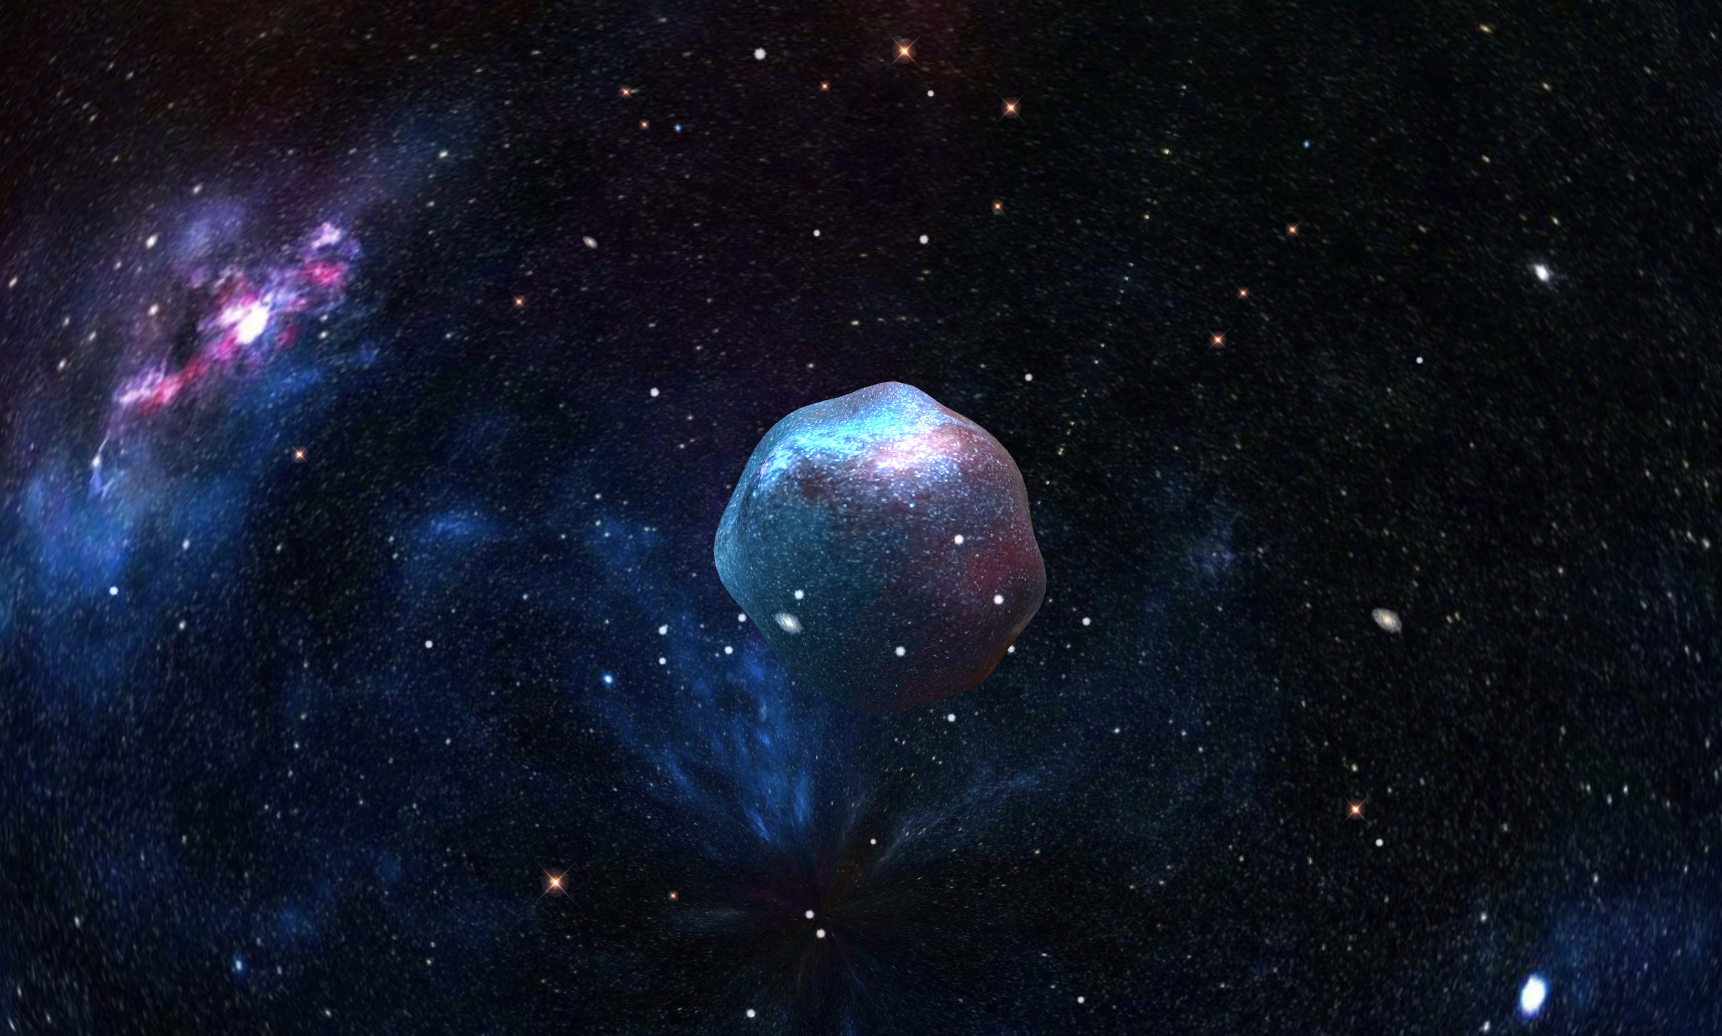
\includegraphics[width=9cm, keepaspectratio]{img/threejs.png}
  \caption{Escena creada con Three.js}\label{fig:three}
\end{figure}

Esta tecnología no solo sirve para la simple representación de las figuras en la escena si no que también es capaz de realizar ecuaciones matemáticas y crear matrices en la escena para dicha representación.

Gracias a Three.js se pueden construir las figuras de las escenas del editor, ya que A-Frame utiliza Three.js para dicha creación.

\section{HTML5} % título de sección (se muestra)
\label{sec:HTML5}
HTML~\cite{HTML} es uno de lo pilares fundamentales de este proyecto ya que es una de las tecnologías más usadas para la creación del mismo.

HTML es un lenguaje de marcado utilizado en el desarrollo del contenido web. Suele estar acompañado por otras tecnologías que la complementan, en cuanto a apariencia, CSS, no muy utilizada en este proyecto y en cuanto a funcionalidad, JavaScript, muy utilizada en este trabajo.

Una de las características de HTML es la utilización de marcas para etiquetar los distintos elementos del documento para luego mostrarlo en la web. Algunas de las etiquetas son: \begin{verbatim}<head>, <ul>, <p>, <span>.\end{verbatim} 

Estas etiquetas permiten al elemento tener una gran versatilidad, estructura lógica y facilidad a la hora de entenderlo. Dentro de estas podemos encontrar los atributos\footnote{\url{https://es.wikipedia.org/wiki/Atributo_HTM}} que son utilizados para controlar el comportamiento de dicha etiqueta.

Un ejemplo básico de un documento HTML puede ser el siguiente:

\begin{verbatim}
<!DOCTYPE html>
<html>
  <head>
    <meta charset="utf-8">
    <title>TFG Julián</title>
  </head>
  <body>
    <p>Hola mundo!</p>
  </body>
</html>
\end{verbatim}

Cuando hablamos de HTML es importante destacar el DOM, es la estructura de todos elementos del documento organizados en nodos, el conjunto de todos estos se denomina árbol de nodos. Gracias al DOM y al lenguaje JavaScript podremos acceder a los elementos para una libre utilización de ellos. Esta estructura es guardada en memoria por los navegadores y de este modo poder mostrar la página web al usuario.


\begin{figure}[H]
  \centering
  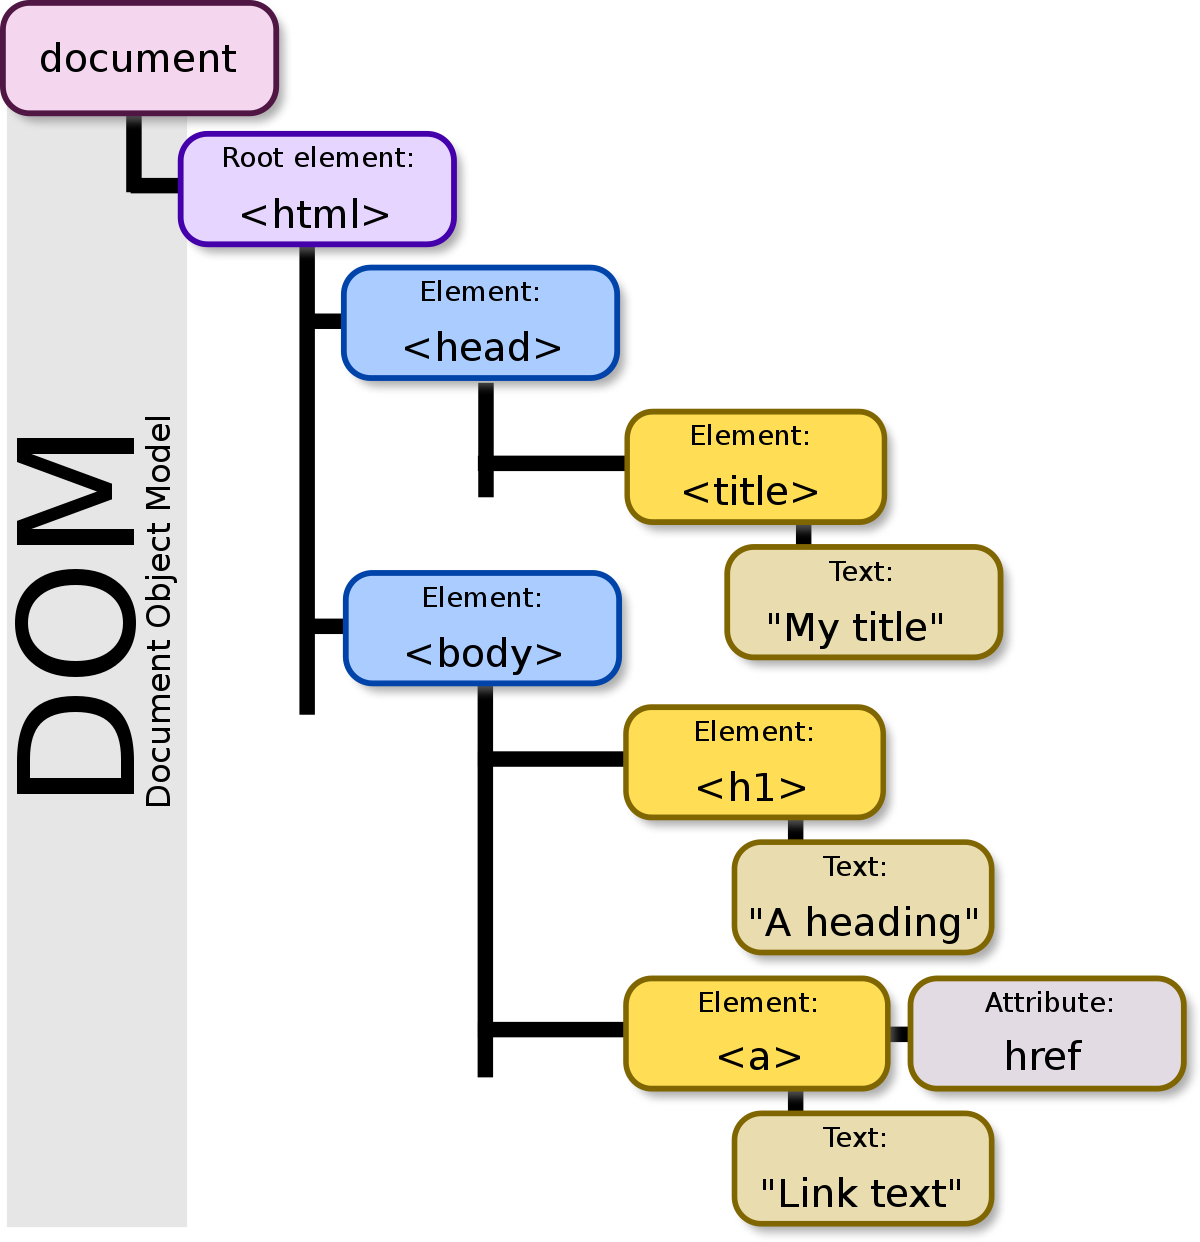
\includegraphics[width=7cm, keepaspectratio]{MemoriaTFG-JulianPerez/img/1200px-DOM-model.svg.png}
  \caption{Visualización gráfica del DOM}\label{html}
\end{figure}

Para terminar, destacar que ahora mismo HTML se encuentra en su versión HTML5, publicada en 2014, donde se añadieron varias nuevas funcionalidades como la inclusión de nuevas etiquetas o la compatibilidad con varias APIS con Canvas o WebGL.

En el editor de escenas, el framework, A-Frame, nos permite crear elementos mediante el lenguaje HTML.

\section{A-Frame} % título de sección (se muestra)
\label{sec:A-Frame}

Esta tecnología fue desarrollada por el equipo de mozilla VR durante 2015. El objetivo principal de estos era permitir crear dichas escenas directamente en HTML sin conocer WebGL. A parte de esta, también usa otras tecnologías anteriormente explicadas como son WebXR y JavaScript.

A-frame~\cite{a} es la tecnología más importante de este proyecto, ya que es la base fundamental de este. A-frame es un framework creado para la construcción de experiencias en realidad virtual, basado en HTML, por lo que como hemos dicho antes, es un lenguaje bastante sencillo e intuitivo. Una de las características claves de A-frame es el framework entidad-componente para Three.js.

Un ejemplo de creación de figuras en A-frame mediante HTML puede ser el siguiente:
\begin{verbatim}
<html>
  <head>
    <script src="https://aframe.io/releases/1.2.0/aframe.min.js">
    </script>
  </head>
  <body>
    <a-scene>
      <a-box position="-1 0.5 -3"></a-box>
      <a-sphere radius="1.25"></a-sphere>
      <a-cylinder color="#FFC65D"></a-cylinder>
      <a-planewidth="4" height="4"></a-plane>
      <a-sky color="#ECECEC"></a-sky>
    </a-scene>
  </body>
</html>
\end{verbatim}
El resultado en la página web de este código, es el siguiente:
\begin{figure}[H]
  \centering
  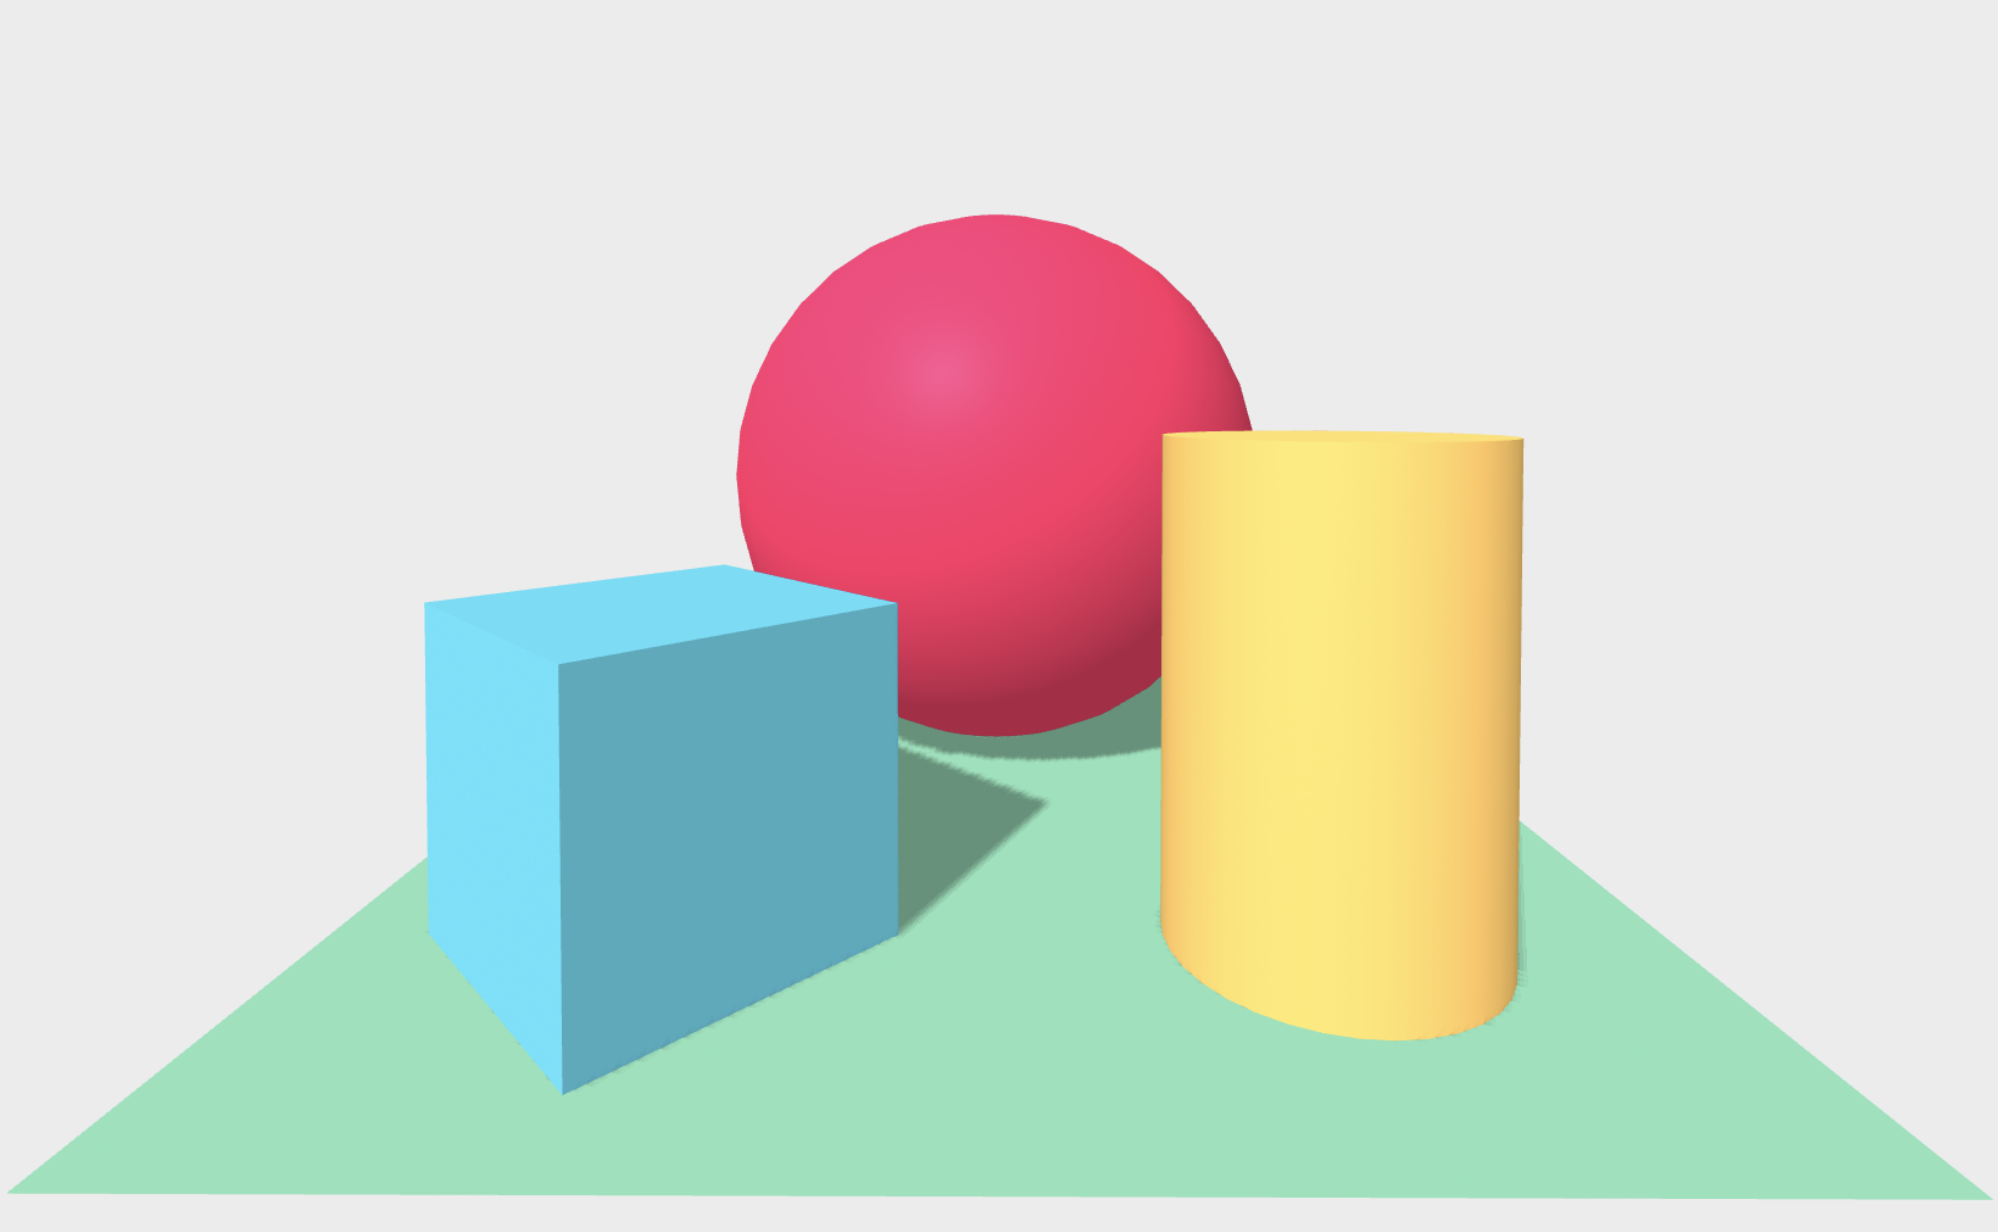
\includegraphics[width=12cm, keepaspectratio]{MemoriaTFG-JulianPerez/img/aframe.png}
  \caption{Escena básica A-Frame}\label{aframe}
\end{figure}
Explicando un poco más sobre el código del escenario de ejemplo, podemos destacar: 
\begin{itemize}
    \item La inclusión de las dependencias de A-Frame en el elemento Head, esto nos permite usar todos los elementos de esta tecnología.
    \item La creación de las diferentes figuras mediante sus respectivas etiquetas.
    \item Modificación de ciertos aspectos de las figuras mediante los atributos.
\end{itemize}
Profundizando un poco más sobre la relación entidad-componente, Una entidad es el objeto en sí creado mediante HTML y el componente es el comportamiento que le podemos asignar a dicha figura, estos se realiza en el JavaScript. 

Estos componentes siguen una estructura estandarizada, algunos elementos de dicha estructura son: schema el cual muestra las propiedades del componente e init, la parte del componente que se ejecuta al iniciar el componente. La manera correcta de incluir un componente a la escena es añadírselo al elemento como si de un atributo se tratara.

En mi aplicación, el uso de A-Frame ha sido fundamental, tanto para la creación de figuras como la creación de iluminación como la cámara del usuario y para el comportamiento de estos.

\section{GitHub} % título de sección (se muestra)
\label{sec:GitHub}
GitHub~\cite{GITHUB} es una plataforma de almacenamiento y administración  de software, Este sistema está basado en el control de versiones \footnote{\url{https://es.wikipedia.org/wiki/Control_de_versiones}} y en Git \footnote{\url{https://git-scm.com}}.

Gracias al control de versiones, el desarrollador puede administrar y llevar un registro de cualquier modificación sobre el proyecto. Este sistema permite al desarrollador trabajar de una forma segura mediante las ramas. Las ramas te permiten duplicar el código fuente, donde puede hacer cambios sin afectar al proyecto "principal". Puedes fusionar las distintas ramas si lo deseas.

En cuanto a Git, se trata de un sistema de control de versiones, es decir, te ayuda a controlar lo anterior explicado pero mediante el terminal del ordenador.

GitHub es una interfaz gráfica de Git el cual nos ofrece distintas funcionalidades como pueden ser, la creación de un usuario, la creación de distintos proyectos(repositorios) los cuales modificar desde la propia interfaz web, capacidad de trabajar en repositorios creados por otros desarrolladores mediante un fork\footnote{\url{https://es.wikipedia.org/wiki/Bifurcación_(desarrollo_de_software)}} o la modificación del mismo mediante un pull, creación de un foro en los que los desarrolladores pueden expresar dudas/problemas sobre el proyecto, etc.

Hoy en día según los desarrolladores  el 87\% de estos utilizan GitHub.

Para el desarrollo de mi aplicación GitHub ha sido la plataforma donde he alojado el código del mismo. También para el despliegue de esta, he utilizado GitHub pages, una funcionalidad de la página que te permite desplegar tus aplicaciones.

\section{PyCharm} % título de sección (se muestra)
\label{sec:GitHub}
Se trata de un entorno de desarrollo integrado (IDE) que se utiliza para la programación, es un software creado por la compañía JetBrains~\cite{jetbrains}.

Este software es multiplataforma adaptado para Windows, macOS y Linux. Ha sido utilizado para la creación de este proyecto y por eso es una parte fundamental de esto.

Tiene infinidad de ventajas entre las que están:

\begin{itemize}
    \item Asistencia y análisis de codificación, con ayuda a la finalización del código, sintaxis y resaltado de errores.
    \item Navegación entre proyectos y ficheros.
    \item Acceso a la ejecución del código en el navegador mediante accesos directos.
\end{itemize}

PyCharm proporciona una API para que los desarrolladores puedan crear distintos plugins y de este modo se pueda crear código de manera más fácil y eficiente.

Ha sido la herramienta utilizada para la creación del código del editor.

\section{LaTeX} % título de sección (se muestra)
\label{sec:Latex}
LaTeX está basado en Tex\footnote{\url{https://es.wikipedia.org/wiki/TeX}}, programa destinado a la creación de documentos que contienen textos y fórmulas matemáticas. Este programa no es un editor de textos, si no, un procesador de macros.

LaTeX es un conjunto de macros para Text, cuyo objetivo principal es la alta composición tipográfica. Está orientando a la producción y creación de documentos científicos y se ha estandarizado para la creación de los mismos.

Esta tecnología nos presenta diversas ventajas entre las que se encuentran la facilidad de gestionar las referencias, bibliografías, etc, es un sistema multiplataforma, puedes componer fórmulas con calidad de imprenta o la capacidad de exportar el documento a PDF. La creación de dichos documentos puede ser al principio, un poco complicado si no se conoce la herramienta.

Se trata de un software libre bajo la licencia LPPL\footnote{\url{https://es.wikipedia.org/wiki/LaTeX_Project_Public_License}} 

Este sistema ha sido fundamental a la hora de crear este proyecto ya que esta memoria esta creada utilizando LaTeX.

\section{glTF} % título de sección (se muestra)
\label{sec:Gltfs}
Este formato de archivo tiene como objetivo principal escenas y modelos en 3D y esta basado en el formato de texto sencillo para el intercambio de datos, JSON. Popularmente se le describe como como el JPEG en 3D.

Este formato está creado para una eficiente distribución de objetos y escenas en 3D, disminuyendo el tiempo de procesamiento en ejecución. Este formato se puede usar en aplicaciones que usan la tecnología anteriormente explicada, WebGL.

Es importante explicar este formato, ya que la aplicación que he creado te permite el manejo y  modificación de este formato en la aplicación.

\section{Trabajos relacionados} % título de sección (se muestra)
\label{sec:Otros}
Cabe destacar algunos editores que han servido como inspiración para la creación de mi editor como son Blender, centrado en aspectos como la renderización o la creación de gráficos en 3D o Unity centrado en creación del motor gráfico en videojuegos. 

%%%%%%%%%%%%%%%%%%%%%%%%%%%%%%%%%%%%%%%%%%%%%%%%%%%%%%%%%%%%%%%%%%%%%%%%%%%%%%%%
%%%%%%%%%%%%%%%%%%%%%%%%%%%%%%%%%%%%%%%%%%%%%%%%%%%%%%%%%%%%%%%%%%%%%%%%%%%%%%%%
% ESTADO DEL ARTE %
%%%%%%%%%%%%%%%%%%%%%%%%%%%%%%%%%%%%%%%%%%%%%%%%%%%%%%%%%%%%%%%%%%%%%%%%%%%%%%%%

\cleardoublepage
\chapter{Desarrollo del proyecto}
\label{chap:Desarrollo del proyecto}
Centrándonos en el desarrollo del proyecto debemos comenzar explicando la metodología SCRUM~\cite{proyectos} ya que hemos seguido una metodología muy similar para la creación de este proyecto.

Está metodología, oficialmente surgió en 1995 presentado por Ken Schwaber y Jeff Sutherland mediante "SCRUM Development Process". Aunque esta fuera la fecha oficial, este modelo ya se había dejado ver en los años 80.

SCRUM es un metodología que está centrada en el desarrollo ágil\footnote{\url{https://es.ryte.com/wiki/Desarrollo_Ágil_de_Software}}  de software, aunque he realizado el proyecto de manera individual esta metodología se suele aplicar de manera colectiva con la participación en equipo con el objetivo de obtener el mejor resultado posible.

En Scrum se pueden diferenciar distintos roles, Scrum Master, Product owner y el equipo. El rol de SCRUM Master en este caso esta representado por el tutor del proyecto cuya función es facilitar y ayudar a gestionar el trabajo. En este caso el product owner no tiene un papel importante y respecto al equipo está representado por mí, el alumno que realiza este proyecto, y su función es el desarrollo y la entrega de las distintas tareas organizadas en cada sprint.

Durante los sprints el equipo, en este caso yo, me centraré en la realización de las tareas marcadas. Estos sprint se inician con un reunión Scrum Master - equipo en la cual se fijaba unos objetivos y se marcaban los pasos a seguir para la consecución de dichos objetivos. Tras un tiempo trabajando en el sprint se emplaza otra nueva reunión en la cual se comparte la tarea terminada y los problemas que han ido surgiendo durante esta. En esta misma reunión el equipo prepara un versión funcional de la aplicación o tarea y se marcan los siguientes pasos a seguir. 

Se puede ver más en detalle el proceso en la siguiente imagen:
\begin{figure}[H]
  \centering
  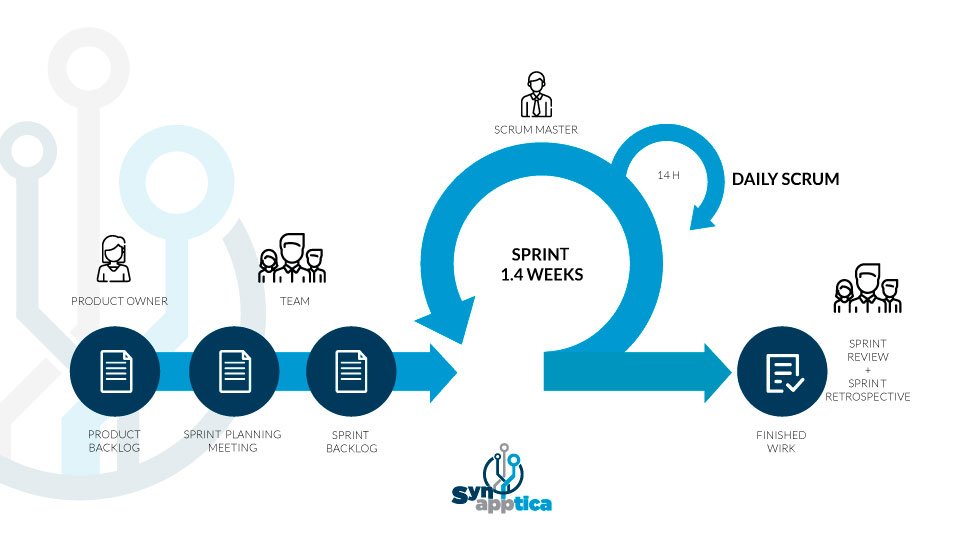
\includegraphics[width=12cm, keepaspectratio]{MemoriaTFG-JulianPerez/img/Scrum.jpg}
  \caption{Estructura metodología Scrum}\label{scrum}
\end{figure}

\section{Sprint 0} % título de sección (se muestra)
\label{sec:sprint0}
En este primer sprint el Scrum Master comenzó a introducir las principales tecnologías que iban a ser usadas en el proyecto, A-frame, JavaScript y HTML. Por lo que en este sprint me dedique a realizar una actividad que asentará la unión entre ambas tecnologías.

\subsection{Objetivo}
El objetivo principal de este Sprint es empezar a usar A-Frame para poder así introducirme en la tecnología y aprender como utilizarla. la creación de distintas entidades, eventos, componentes y físicas son los principales objetivos. En este sprint tenemos que tener en cuenta que una de las principales tecnologías utilizadas, JavaScript, era nueva para mí, por lo que también tuve que aprender sobre esta. Para consolidar todo lo anterior la tarea a realizar fue la creación de un mini juego en el que crear un componente y que este, reaccionara a un evento.

\subsection{Desarrollo}
Todo comienza haciéndose una idea de que va a tratar el mini juego, que componente vamos a crear y que comportamiento le vamos a dar.

La base fundamental del mini juego será un recorrido en el cual debes adivinar una de las tres puertas que hay en las diferentes secciones para así, poder avanzar y llegar al objetivo final del juego.

Para el comportamiento de choque contra la pared, que tendrás que realizar para pasar a la siguiente sección utilizaremos el componente Kinema.js que nos proporciona las físicas necesarias para esto. 

El recorrido creado es muy sencillo y presentas las siguientes fases:

\begin{itemize}
    \item Cuando entramos en el juego nos encontramos con la primera sección de tres puertas a adivinar, además, si giramos la cámara nos encontramos con las instrucciones del juego.
    \begin{figure}[H]
  \centering
  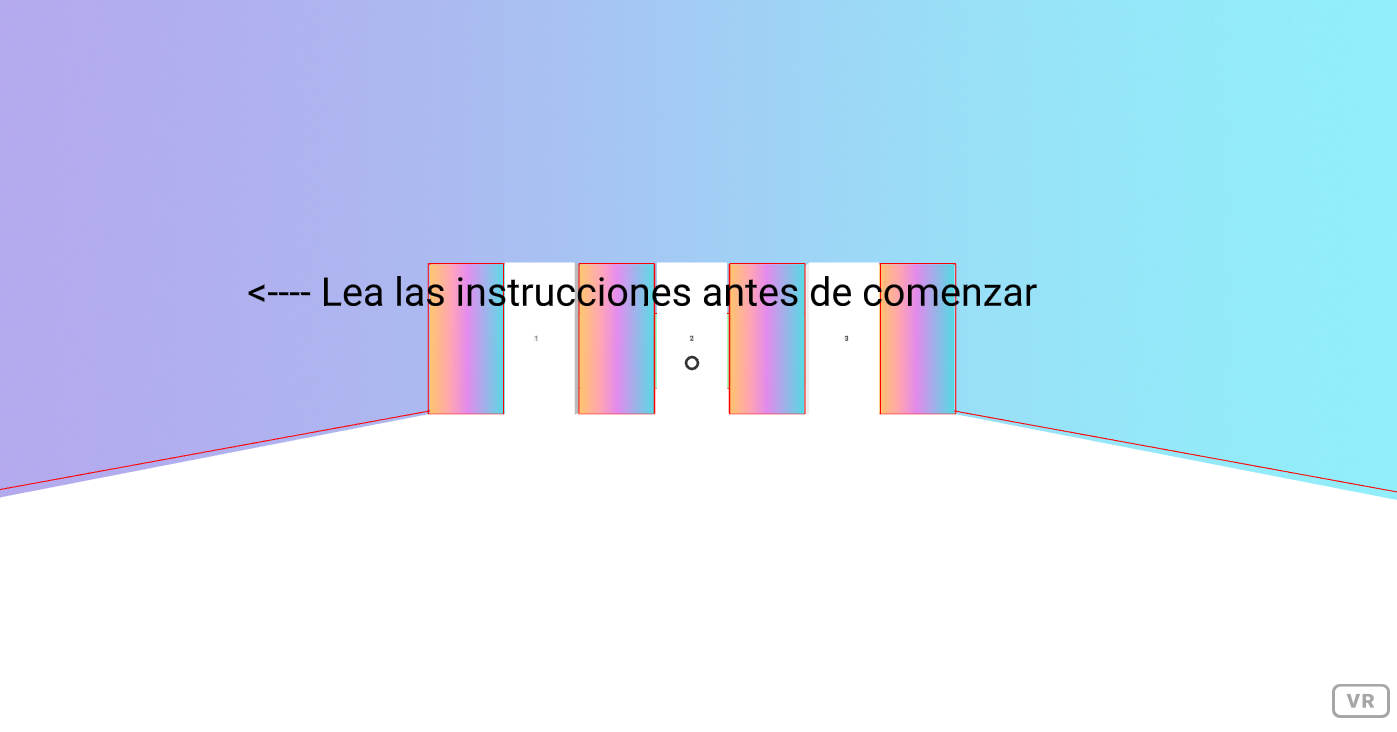
\includegraphics[width=12cm, keepaspectratio]{MemoriaTFG-JulianPerez/img/mini.png}
  \caption{Incio mini juego}\label{scrum}
\end{figure}
    \item Tras esto nos encontramos con tres secciones en las cuales debemos adivinar la puerta para poder avanzar a la siguiente. La manera que tenemos de pasar a la siguiente sección es empujando la puerta, si es la puerta correcta, dicha puerta caerá y podrás pasar a la siguiente.
     \begin{figure}[H]
  \centering
  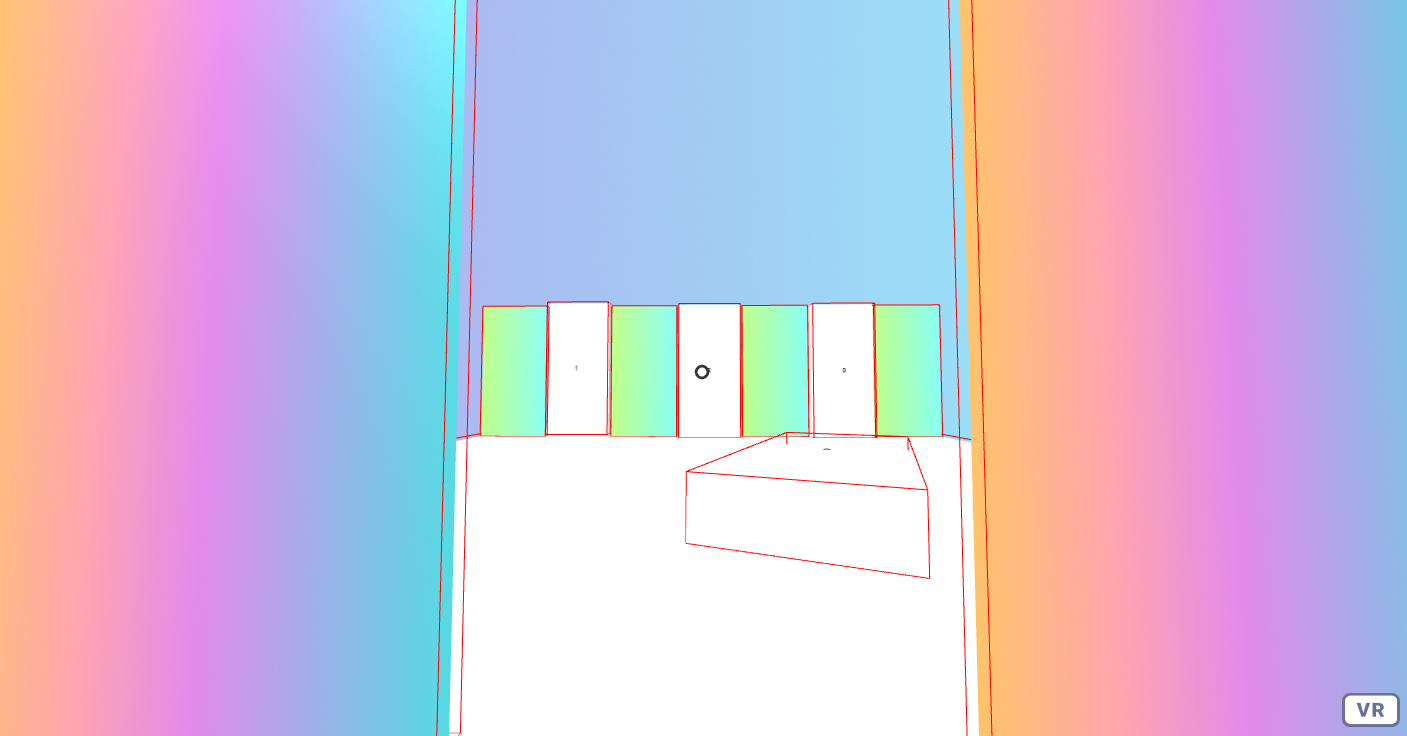
\includegraphics[width=12cm, keepaspectratio]{MemoriaTFG-JulianPerez/img/suelo.png}
  \caption{Situación siguiente sección}\label{scrum}
\end{figure}
    \item Por último tras adivinar todas la puertas, nos encontramos con el objetivo principal del juego, pulsar el botón de la victoria, al cual solo se puede llegar atravesando las puertas. Tras pulsar este botón, el texto que se encuentra en la parte superior te indicará que has ganado.
         \begin{figure}[H]
  \centering
  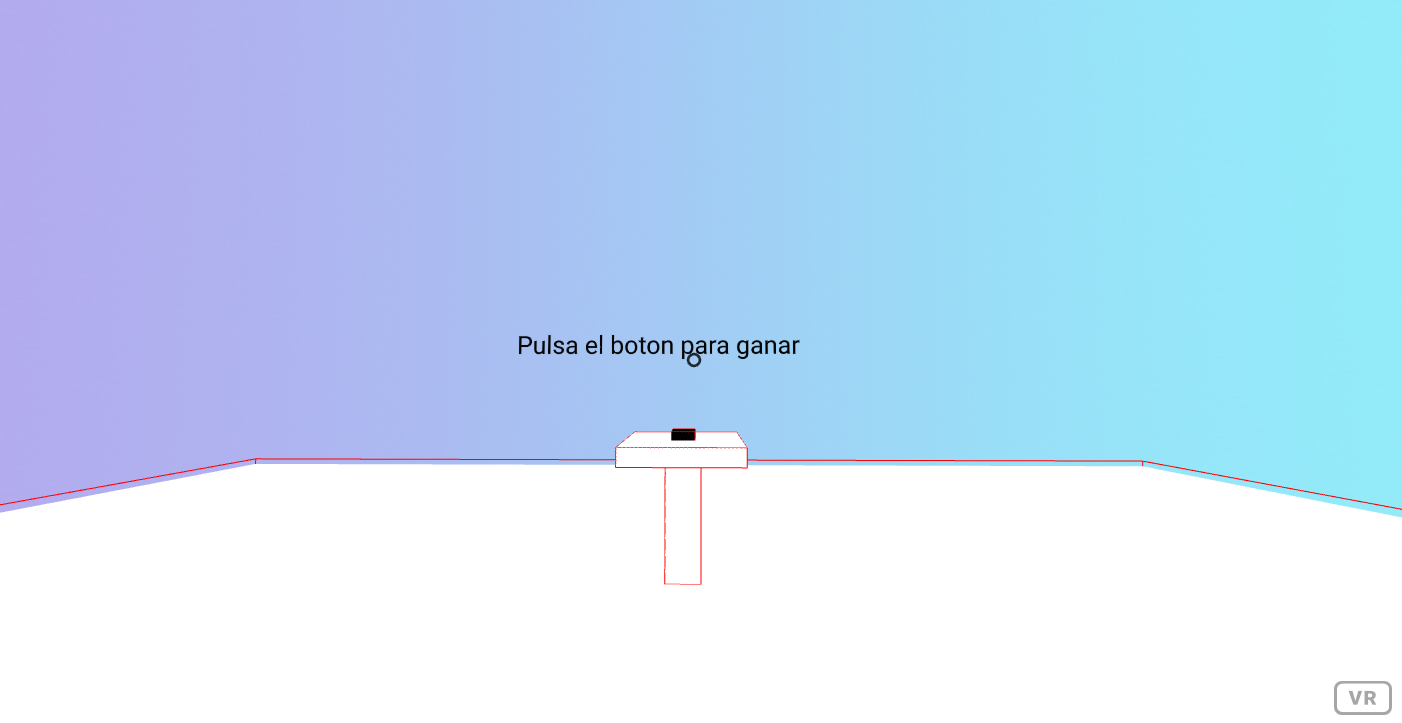
\includegraphics[width=12cm, keepaspectratio]{MemoriaTFG-JulianPerez/img/last.png}
  \caption{Parte final mini juego}\label{scrum}
\end{figure}

\end{itemize}

En cuanto al código creado para este mini juego , cabe destacar lo siguiente:
\begin{verbatim}
<script src="//cdn.rawgit.com/donmccurdy/aframe-physics-system/
v4.0.1/dist/aframe-physics-system.min.js"></script>
<script src="//cdn.rawgit.com/donmccurdy/aframe-extras/
v5.0.0/dist/aframe-extras.min.js"></script>
<script src="components/kinema.js"></script>
\end{verbatim}  
Estas líneas de código localizadas en el elemento \begin{verbatim}
<head>
\end{verbatim} son componentes que nos permiten utilizar distintas funcionalidades que aplicaremos en nuestro mini juego, como puede ser la creación de distintas entidades o la utilización de físicas.

Otra línea de código interesante es:
\begin{verbatim}
<a-box dynamic-body><a-text></a-text></a-box>
<a-box static-body><a-text></a-text></a-box>
\end{verbatim} 

Esta parte de código  trata de una parte de la creación de las puertas que tienes que elegir, estas, utilizan un componente que proporciona el comportamiento de una entidad fija o movible.\begin{verbatim}dynamic-body/static-body \end{verbatim}

Por ultimo cabe destacar un sencillo componente creado por mí, cuya función es el cambio del texto al pulsar en una entidad.Este texto muestra al usuario que ha conseguido el objetivo del mini juego.  Este era realmente el objetivo del sprint la creación de una entidad que reaccionara a un evento.

La estructura de un componente es la siguiente:
\begin{verbatim}
AFRAME.registerComponent('nowinnertowinner', {
schema: {
},
init: function () {

},
\end{verbatim} 

         \begin{figure}[H]
  \centering
  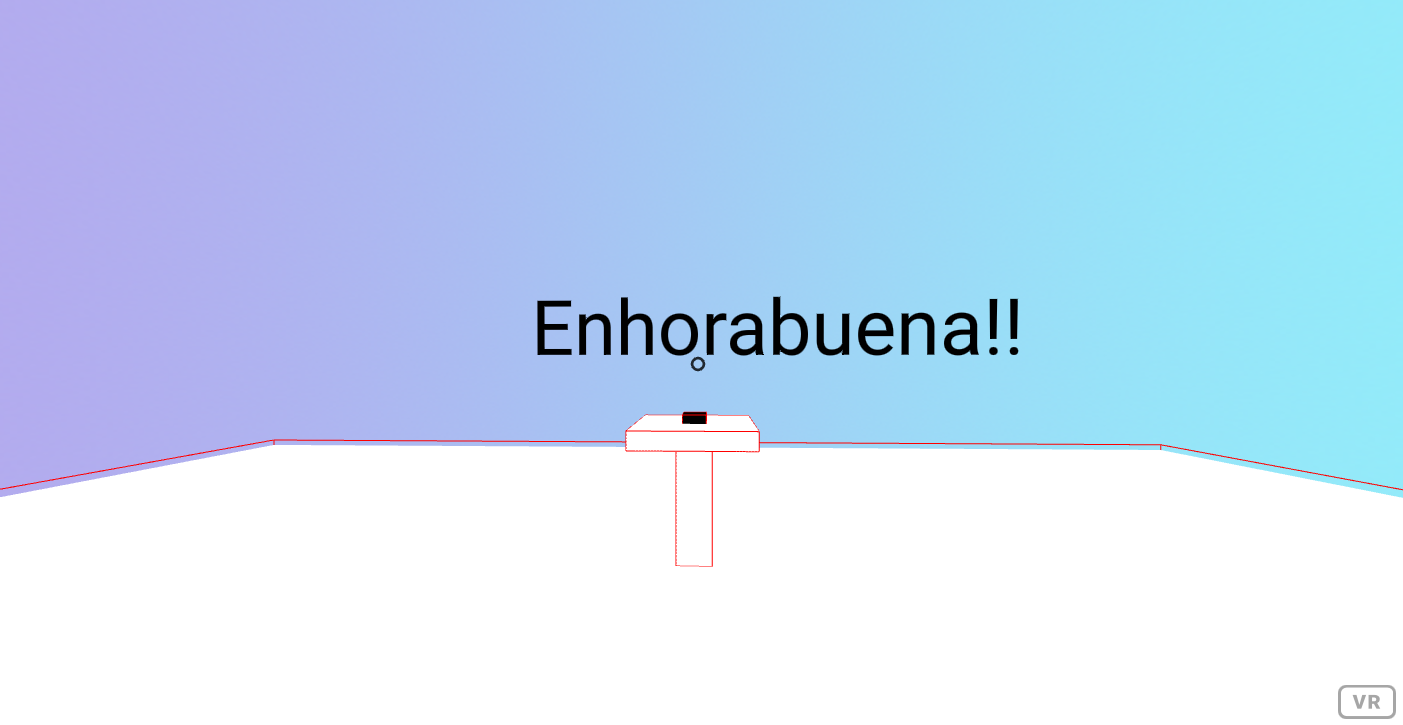
\includegraphics[width=12cm, keepaspectratio]{MemoriaTFG-JulianPerez/img/lastwin.png}
  \caption{Mini juego completado}\label{scrum}
\end{figure}

\subsection{Resultado}
En este primer sprint aprendí las posibilidades que nos puede dar a-frame y a hacerme una idea de como plantear el resto del proyecto, de manera paralela fui aprendiendo a utilizar JavaScript ya que era una tecnología muy poco antes usada. Este mini juego se encuentra en el repositorio del proyecto y esta accesible a cualquier persona tanto a la interfaz del juego\footnote{\url{https://julianperezm.github.io/A-frame/FirstExercise/FirstExercise.html}}  como al código\footnote{\url{https://github.com/julianperezm/A-frame/tree/master/FirstExercise}} . Tras esto, se mantuvo la correspondiente reunión con el SCRUM Master en la cual se pone en común lo aprendido y se plantea el siguiente sprint.

\section{Sprint 1}
A partir de este sprint se empezará a construir nuestra aplicación final por lo que podemos decir que este sprint es la base de nuestro proyecto. 
\subsection{Objetivo}
El objetivo de este sprint es la creación de un menú con las cuatro formas básicas de A-Frame (plano, cubo, cilindro y esfera). las cuales las podremos seleccionar y aparecerán en un lugar determinado de la escena. Para la creación de estas acciones utilizaremos tanto elementos HTML como componentes creados en JavaScript.

\subsection{Desarrollo}
Algunos sprints los separaremos en tareas para así organizar mejor este y poder así trabajar lo más eficiente posible.

\textbf{Tarea 1}

En esta primera tarea crearemos un menú con cuatros figuras básicas.El modo de interactuar con dichas figuras, es  mediante el cursor clicando encima de ellas. De este modo las figuras apareceran en el escenario.
El resultado de esta tarea se puede visualizar en la figura 3.6
\begin{figure}[H]
  \centering
  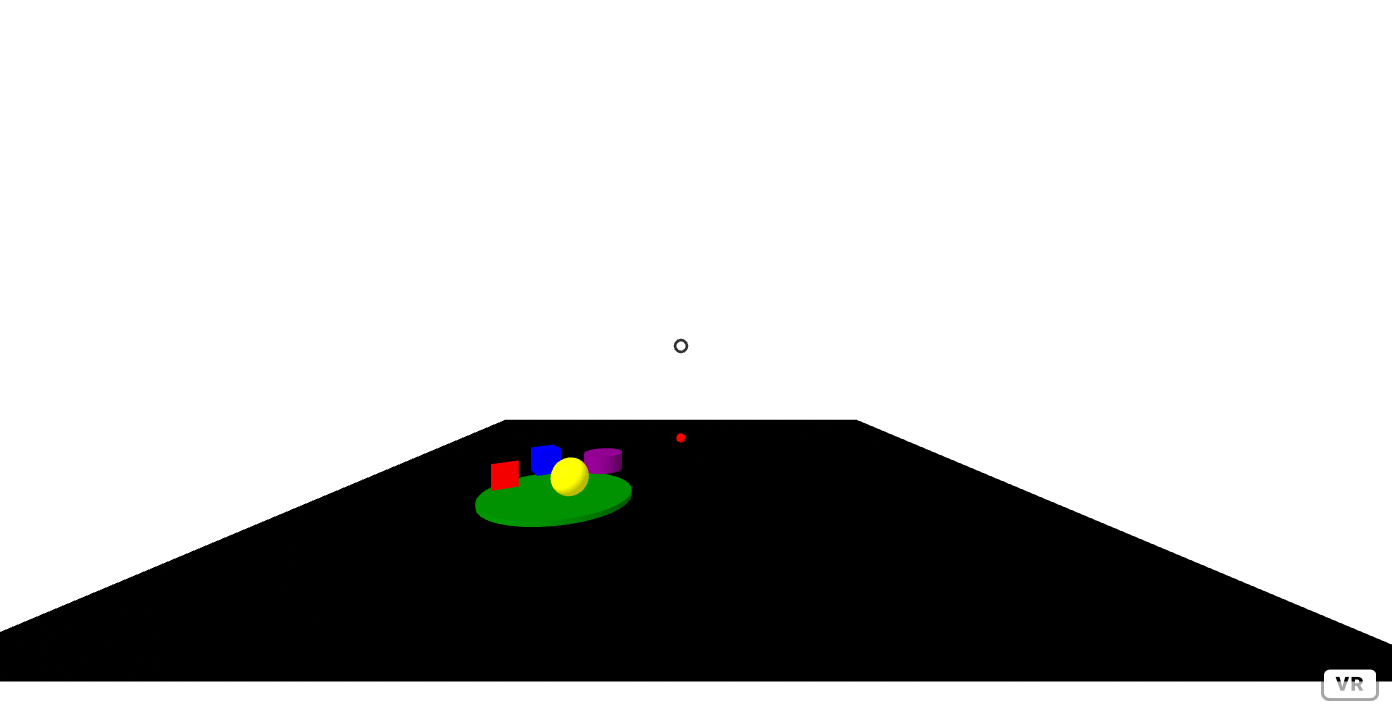
\includegraphics[width=12cm, keepaspectratio]{MemoriaTFG-JulianPerez/img/1.png}
  \caption{Inicio primer ejercicio}\label{scrum}
\end{figure}

\textbf{Tarea 2}

En nuestro camino hacia el objetivo añadiremos movimiento al menú para hacerlo más accesible al usuario, utilizaremos el atributo  de animación para la creación de la tarea.
\begin{verbatim}
 baseMenu.setAttribute('animation', 'property:rotation;to:0 360 0;
 loop:true;dur:10000')   
\end{verbatim}

\textbf{Tarea 3}

En esta tarea seguimos con la funcionalidad de crear una interfaz más amigable y pulsar una figura con el cursor de A-Frame no lo era. Por lo que creamos una interacción con la figura clicando directamente en ellas. A su vez también cambiamos el aspecto del escenario para que fuera mas vistoso al usuario. Como se puede ver en la figura 3.7.
         \begin{figure}[H]
  \centering
  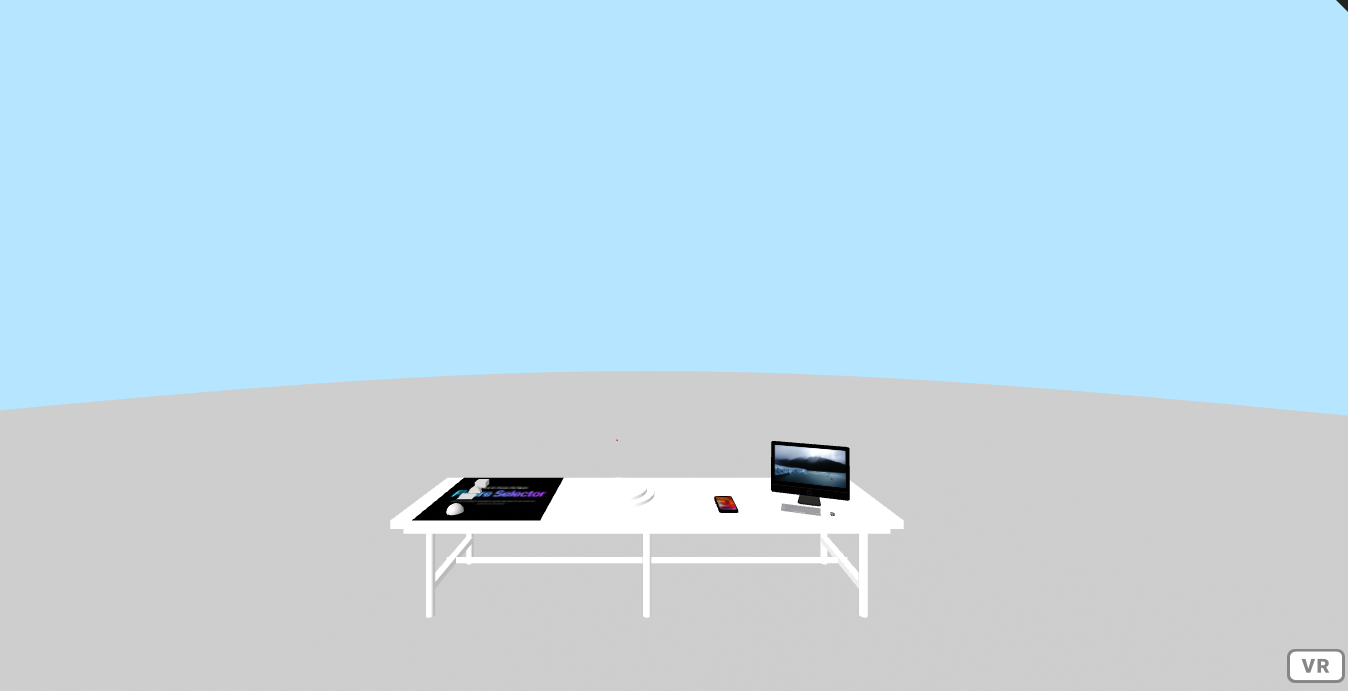
\includegraphics[width=12cm, keepaspectratio]{MemoriaTFG-JulianPerez/img/2.png}
  \caption{Escena inicial con mejora en la interfaz}\label{scrum}
\end{figure}

\textbf{Tarea 4}

Para seguir adelante con la creación del editor, en esta tarea nos centraremos en la funcionalidad, la cual permitirá que las figuras puedan ser arrastradas a cualquier lugar de la escena y que cada una tenga una mini previsualización de distintos colores encima de ella.          
\begin{figure}[H]
  \centering
  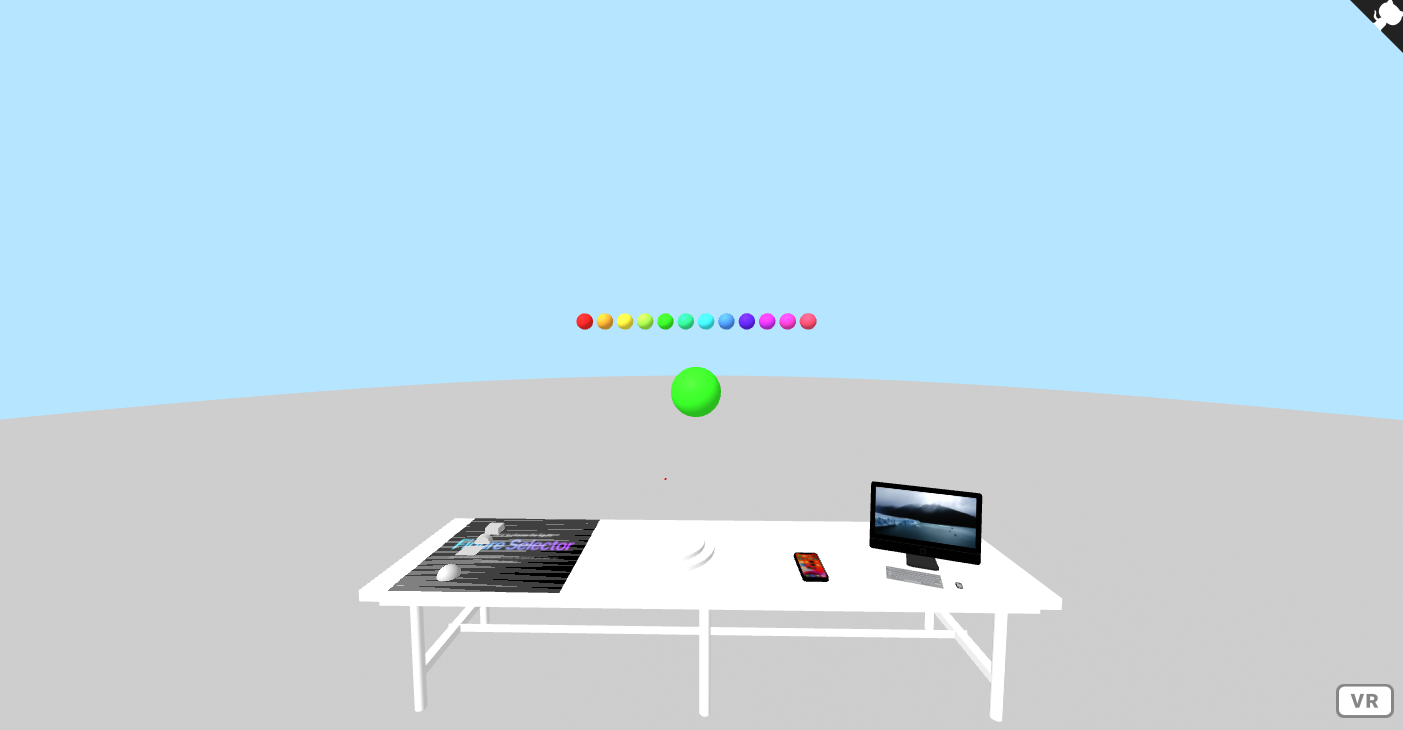
\includegraphics[width=12cm, keepaspectratio]{MemoriaTFG-JulianPerez/img/3.png}
  \caption{Figura creada en la escena}\label{scrum}
\end{figure}

\textbf{Tarea 5}

Por último en esta tarea se empieza a jugar con la creación de modelos en 3D con el formato glTF explicado anteriormente. Insertamos en la escena un dispositivo móvil y un ordenador a modo de decoración, como se observa en la figura 3.9.
\begin{figure}[H]
  \centering
  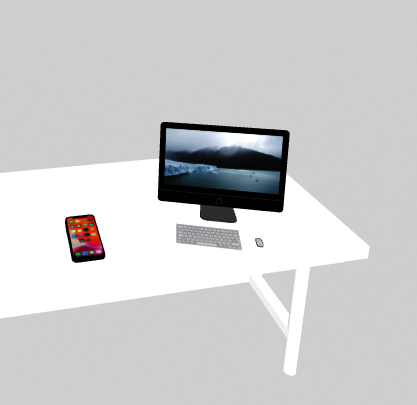
\includegraphics[width=12cm, keepaspectratio]{MemoriaTFG-JulianPerez/img/4.png}
  \caption{Modelos 3D en la escena}\label{scrum}
\end{figure}

\subsection{Resultado}
En este sprint se dio el primer paso de lo que será nuestro editor, se comienza con la creación de algunas de las funcionalidades finales de la aplicación. Toda esta implementación se encuentra en el repositorio del proyecto en GitHub,tanto al código \footnote{\url{https://github.com/julianperezm/A-frame/tree/master/ThirdExercise}} HTML o JavaScript como a la escena en el navegador\footnote{\url{https://julianperezm.github.io/A-frame/ThirdExercise/ThirdExercise.html}}

\section{Sprint 2}
En este sprint tras haber empezado este proyecto, nos centraremos en distintas funcionalidades y la mejora de la interfaz de la aplicación.

\subsection{Objetivo}
Nos centraremos en tres objetivos principales, 

\begin{itemize}
    \item La modificación de una propiedad concreta de las figuras, el tamaño.
    \item Una de las funcionalidades principales de la aplicación, la creación de un modo grupo de figuras.
    \item La mejora de la interfaz de la aplicación para que sea mas usable en 3D.
\end{itemize}

\subsection{Desarrollo}
Como en los casos anteriores separaremos el desarrollo del sprint en diferentes tareas.

\textbf{Tarea 1}

En esta tarea me centraré en la creación de la funcionalidad que llamaré, modo grupo. Esta funcionalidad consiste en la unión de diferentes figuras que serán manejadas por otra que llamaremos, manejador. 

Esta funcionalidad es útil por si queremos crear una figura que se base en la unión de varias. Él método por el que realizaremos esta funcionalidad es mediante la creación de distintos componentes. La manera de acceder a ella es pulsando la tecla q. 

El resultado de esta tarea se puede observar en un panel creado en el escenario, cuando el modo grupo este activado se mostrará como se puede observar en la figura 3.11, del mismo modo cuando esté activado figura 3.10.

\begin{figure}[H]
  \centering
  \begin{minipage}[b]{0.4\textwidth}
 
\includegraphics[width=7cm]{MemoriaTFG-JulianPerez/img/single.png}
  \caption{Modo grupo desactivado}\label{single}
  \end{minipage}
  \hfill
  \begin{minipage}[b]{0.4\textwidth}
  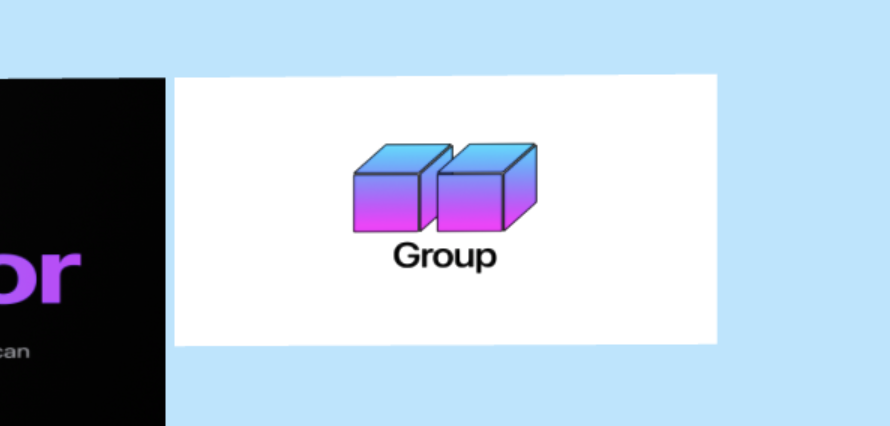
\includegraphics[width=7cm]{MemoriaTFG-JulianPerez/img/group.png}
  \caption{Modo grupo activado}\label{scrum}
  \end{minipage}
\end{figure}

\textbf{Tarea 2}

Tras la creación de la funcionalidad, me centraré en la modificación de una de las propiedades de la figura. La modificación se centra en el tamaño, recordemos que anteriormente añadimos el poder cambiar el color de la figura.

Esto lo realizaré de una manera similar, crear distintos componentes que permitan modificar la escala de la figura, con una particularidad, podremos modificar la escala en los distintos ejes para así poder tener más posibilidades a la hora de crear diferentes figuras. 

Esta tareas se puede visualizar en la escena mediante diferentes botones que se pueden ver en la figura 3.12 además de esto, podrás ver las medidas de la figura creada.

\begin{figure}[H]
  \centering
  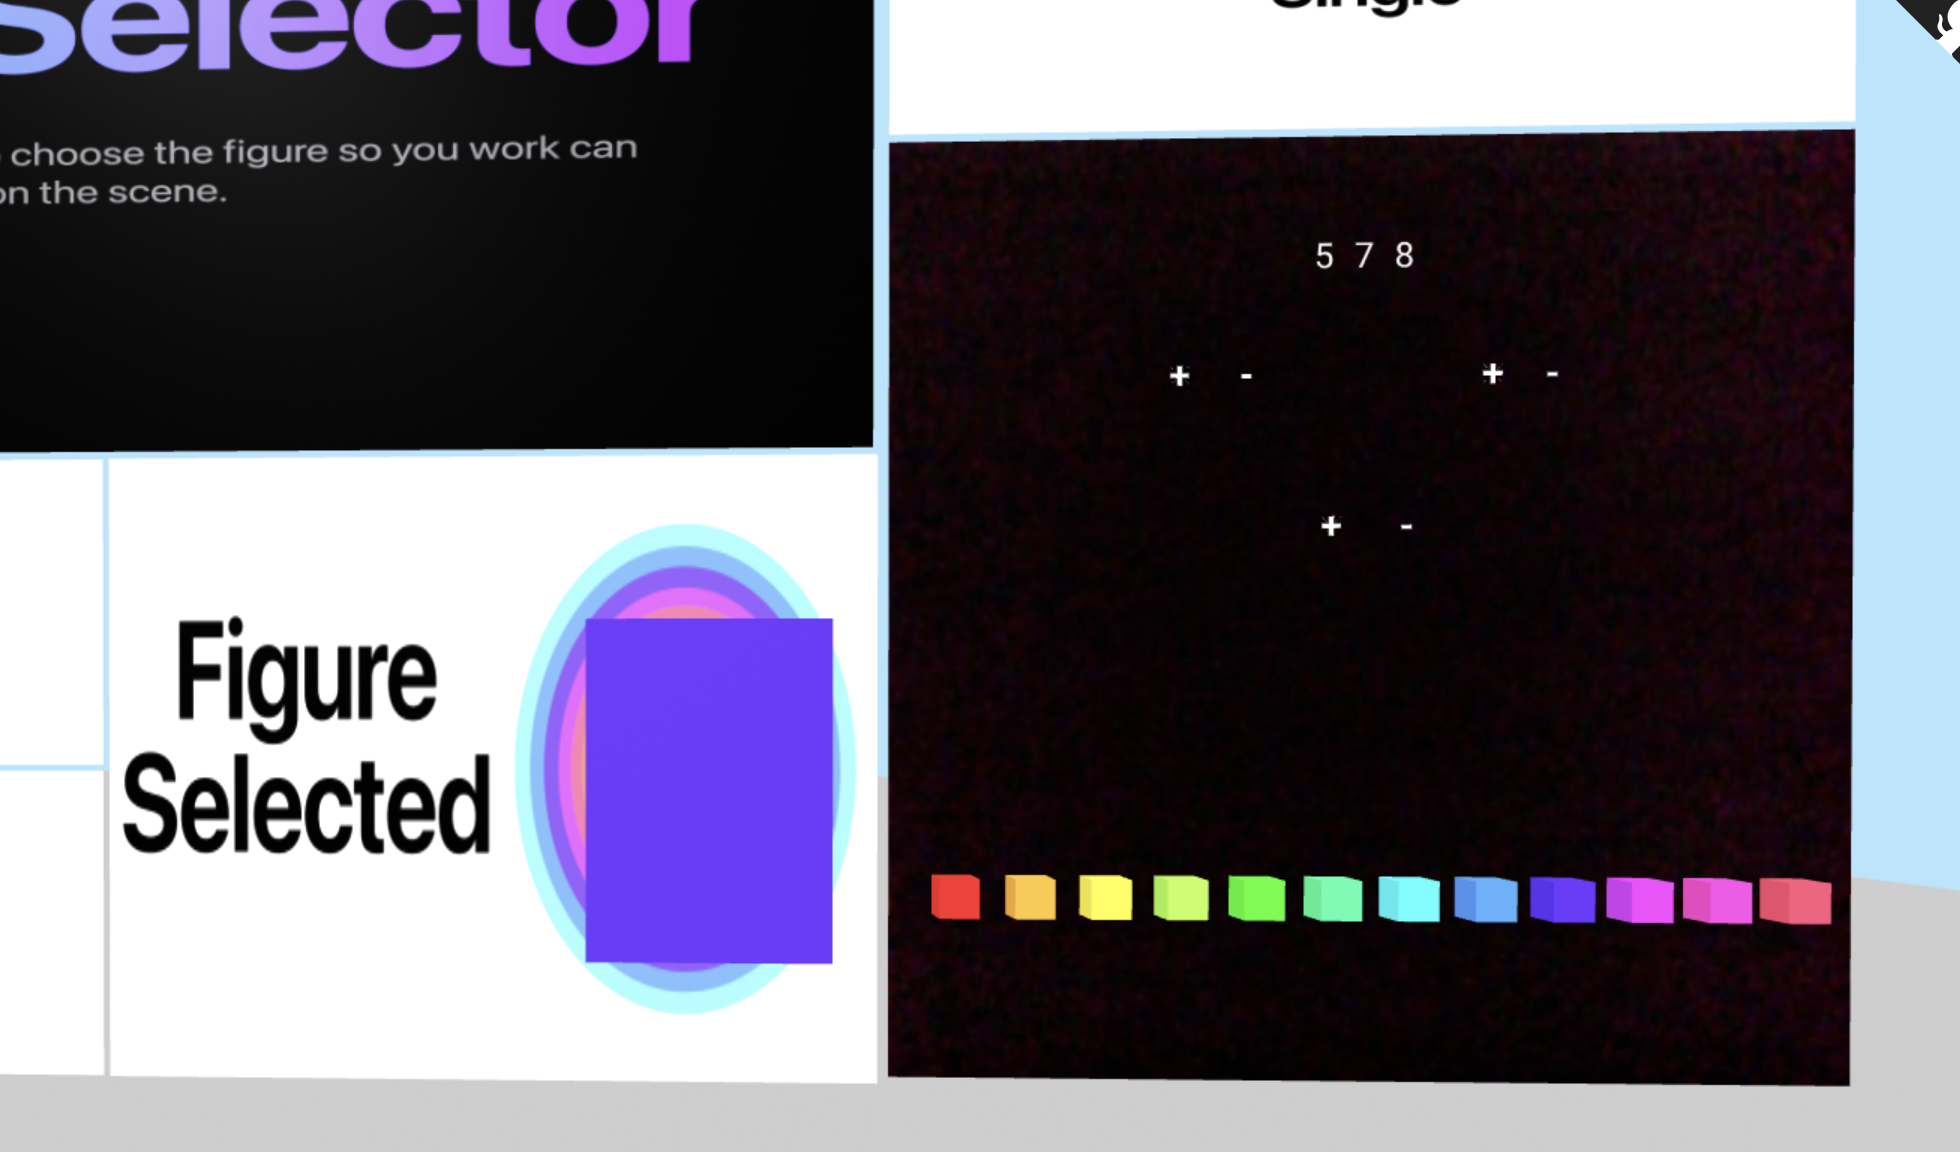
\includegraphics[width=12cm, keepaspectratio]{MemoriaTFG-JulianPerez/img/tam.png}
  \caption{Menú modificación figura}\label{scrum}
\end{figure}

\textbf{Tarea 3}

En esta tarea nos centraremos en la mejora de la interfaz de la aplicación para que sea más usable y mas vistosa para el usuario. 

Los paneles de información de la aplicación en lugar de ser planos se les dará un poco de profundidad, el menú de selección de figuras, pasará a ser en 3D para que sea mas intuitivo, para realizar este cambio se modifico el atributo de tamaño de todos los elementos del menú añadiéndoles profundidad.

El resultado se puede observar en la figura 3.13

\begin{figure}[H]
  \centering
  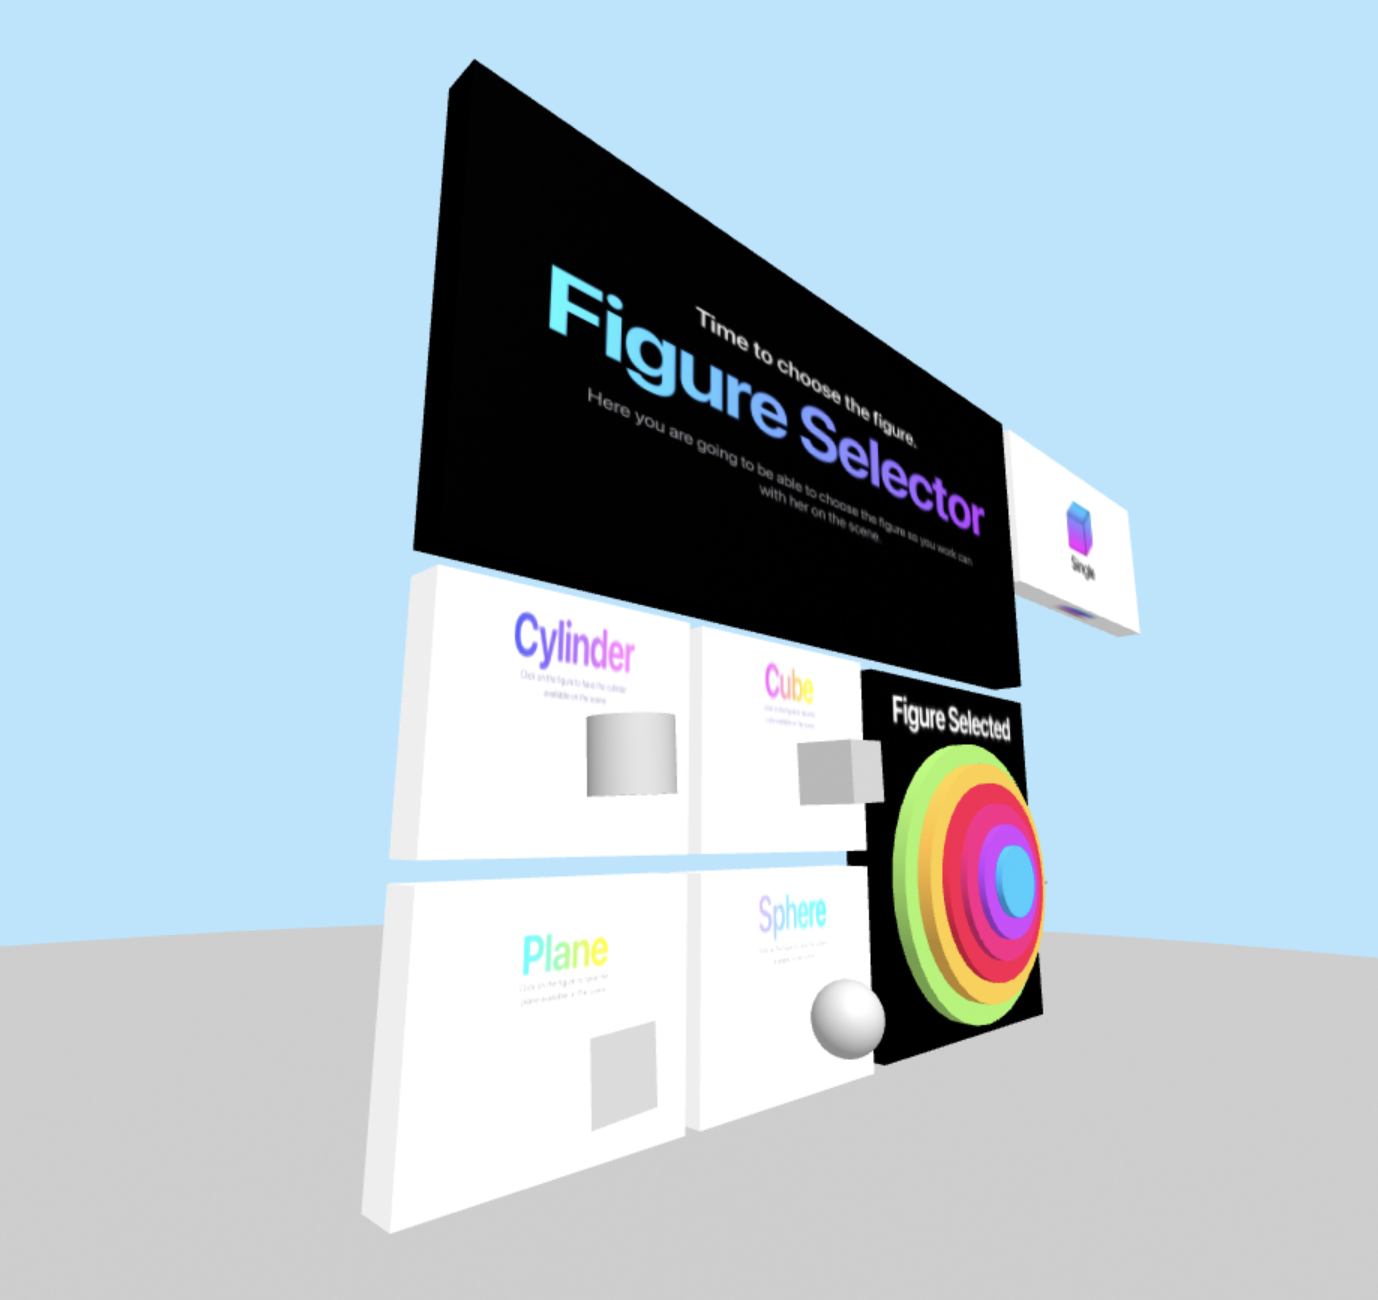
\includegraphics[width=12cm, keepaspectratio]{MemoriaTFG-JulianPerez/img/prof.png}
  \caption{Nueva interfaz de la aplicación}\label{scrum}
\end{figure}

\subsection{Resultados}

En este sprint hemos conseguido mejorar considerablemente nuestro editor, ya que hemos añadido una nueva funcionalidad, hemos añadido un método más de modificación de la figura y hemos mejorado el escenario para un uso mas fácil de este. Este sprint está disponible en el repositorio del proyecto en GitHub, tanto el código\footnote{\url{https://github.com/julianperezm/A-frame/tree/master/FifthExerciseV1}} como el escenario \footnote{\url{https://julianperezm.github.io/A-frame/FifthExerciseV1/FifthExercise.html}}.


\section{Sprint 3}

Tras el sprint anterior en este seguiremos mejorando la interfaz de usuario de la aplicación además de añadirle nuevas funcionalidades como la creación de nuevas figuras y la modificación de nuevos atributos de estas.

\subsection{Objetivo}
Para este sprint tenemos varios objetivos en los que centrarnos:
\begin{itemize}
    \item Mejora de la interfaz, me centraré en distintos puntos como son las dimensiones del escenario y la visibilidad de distintos objetos.
    \item Añadiré la funcionalidad de poder añadir nuevas figuras con el formato glTF.
    \item Compatibilizar la aplicación con las gafas de realidad aumentada.
\end{itemize}

\subsection{Desarrollo}
Las tareas para este sprint son las siguientes:

\textbf{Tarea 1}

En esta tarea me centraré en la mejora de la interfaz de usuario. Rediseñaremos el escenario, Respecto del tamaño, lo haremos más pequeño, ya que anteriormente las figuras no tenían un tamaño acorde con el escenario.

\begin{figure}[H]
  \centering
  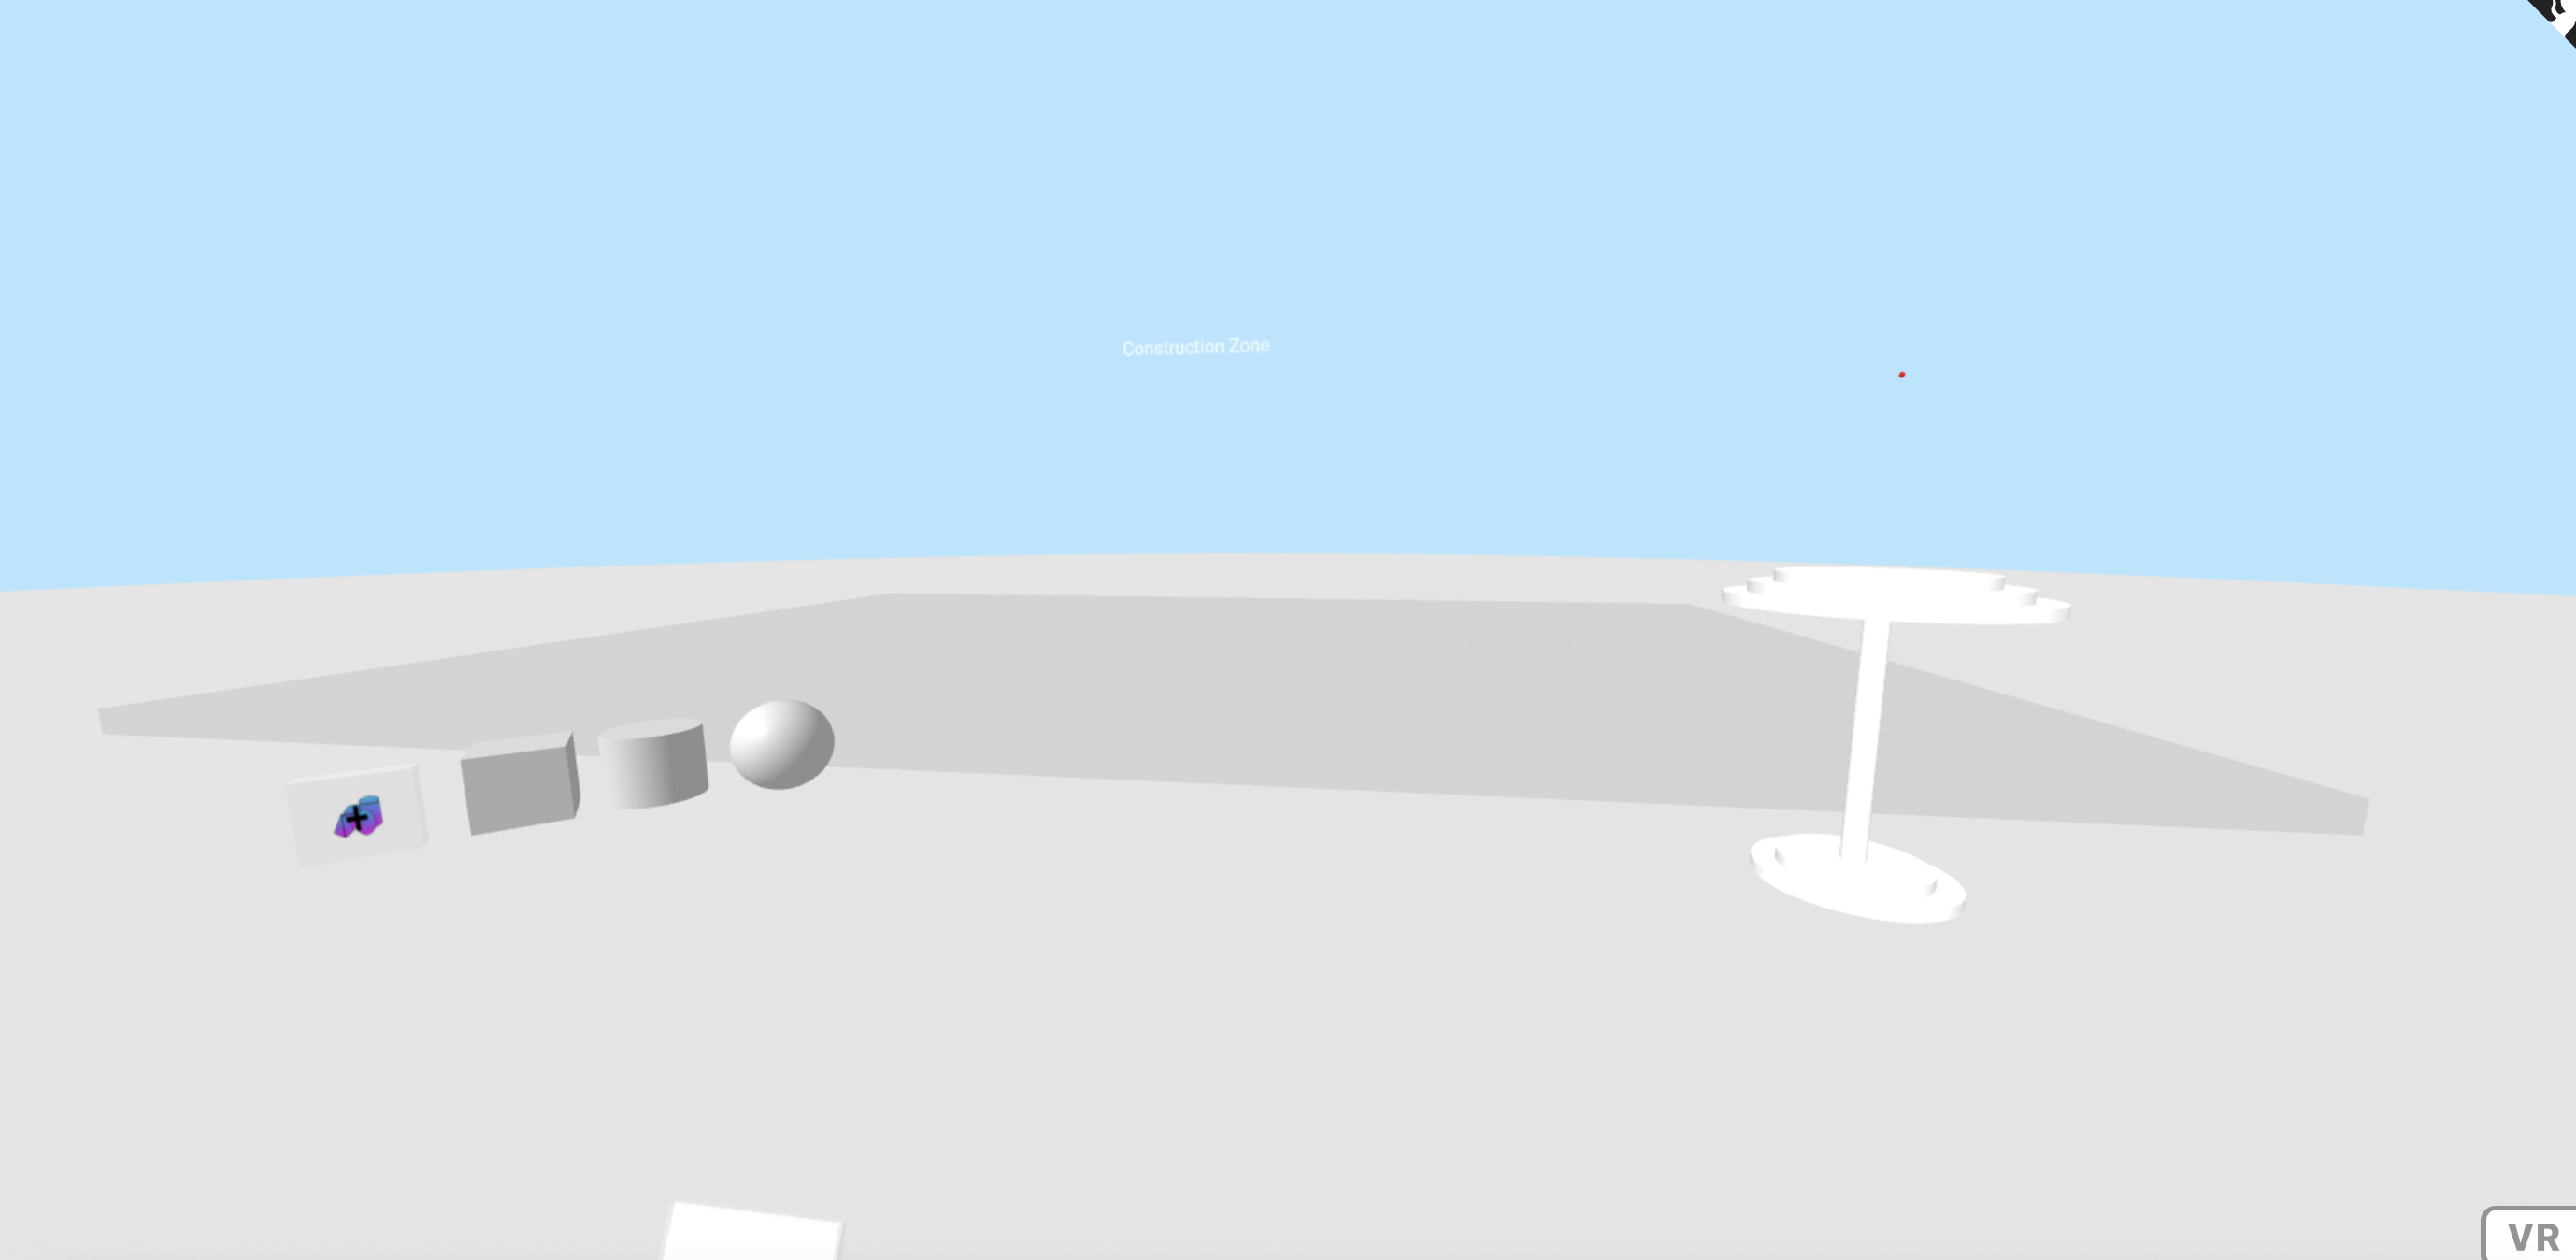
\includegraphics[width=9cm, keepaspectratio]{MemoriaTFG-JulianPerez/img/gen.png}
  \caption{Escenario general}\label{gen}
\end{figure}

Las figuras que sean clicables se verá mas claro que se pueden clicar.
\begin{figure}[H]
  \centering
  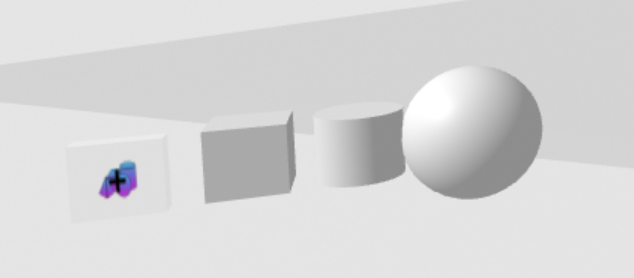
\includegraphics[width=7cm, keepaspectratio]{MemoriaTFG-JulianPerez/img/figs.png}
  \caption{Figura seleccionada}\label{scrum}
\end{figure}

Respecto al menú de creación de figuras y el modo grupo, haré que sigan al usuario para se encuentre de una manera más accesible y escondida y de este modo, visualizar mejor el escenario. Respecto al menú de las figuras con ayuda de la creación de componentes, lo rediseñaremos para que se muestre de una manera más sencilla y vistosa y le añadiremos la posibilidad de poder esconderlo. También colocaré de una manera más adecuada el menú de modificación de la figura. 

\begin{figure}[H]
  \centering
  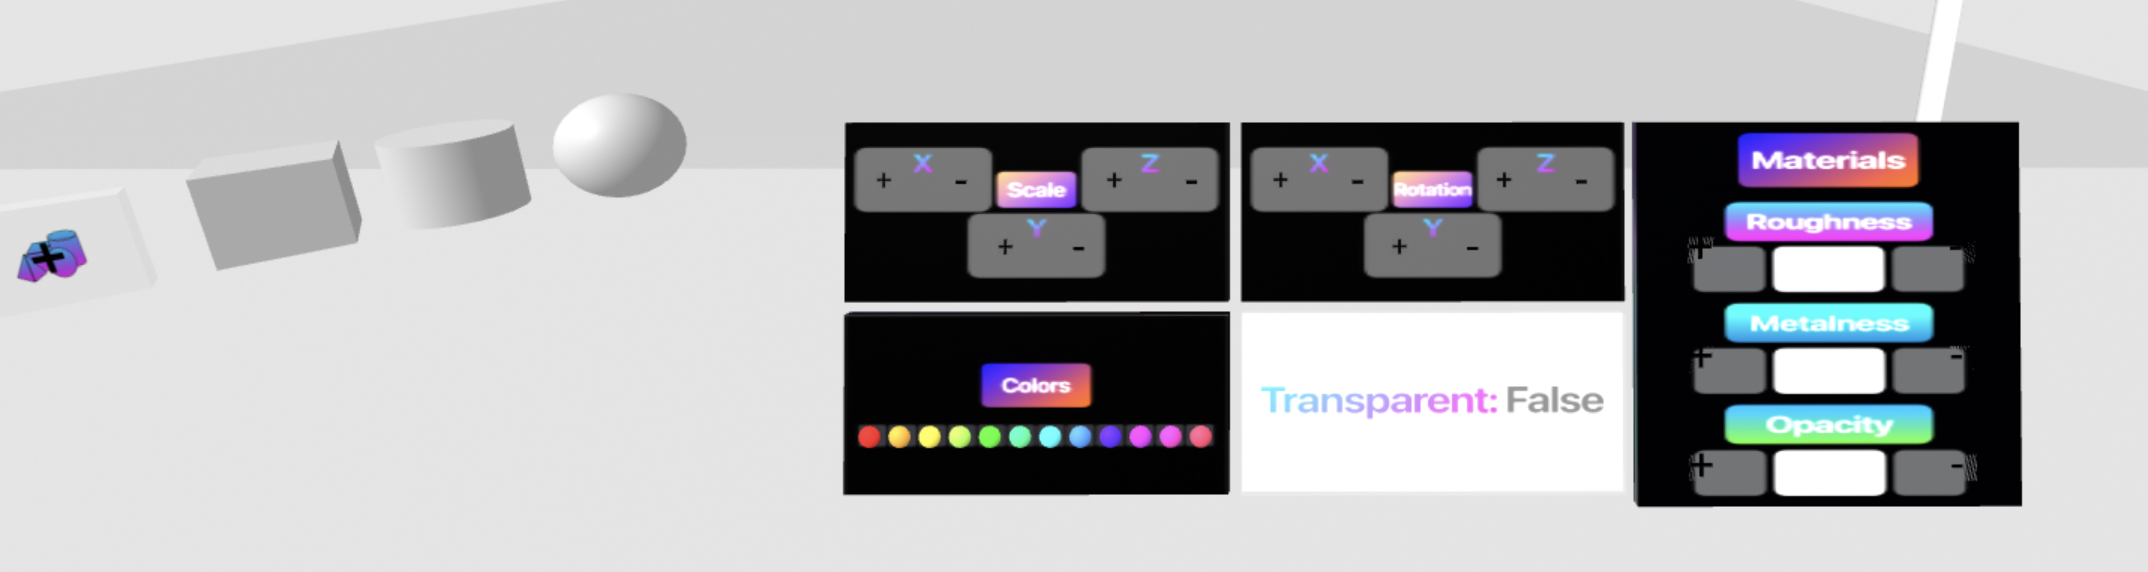
\includegraphics[width=10cm, keepaspectratio]{MemoriaTFG-JulianPerez/img/menu.png}
  \caption{Menú modificación figura}\label{scrum}
\end{figure}

Respecto al modo grupo cambiaré varias cosas, la primera, el manejador ahora tiene una imagen especial para así poder diferenciarlo mejor.

\begin{figure}[H]
  \centering
  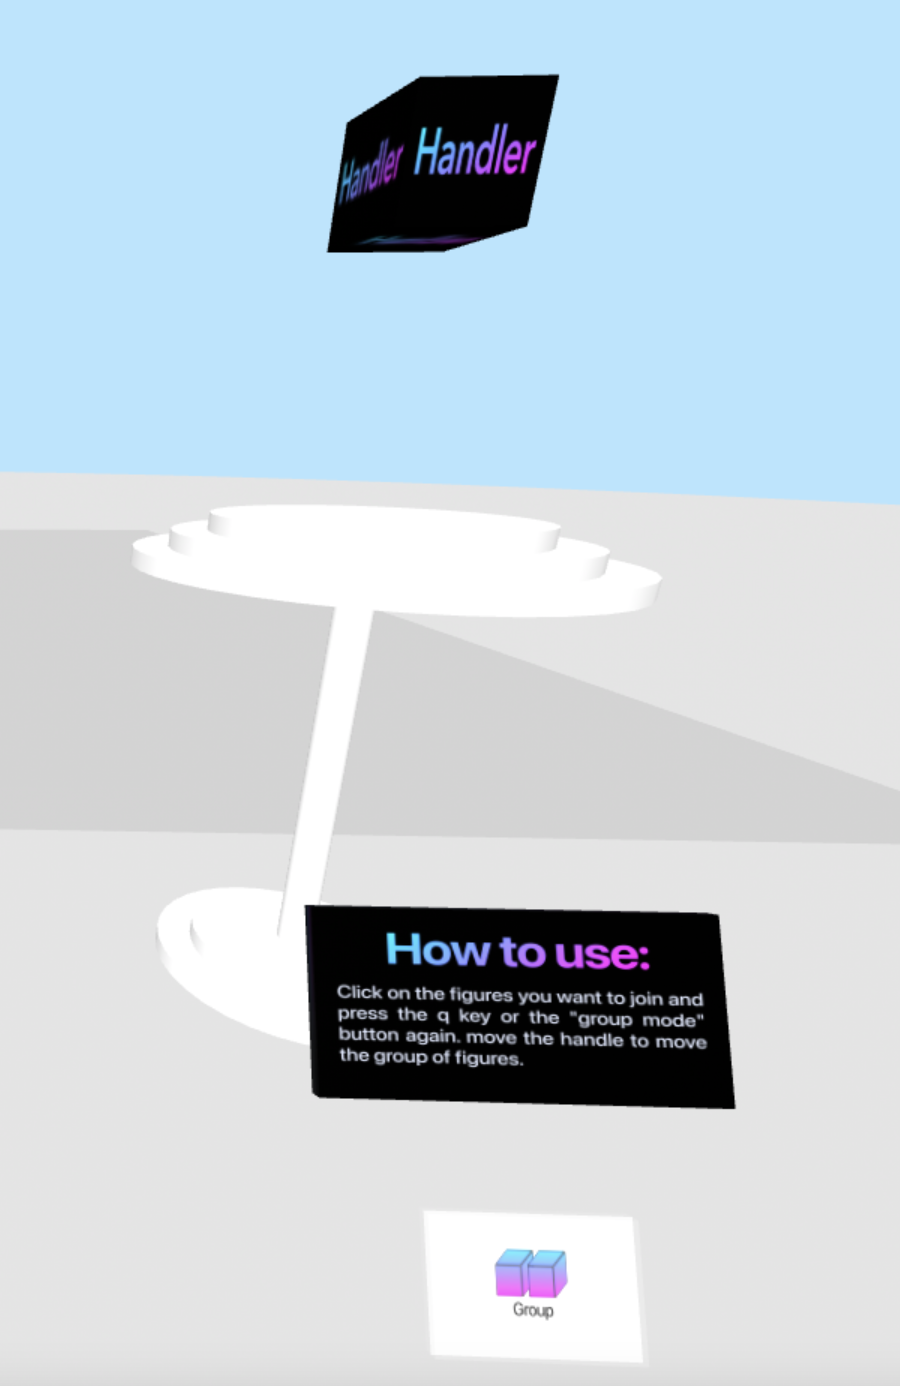
\includegraphics[width=4cm, keepaspectratio]{MemoriaTFG-JulianPerez/img/handler.png}
  \caption{Manejador}\label{scrum}
\end{figure}

Y respecto de las figuras seleccionadas, ahora tendrán una animación al ser clicadas.

\textbf{Tarea 2}

En esta tarea, me centraré en añadir distintas figuras en 3D.

Crearé un menú para estas figuras en las cuales podremos elegir entre distintas figuras las cuales están clasificadas por categorías. Para añadir estas figuras he utilizado el elemento \begin{verbatim} <a-asset-item>\end{verbatim} que nos facilita A-Frame.

El resultado lo podremos observar en el escenario de la manera que nos muestra la figura 3.18

\begin{figure}[H]
  \centering
  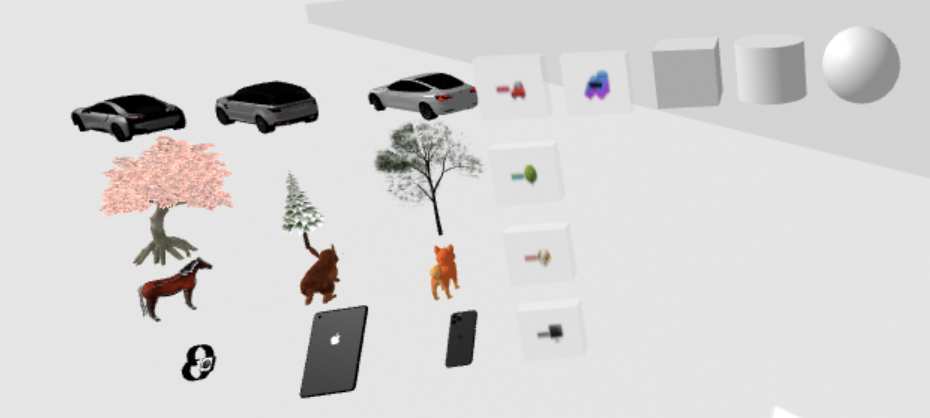
\includegraphics[width=12cm, keepaspectratio]{MemoriaTFG-JulianPerez/img/gltfs.png}
  \caption{Nuevas figuras del editor}\label{fig}
\end{figure}

\textbf{Tarea 3}

En esta tarea añadiré la posibilidad de modificar más propiedades de las figuras.

Con la creación de nuevos componentes se añadió la capacidad de modificar la orientación de la figura en los tres ejes, rugosidad,la metalización y la opacidad a esta última se le añade una funcionalidad especial la cual puede hacer la figura transparente.

El resultado se puede observar en la figura 3.16

\textbf{Tarea 4}

Por ultimo me centraré en la compatibilidad de nuestro escenario con la gafas de realidad virtual, en concreto, las Oculus Quest. 

\subsection{Resultado}

Como resultado de este sprint, puedo decir que estoy más cerca de la versión final. Solo nos quedaría refinar algunos aspectos. He conseguido crear nuevas funcionalidades, mejorar nuestra aplicación y hacerla más usable para el usuario. Este sprint está disponible en el repositorio del proyecto, tanto el código \footnote{\url{https://github.com/julianperezm/A-frame/tree/master/SeventhExercise}} como el escenario, ya sea la versión escritorio \footnote{\url{https://julianperezm.github.io/A-frame/SeventhExercise/Desktop.html}} o la versión de realidad virtual \footnote{\url{https://julianperezm.github.io/A-frame/SeventhExercise/Glasses.html}}

\section{Sprint Final}
En este sprint me centraré en el final del proyecto puliendo los últimos detalles y añadiendo las ultimas funcionalidades de la aplicación. Acercándolo lo más posible a un editor usable y también lo más atractivo posible.

\subsection{Objetivo}
Los objetivos de este sprint serán:
\begin{itemize}
    \item Seguir mejorando la interfaz de usuario haciéndolo más intuitivo
    \item Añadir nuevos ambientes al editor.
\end{itemize}

\subsection{Desarrollo}
Seguiremos dividiendo las el desarrollo del sprint en tareas.

\textbf{Tarea 1}

En este tarea seguiré mejorando la interfaz de usuario para hacerla más intuitiva y sencilla para el usuario, añadiremos nuevos atributos, como son el porcentaje de progreso de las modificaciones de los materiales que se les pueden realizar a las figuras.

\begin{figure}[H]
  \centering
  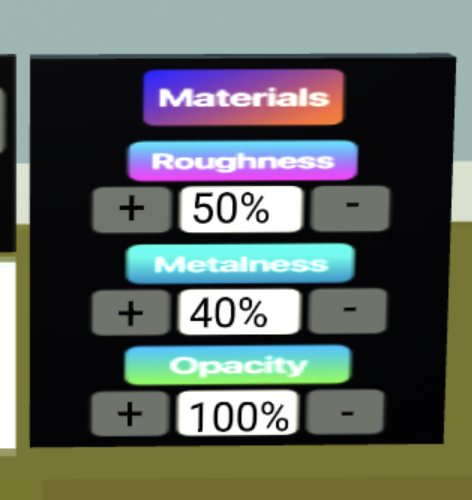
\includegraphics[width=6cm, keepaspectratio]{MemoriaTFG-JulianPerez/img/menu2.png}
  \caption{Nuevo menú de propiedades}\label{menu2}
\end{figure}

También añadiré una luz en el pódium para que las modificaciones que le hacemos a la figura se puedan visualizar de una manera más clara.

\begin{figure}[H]
  \centering
  \begin{minipage}[b]{0.4\textwidth}
 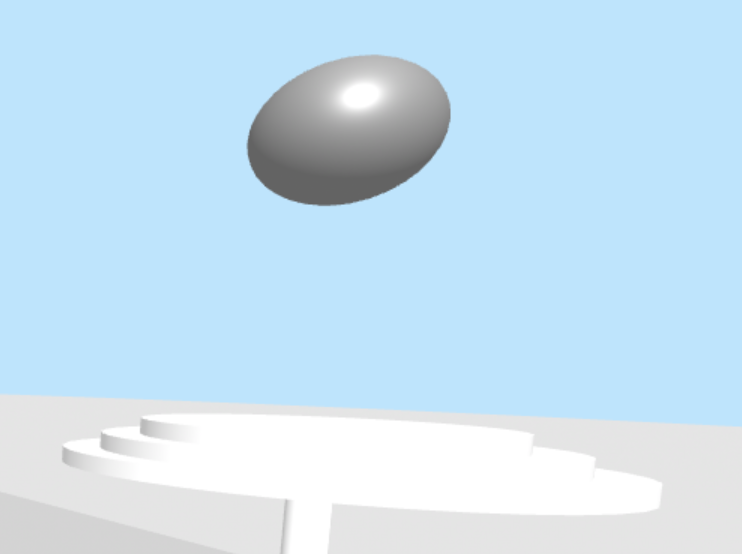
\includegraphics[width=7cm]{MemoriaTFG-JulianPerez/img/sinluz.png}
  \caption{Podium sin luz}\label{single}
  \end{minipage}
  \hfill
  \begin{minipage}[b]{0.4\textwidth}
  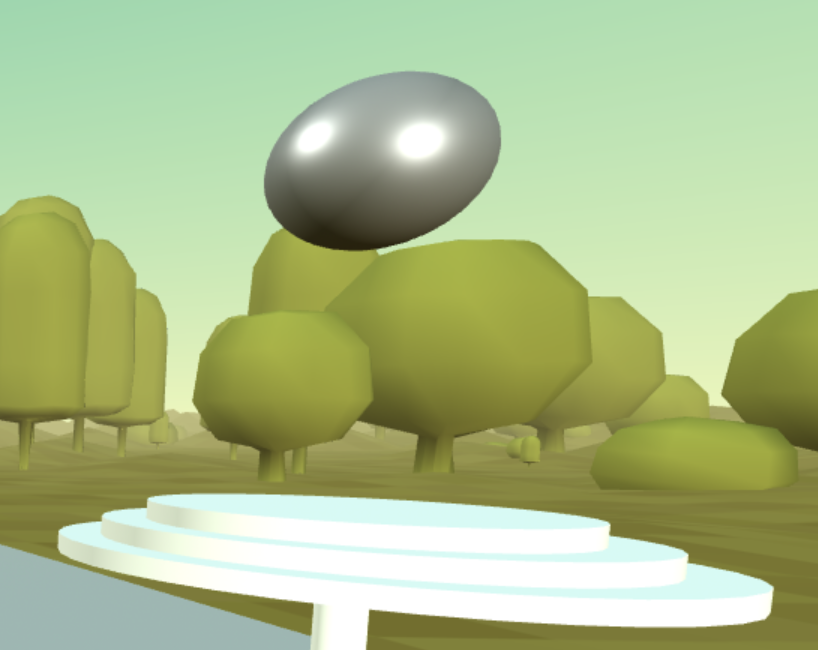
\includegraphics[width=7cm]{MemoriaTFG-JulianPerez/img/luz.png}
  \caption{Podium con luz}\label{scrum}
  \end{minipage}
\end{figure}

\textbf{Tarea 2}

En esta tarea me centraré en mejorar la funcionalidad de modo grupo, añadiremos un botón para así poder eliminar el manejador y el escenario quede mucho mas limpio.

Además de esta mejora añadiremos una funcionalidad la cual te permita cambiar de ambiente al escenario.

La eliminación de los manejadores es posible añadiendo un componente que añada opacidad a dichas figuras. el escenario con manejadores quedaría como muestra la figura 3.22 y sin manejadores como la figura 3.23.

\begin{figure}[H]
  \centering
  \begin{minipage}[b]{0.4\textwidth}
 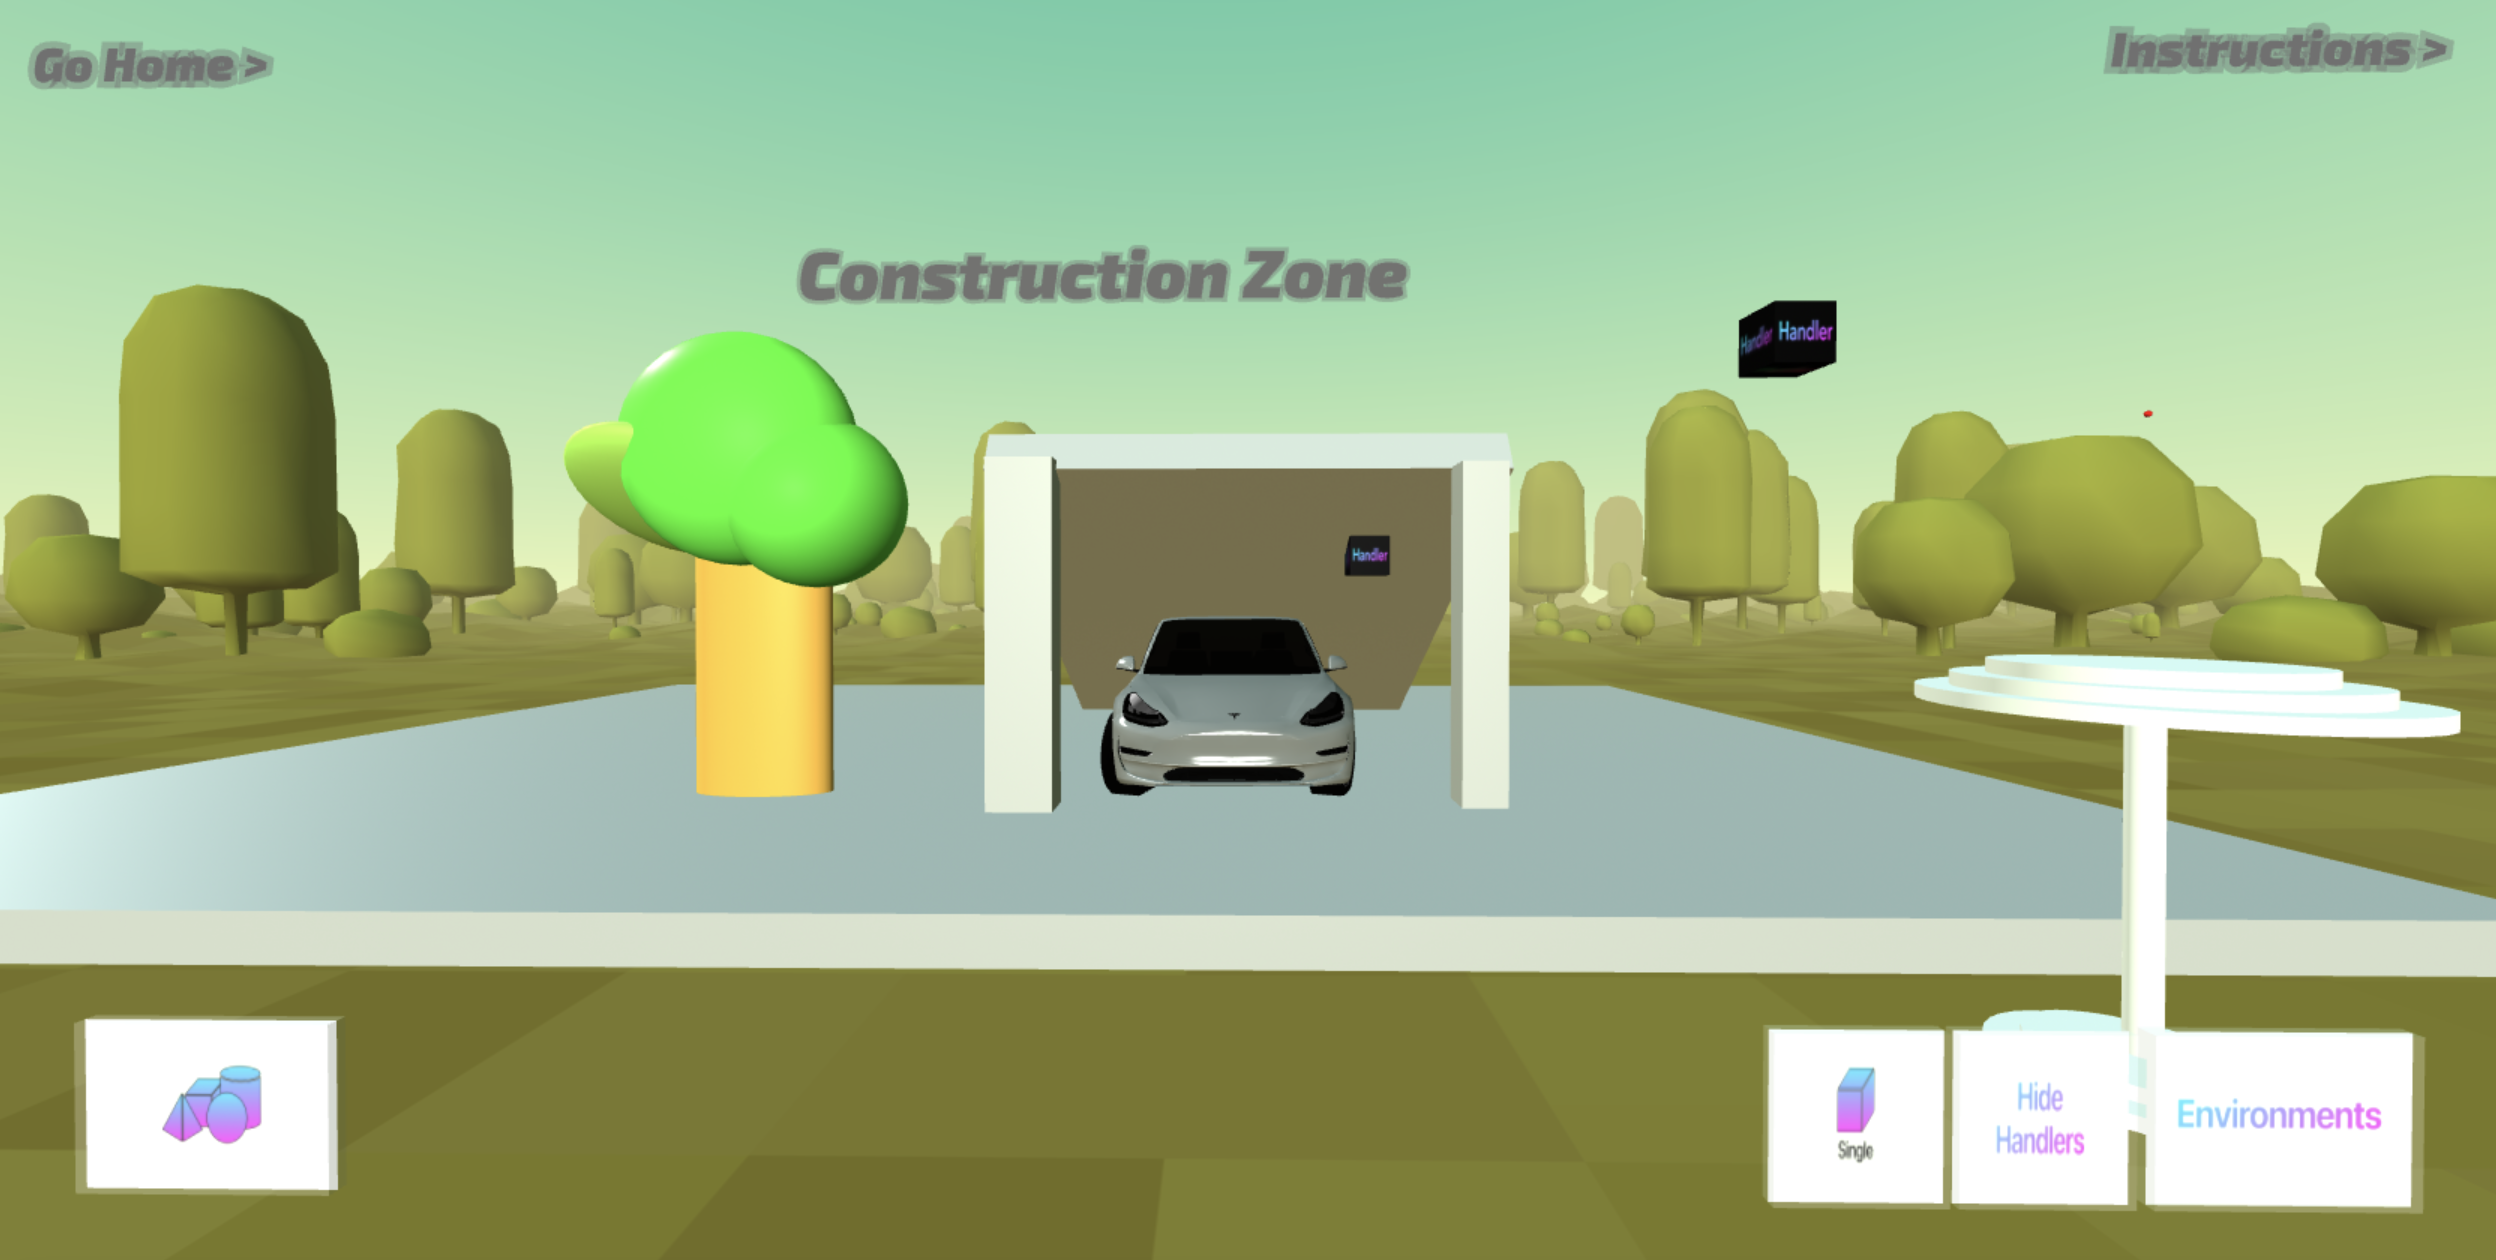
\includegraphics[width=7cm]{MemoriaTFG-JulianPerez/img/conm.png}
  \caption{Escenario con manejadores}\label{single}
  \end{minipage}
  \hfill
  \begin{minipage}[b]{0.4\textwidth}
  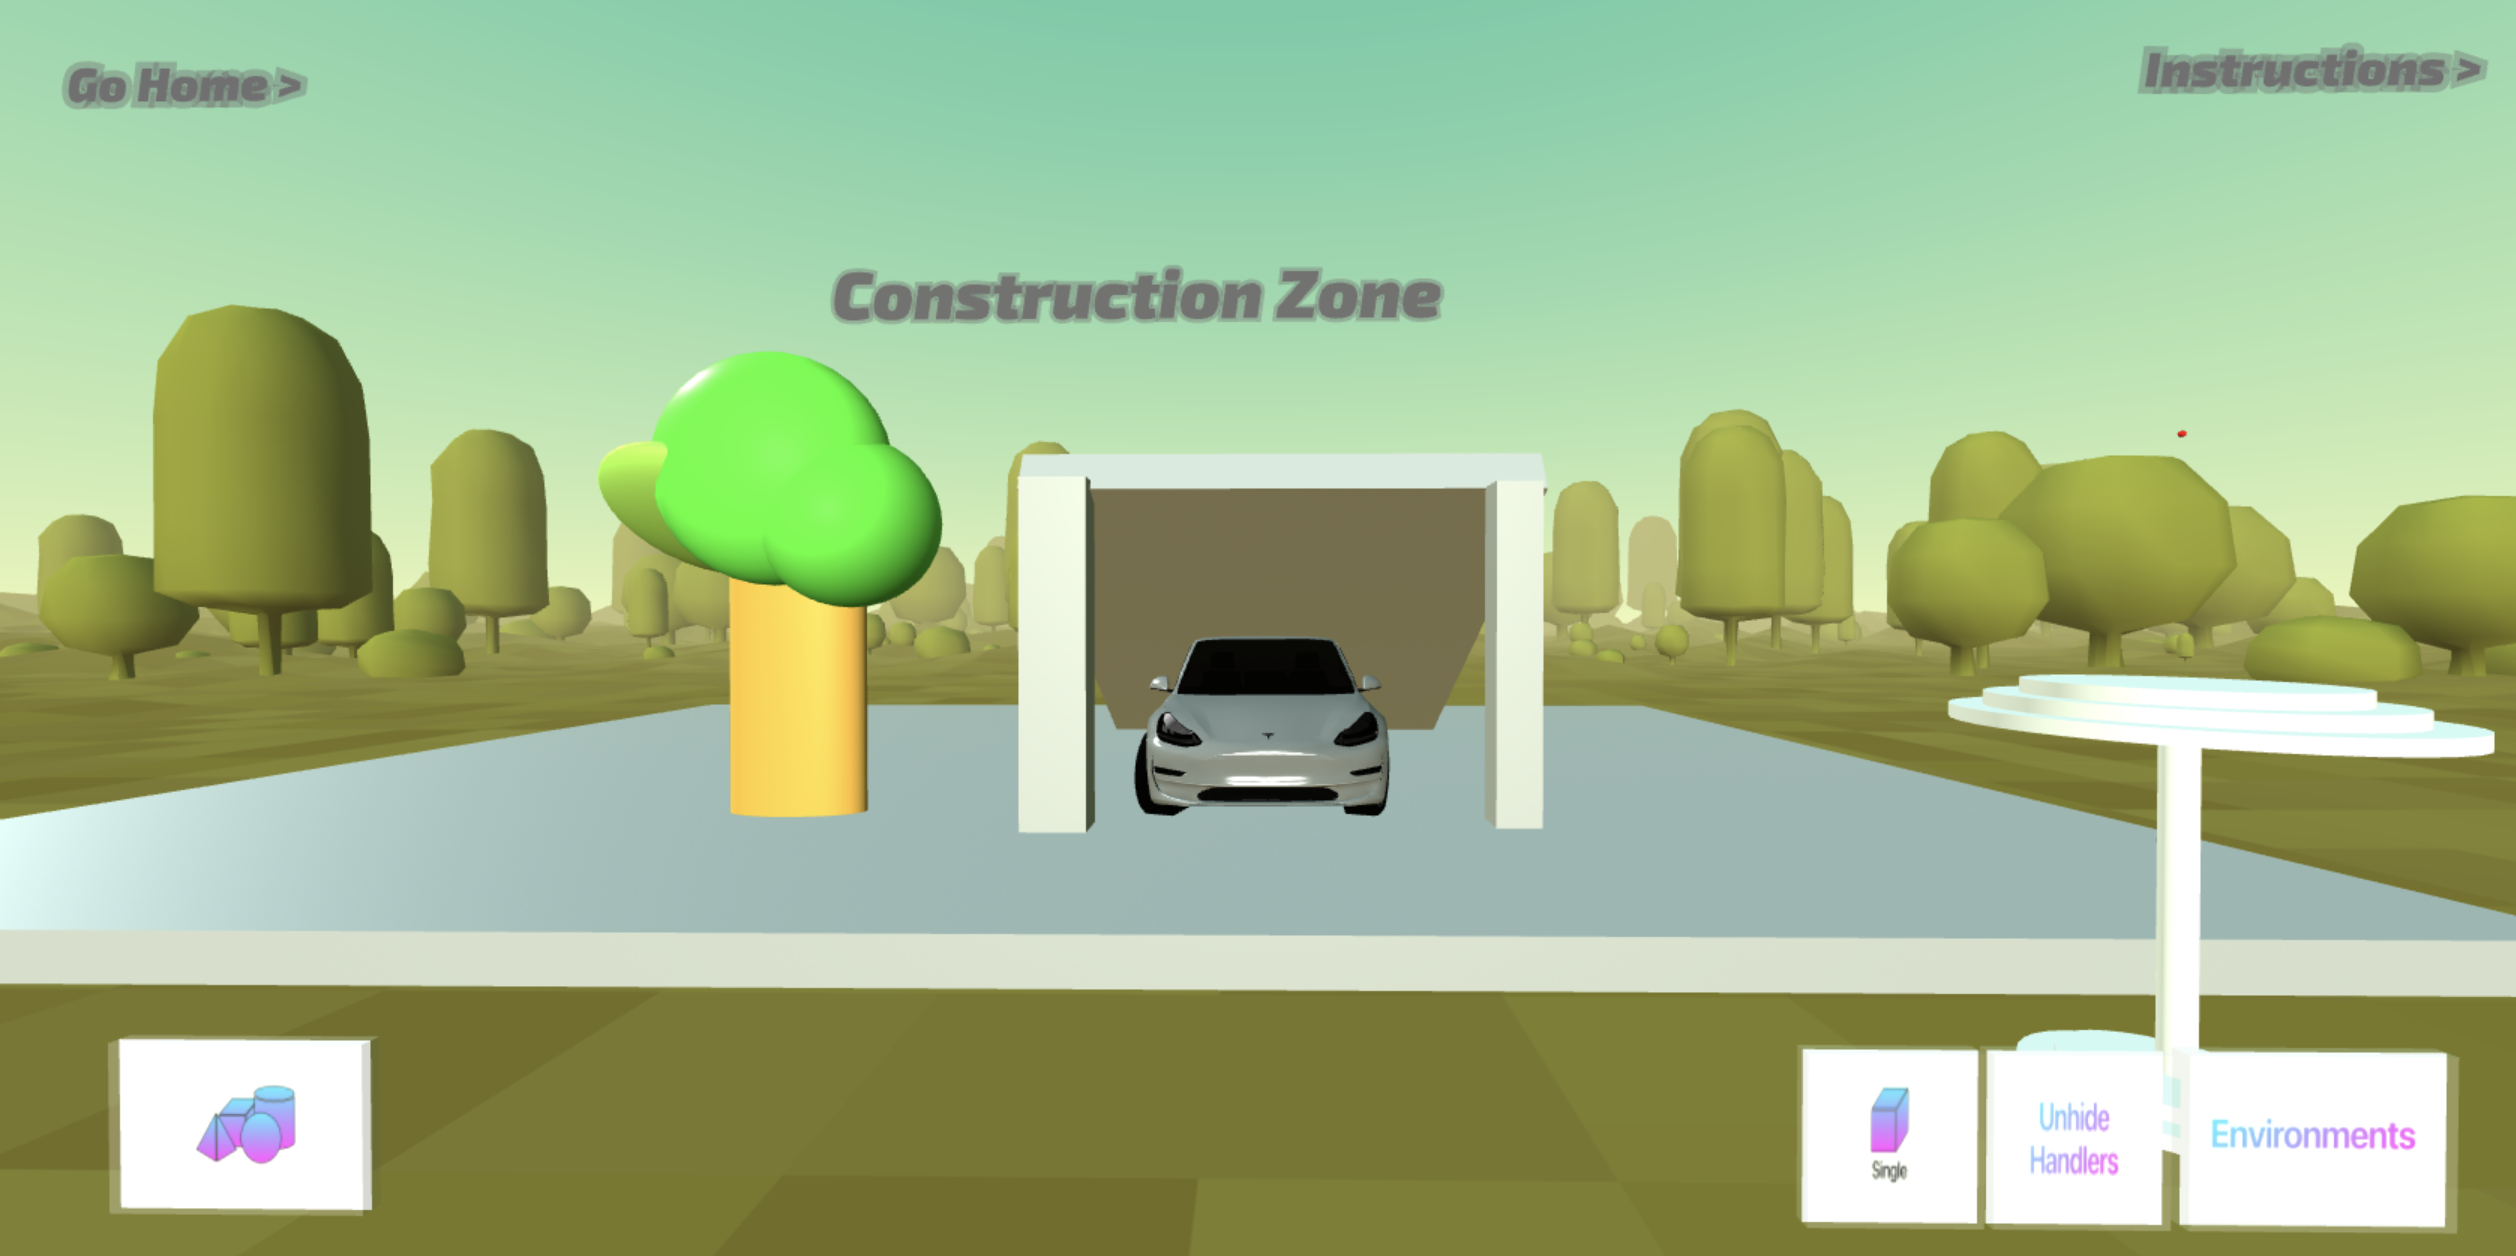
\includegraphics[width=7cm]{MemoriaTFG-JulianPerez/img/sinm.png}
  \caption{Escenario sin manejadores}\label{scrum}
  \end{minipage}
\end{figure}

Para los cambios de ambientes utilizaré un componente creado por la comunidad, se puede encontrar en su repositorio de GitHub \footnote{\url{https://github.com/supermedium/aframe-environment-component}}. 

El resultado de esta parte de la tarea se puede visualizar en la escena con un desplegable en el que puedes elegir que ambiente usar como se muestra en la figura 3.24.

\begin{figure}[H]
  \centering
  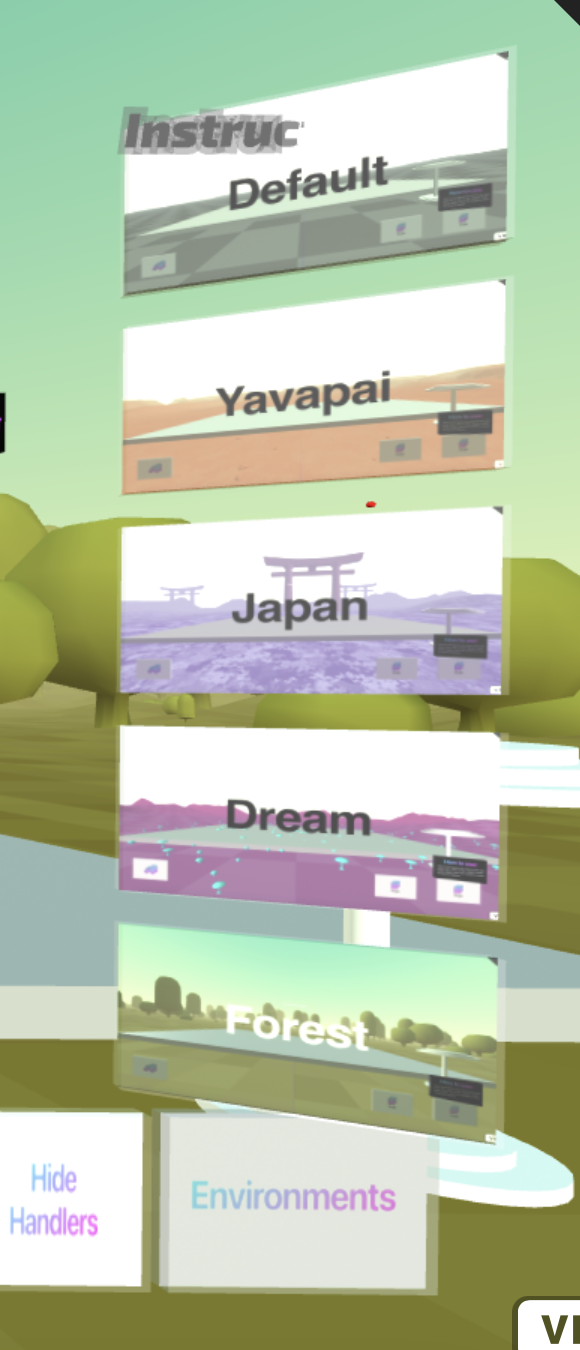
\includegraphics[width=4cm, keepaspectratio]{MemoriaTFG-JulianPerez/img/env.png}
  \caption{Menú de ambientes}\label{menu2}
\end{figure}

\textbf{Tarea 3}

Esta última tarea tratará de terminar la aplicación añadiéndole una página principal,

\begin{figure}[H]
  \centering
  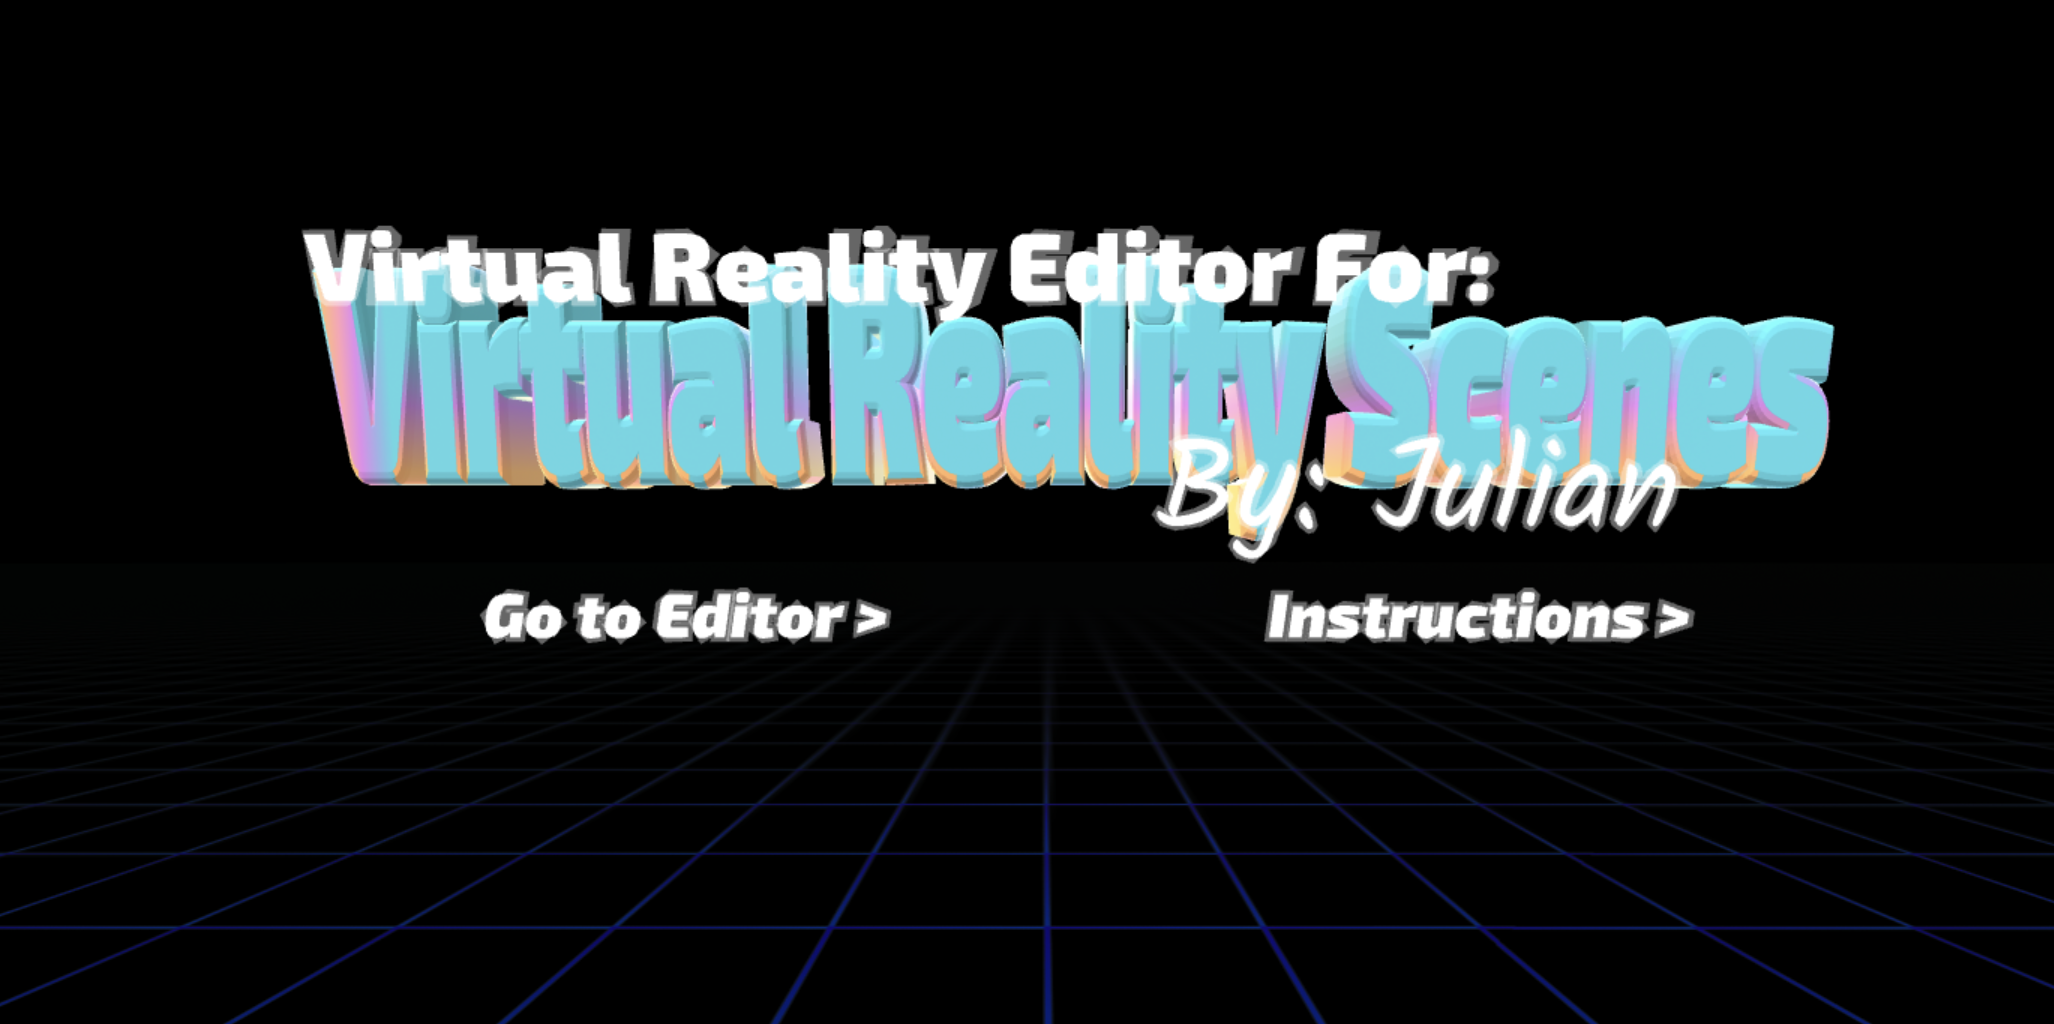
\includegraphics[width=10cm, keepaspectratio]{MemoriaTFG-JulianPerez/img/home.png}
  \caption{Página de inicio}\label{home}
\end{figure}

y otra página de instrucciones.

\begin{figure}[H]
  \centering
  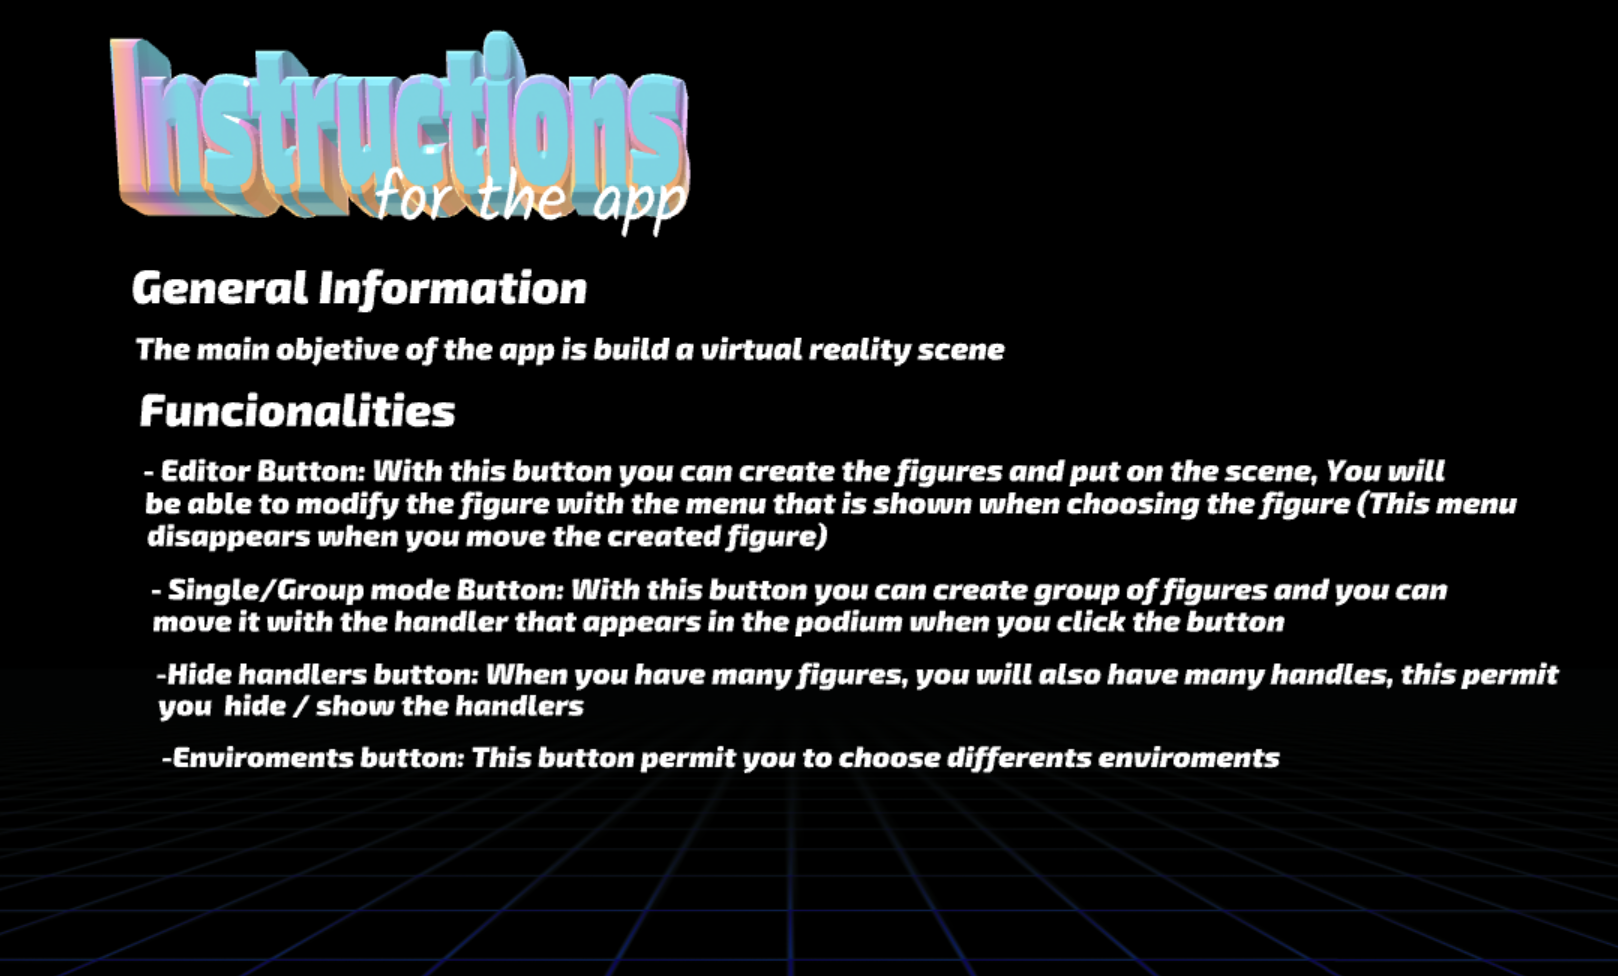
\includegraphics[width=10cm, keepaspectratio]{MemoriaTFG-JulianPerez/img/inst.png}
  \caption{Página de instrucciones}\label{home}
\end{figure}

Amabas son accesibles entre ellas además del escenario.

\subsection{Resultado}

En este último sprint he conseguido terminar el proyecto, este proyecto puede seguir desarrollándose y mejorando, puede ser el comienzo de algo grande. El código \footnote{\url{https://github.com/julianperezm/A-frame/tree/master/Home}}.  y el escenario, ya sea la versión escritorio \footnote{\url{https://julianperezm.github.io/A-frame/Home/HomeDesktop.html}} o la versión compatible con las gafas \footnote{\url{https://julianperezm.github.io/A-frame/Home/HomeGlasses.html}} están disponibles en el repositorio del proyecto en GitHub.

%%%%%%%%%%%%%%%%%%%%%%%%%%%%%%%%%%%%%%%%%%%%%%%%%%%%%%%%%%%%%%%%%%%%%%%%%%%%%%%%
%%%%%%%%%%%%%%%%%%%%%%%%%%%%%%%%%%%%%%%%%%%%%%%%%%%%%%%%%%%%%%%%%%%%%%%%%%%%%%%%
% DISEÑO E IMPLEMENTACIÓN %
%%%%%%%%%%%%%%%%%%%%%%%%%%%%%%%%%%%%%%%%%%%%%%%%%%%%%%%%%%%%%%%%%%%%%%%%%%%%%%%%

\cleardoublepage
\chapter{Resultados}

En esta sección incluiré el manual de usuario de la aplicación donde se mostrará  desde un punto de vista del usuario y de  manera sencilla como utilizar la aplicación y la arquitectura en la que se basa el proyecto donde explicaremos la estructura y los componentes usados para la creación de la aplicación.

\section{Manual de usuario} 
\label{sec:manual de usuario}

Existen dos tipos de interacción del usuario con el escenario, según en que modo de escenario se encuentre, modo escritorio desde la web desde tu ordenador  o inmerso en la propia realidad virtual.

Centrándonos en el modo escritorio, la forma de interactuar con los elementos de la escena se realiza clicando en ellos, para el movimiento de la cámara se utilizará el ratón y para el movimiento del propio usuario se hará uso de las teclas W, A, S, D o de los cursores del teclado. 

Si por el contrario usamos la aplicación con las gafas de realidad virtual, la forma de interactuar con los elementos será con los mandos de estas, el movimiento de la cámara dependerá de donde mire el usuario y  para el movimiento del usuario usaremos el joystick de uno de los mandos o con el propio movimiento del mismo.

Todo comienza en la escena principal, en la cual se puede acceder tanto al editor como a la escena donde puedes ver las instrucciones de la aplicación.

Si accedemos a la pagina de instrucciones el usuario se verá inmerso en una escena, podrá moverse por ella y a su vez leer las instrucciones del editor.

Si por el contrario accedemos a la escena de la aplicación, el usuario se encontrará frente a la zona de construcción y con varios botones en la parte inferior de la cámara como se muestra en la figura 4.1. El botón situado más a la izquierda hace referencia al selector de figuras. El siguiente botón siguiendo el orden hacia la derecha, es el que nos permite activar o desactivar el modo grupo. El botón que sigue hacia la derecha nos permite mostrar u ocultar los manejadores, por último nos encontramos con el botón que nos da acceso a los diferentes ambientes que se pueden añadir al escenario.

\begin{figure}[H]
  \centering
  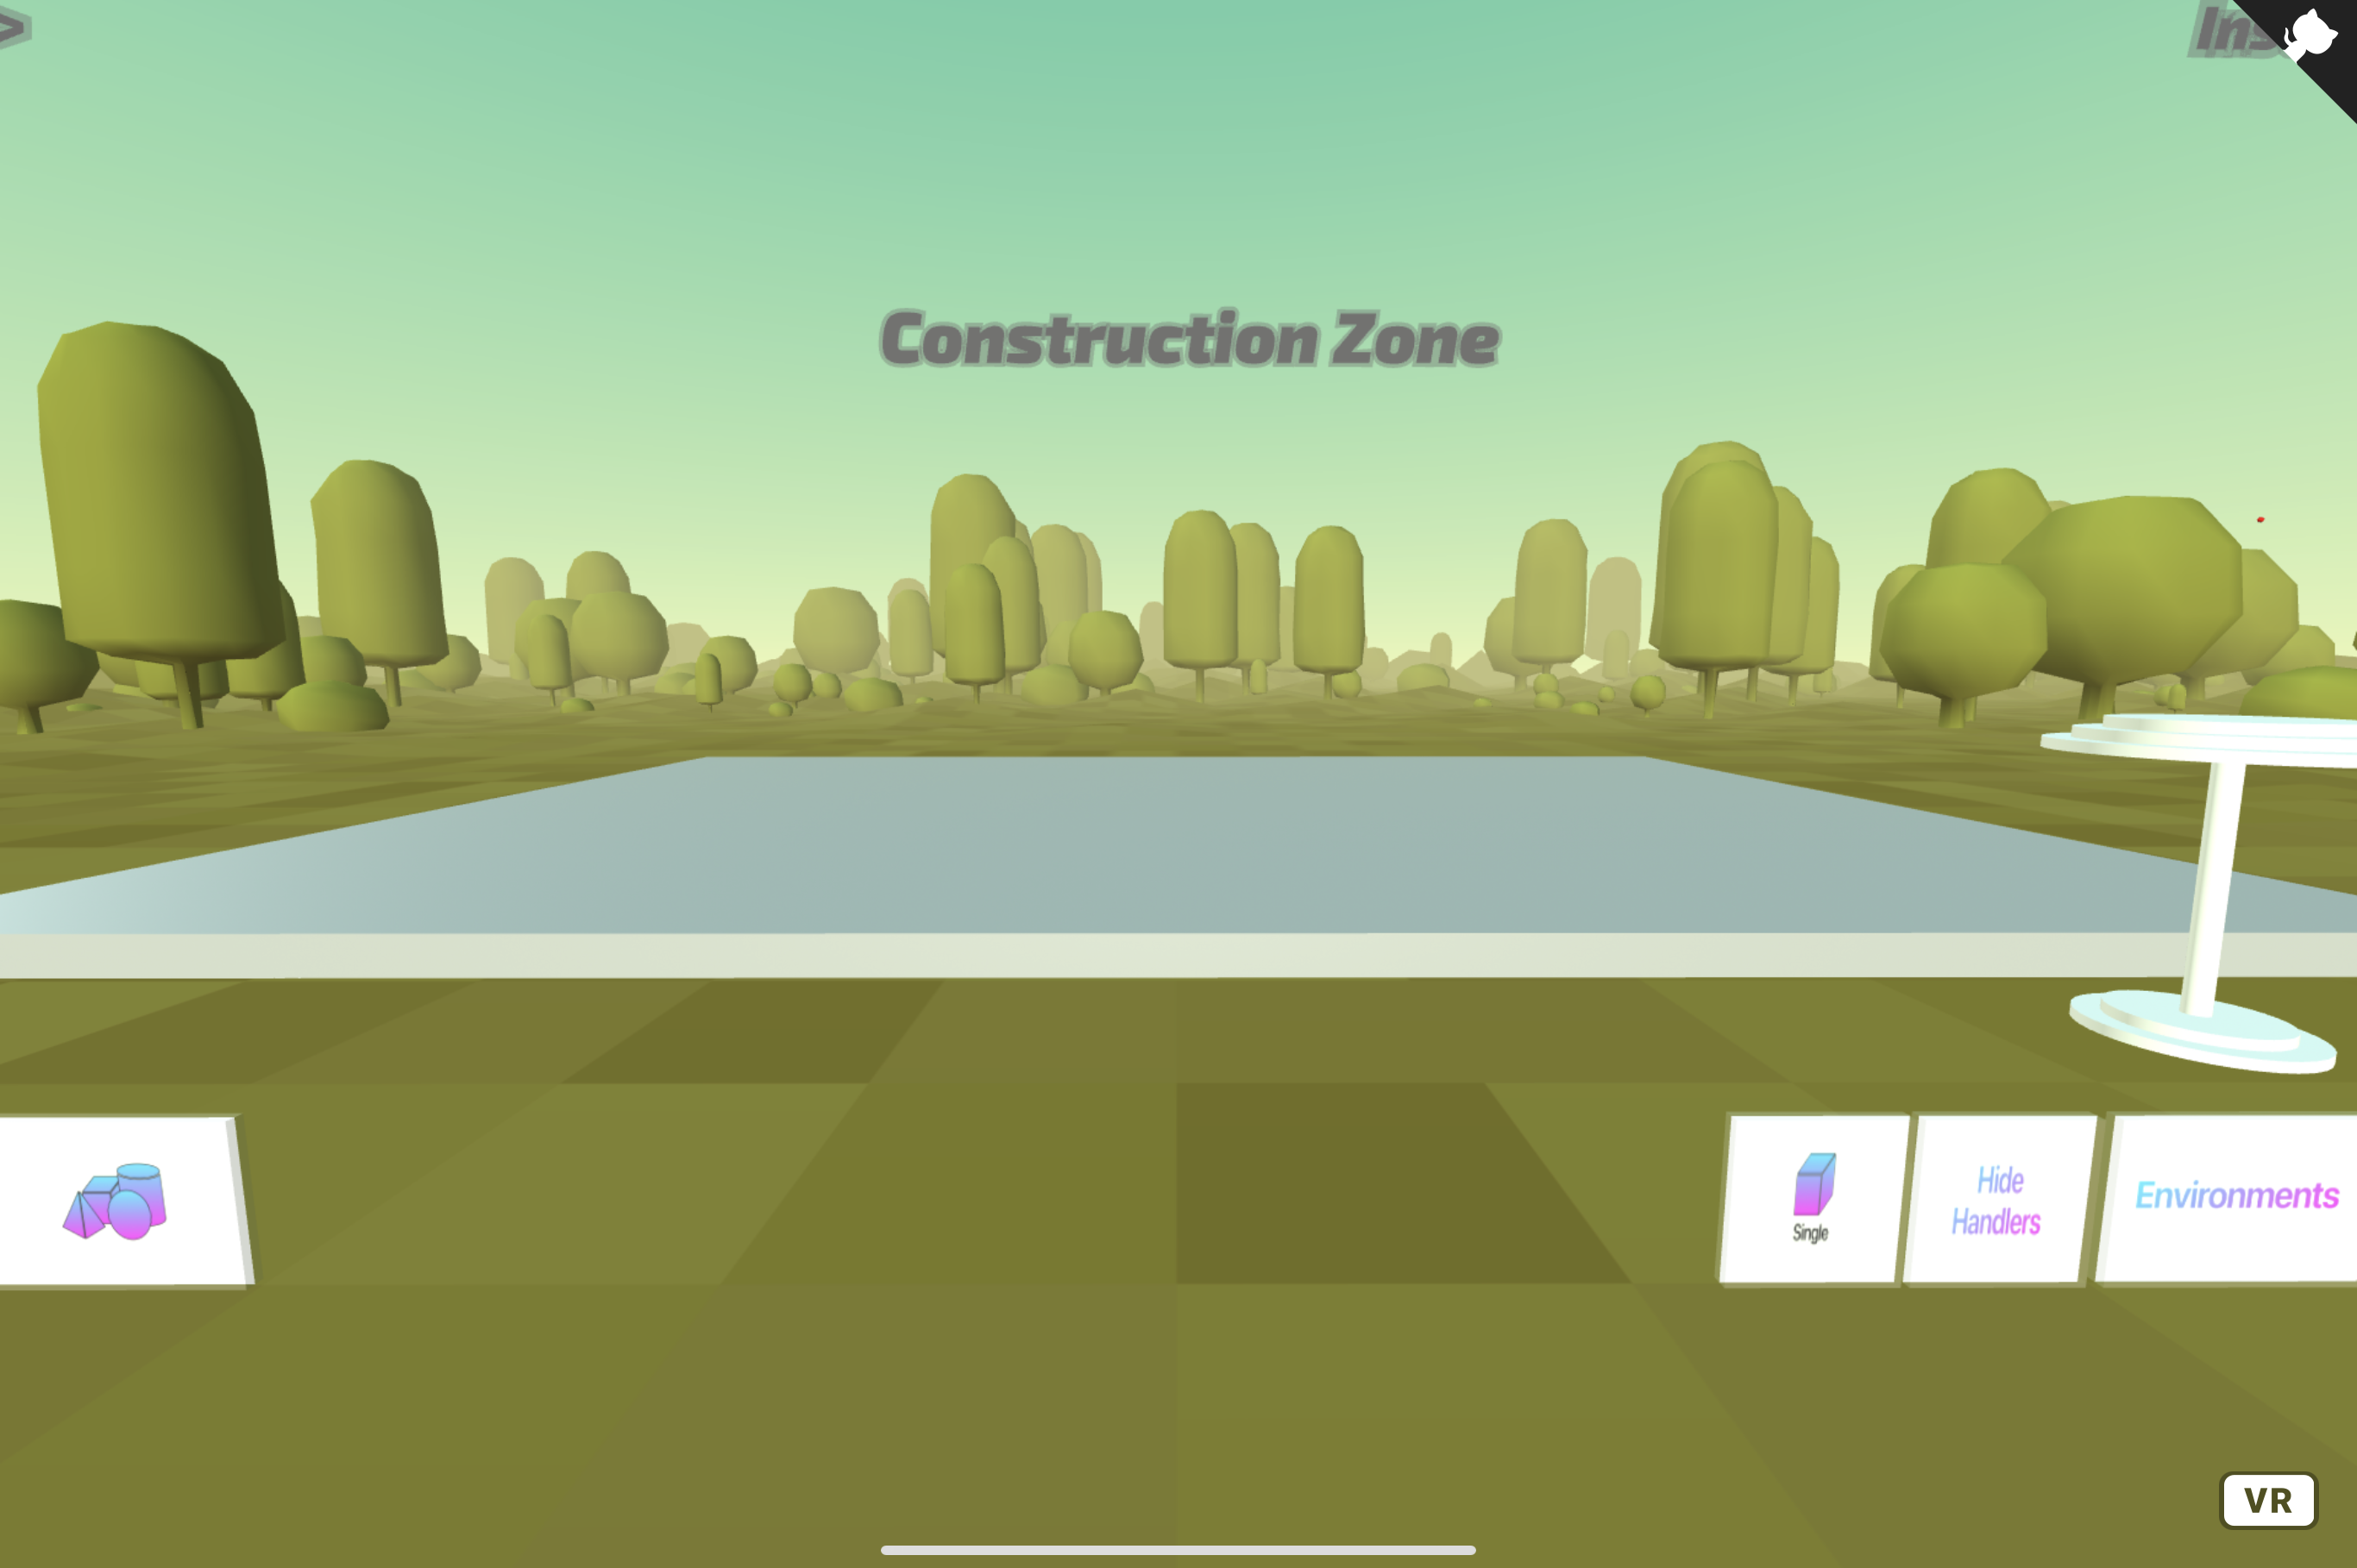
\includegraphics[width=7.7cm, keepaspectratio]{MemoriaTFG-JulianPerez/img/Editor Scene.png}
  \caption{Inicio página del editor}\label{home}
\end{figure}

Si el usuario pulsa el menú de selector de figuras, podrá elegir tanto las figuras básicas como varios modelos 3D, si elegimos uno de estos, aparecerá un menú en el cual, pulsando los botones "+" o "-", podremos modificar dos atributos principales de las figuras, la orientación y el tamaño.

\begin{figure}[H]
  \centering
  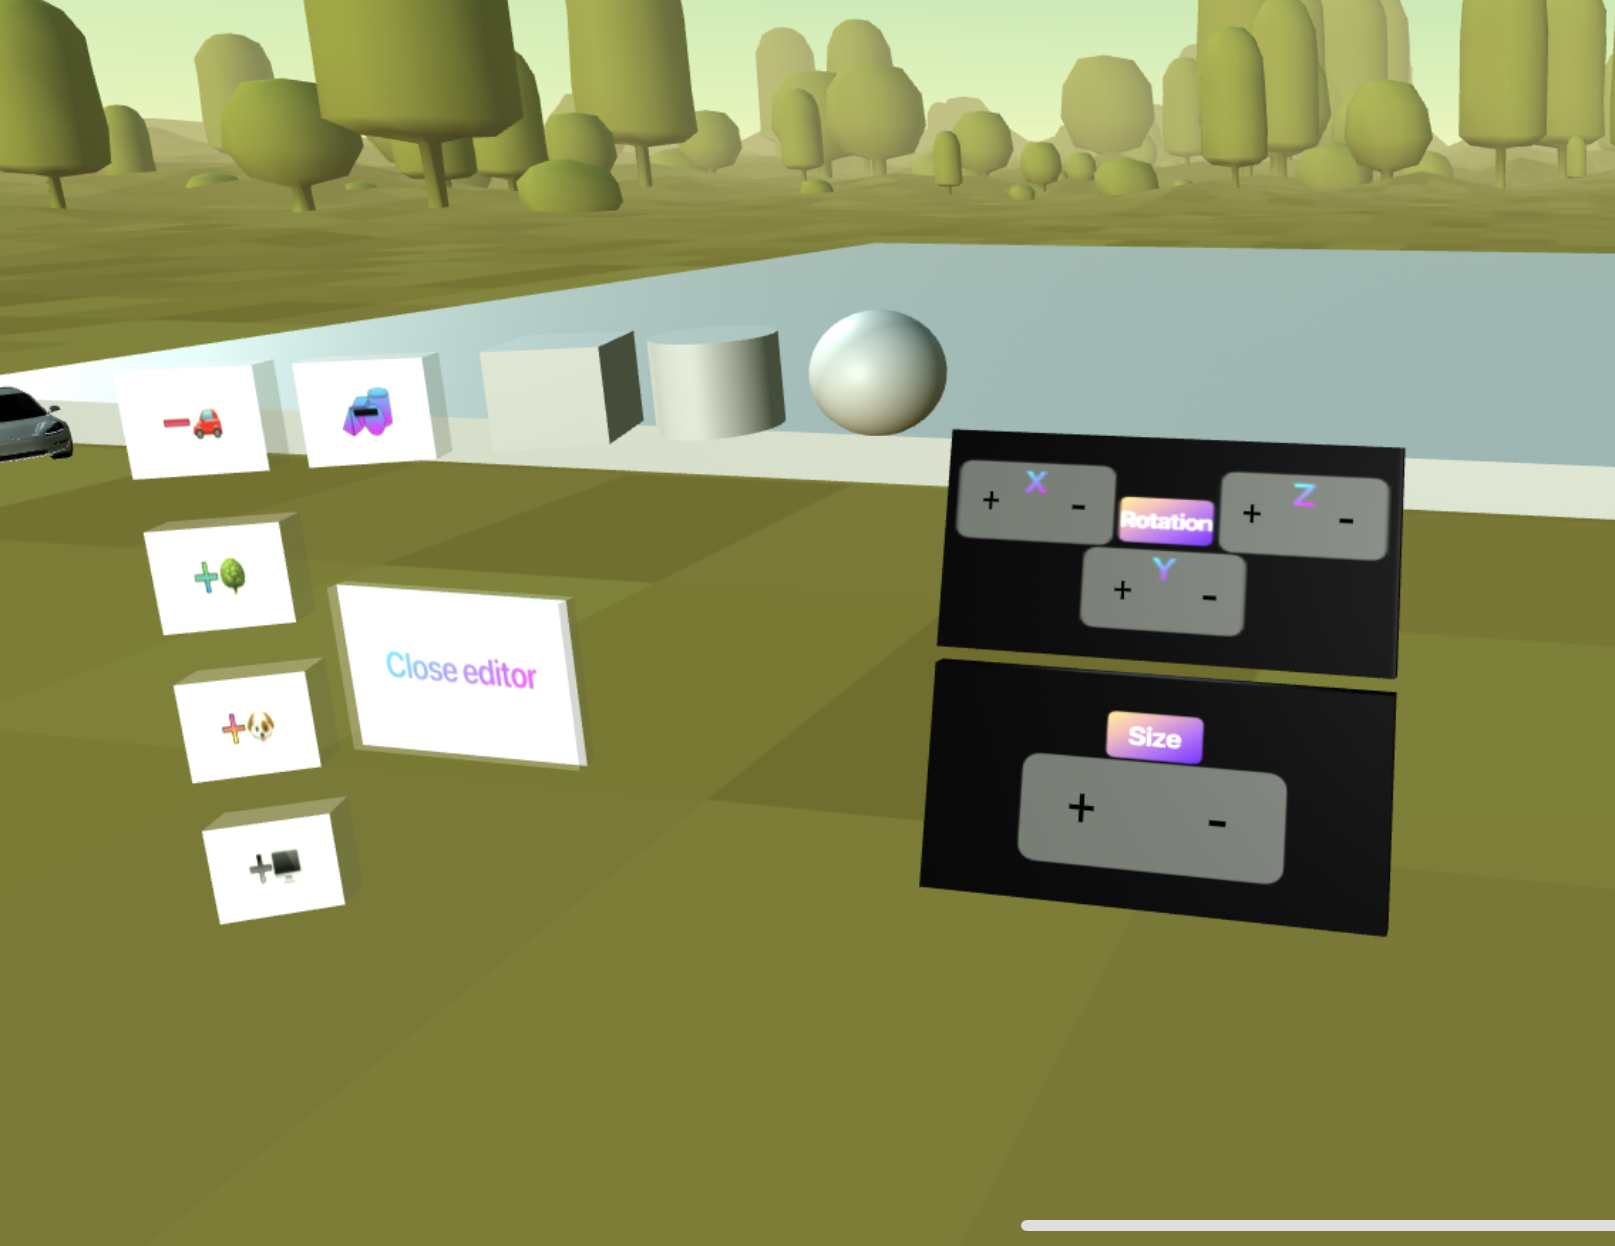
\includegraphics[width=10cm, keepaspectratio]{MemoriaTFG-JulianPerez/img/Screenshot 2021-05-24 at 22.49.26.png}
  \caption{Menú modificación glTFs}\label{home}
\end{figure}

Si el usuario decide pulsar una de las tres figuras básicas, el menú de modificación de la figura se amplia de manera notable, podremos modificarlas del mismo modo que el anteriormente, pulsando los botones + y -, el tamaño, el color, la orientación, la transparencia, opacidad, metalizado y la rugosidad. En la figura 3.16 se puede visualizar dicho menú.

Una vez elegida la figura y las modificaciones correspondientes, la cogeremos del podium y la arrastraremos al lugar deseado del escenario. En la figura 3.20 se muestra como se visualiza la figura en este.

Tras haber creado varias figuras, el usuario podrá crear otra, siendo esta la unión de varias, esto lo puede realizar gracias al modo grupo, a la cual se podrá acceder pulsando en el botón situado más a la izquierda que se muestra en la figura 4.3.
\begin{figure}[H]
  \centering
  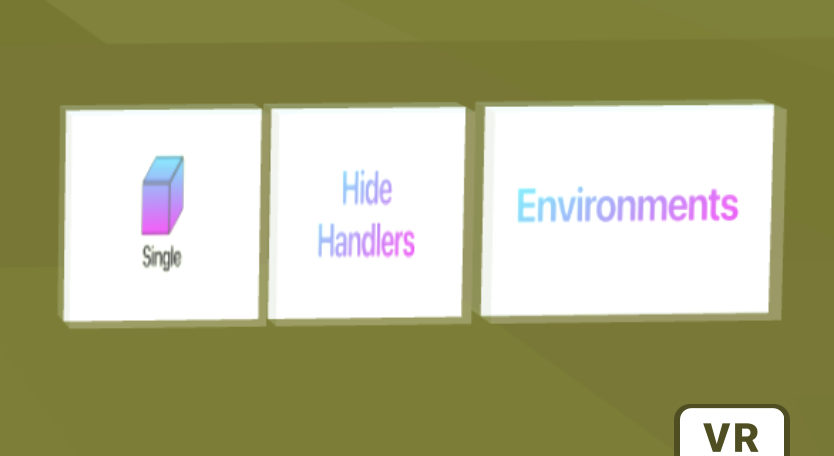
\includegraphics[width=10cm, keepaspectratio]{MemoriaTFG-JulianPerez/img/EditorScene.png}
  \caption{Botones para acceder a las funcionalidades.}\label{home}
\end{figure}

Una vez el modo grupo esté activado, deberás pulsar las figuras que quieres unir, estas realizarán una animación haciendo ver que han sido seleccionadas y una vez ya las tengamos todas, volveremos a pulsar en el botón para confirmar el grupo. Esta figura se moverá mediante el manejador, generado en el podium. Esta funcionalidad puede activarse mediante un atajo de teclado, la tecla Q.

Si se crean muchos grupos de figuras, el escenario estará formado tanto por las propias figuras como por los manejadores, el usuario tendrá el poder de ocultar los manejadores pulsando el botón, 'Hide handler'. Como se observa en la figura 4.3.

La posibilidad de cambiar de ambientes en la escena es posible pulsando botón de menú de ambientes situado a la derecha de la pantalla. En él, nos aparecerán todos los ambientes que podemos elegir. para elegirlos solo tendremos que pulsarlos y el ambiente del escenario cambiará.

Por último en la parte superior tanto izquierda como derecha el usuario se encontrará dos botones mediante los cuales poder acceder tanto a la página de inicio como a la de instrucciones.

\section{Construcción de escenas}
\label{sec:Construcción de escenas}
Gracias a como está construida la aplicación, podemos utilizar los componentes en cualquier otro escenario que no sea el definido para este proyecto.

Para poder empezar a usar la aplicación, lo único que debemos añadir a nuestro código HTML es lo siguiente:

\begin{verbatim}
  <!-- Podium -->
  <a-entity class="podium" podium></a-entity> 
  <!--User Camera-->
  <a-entity>
  <a-box id="showeditor" showeditor></a-box>
  <a-entity id="menu" menu></a-entity>
  <a-entity id="menuenv"></a-entity>
  <a-entity id="editor"></a-entity>
  <a-box id="showhandler" handlereditor></a-box>
  <a-box id="deletehandler" deletehandler></a-box>
  <a-box id="selectenviroments" selectenv></a-box>
  <a-entity gotohome ></a-entity>
  <a-entity gotoinstructiondesktop ></a-entity>
  </a-entity>
\end{verbatim}

Con este código, de ejemplo, ya podrás acceder a todas las funcionalidades de la aplicación como se muestra en la figura 4.4.

\begin{figure}[H]
  \centering
  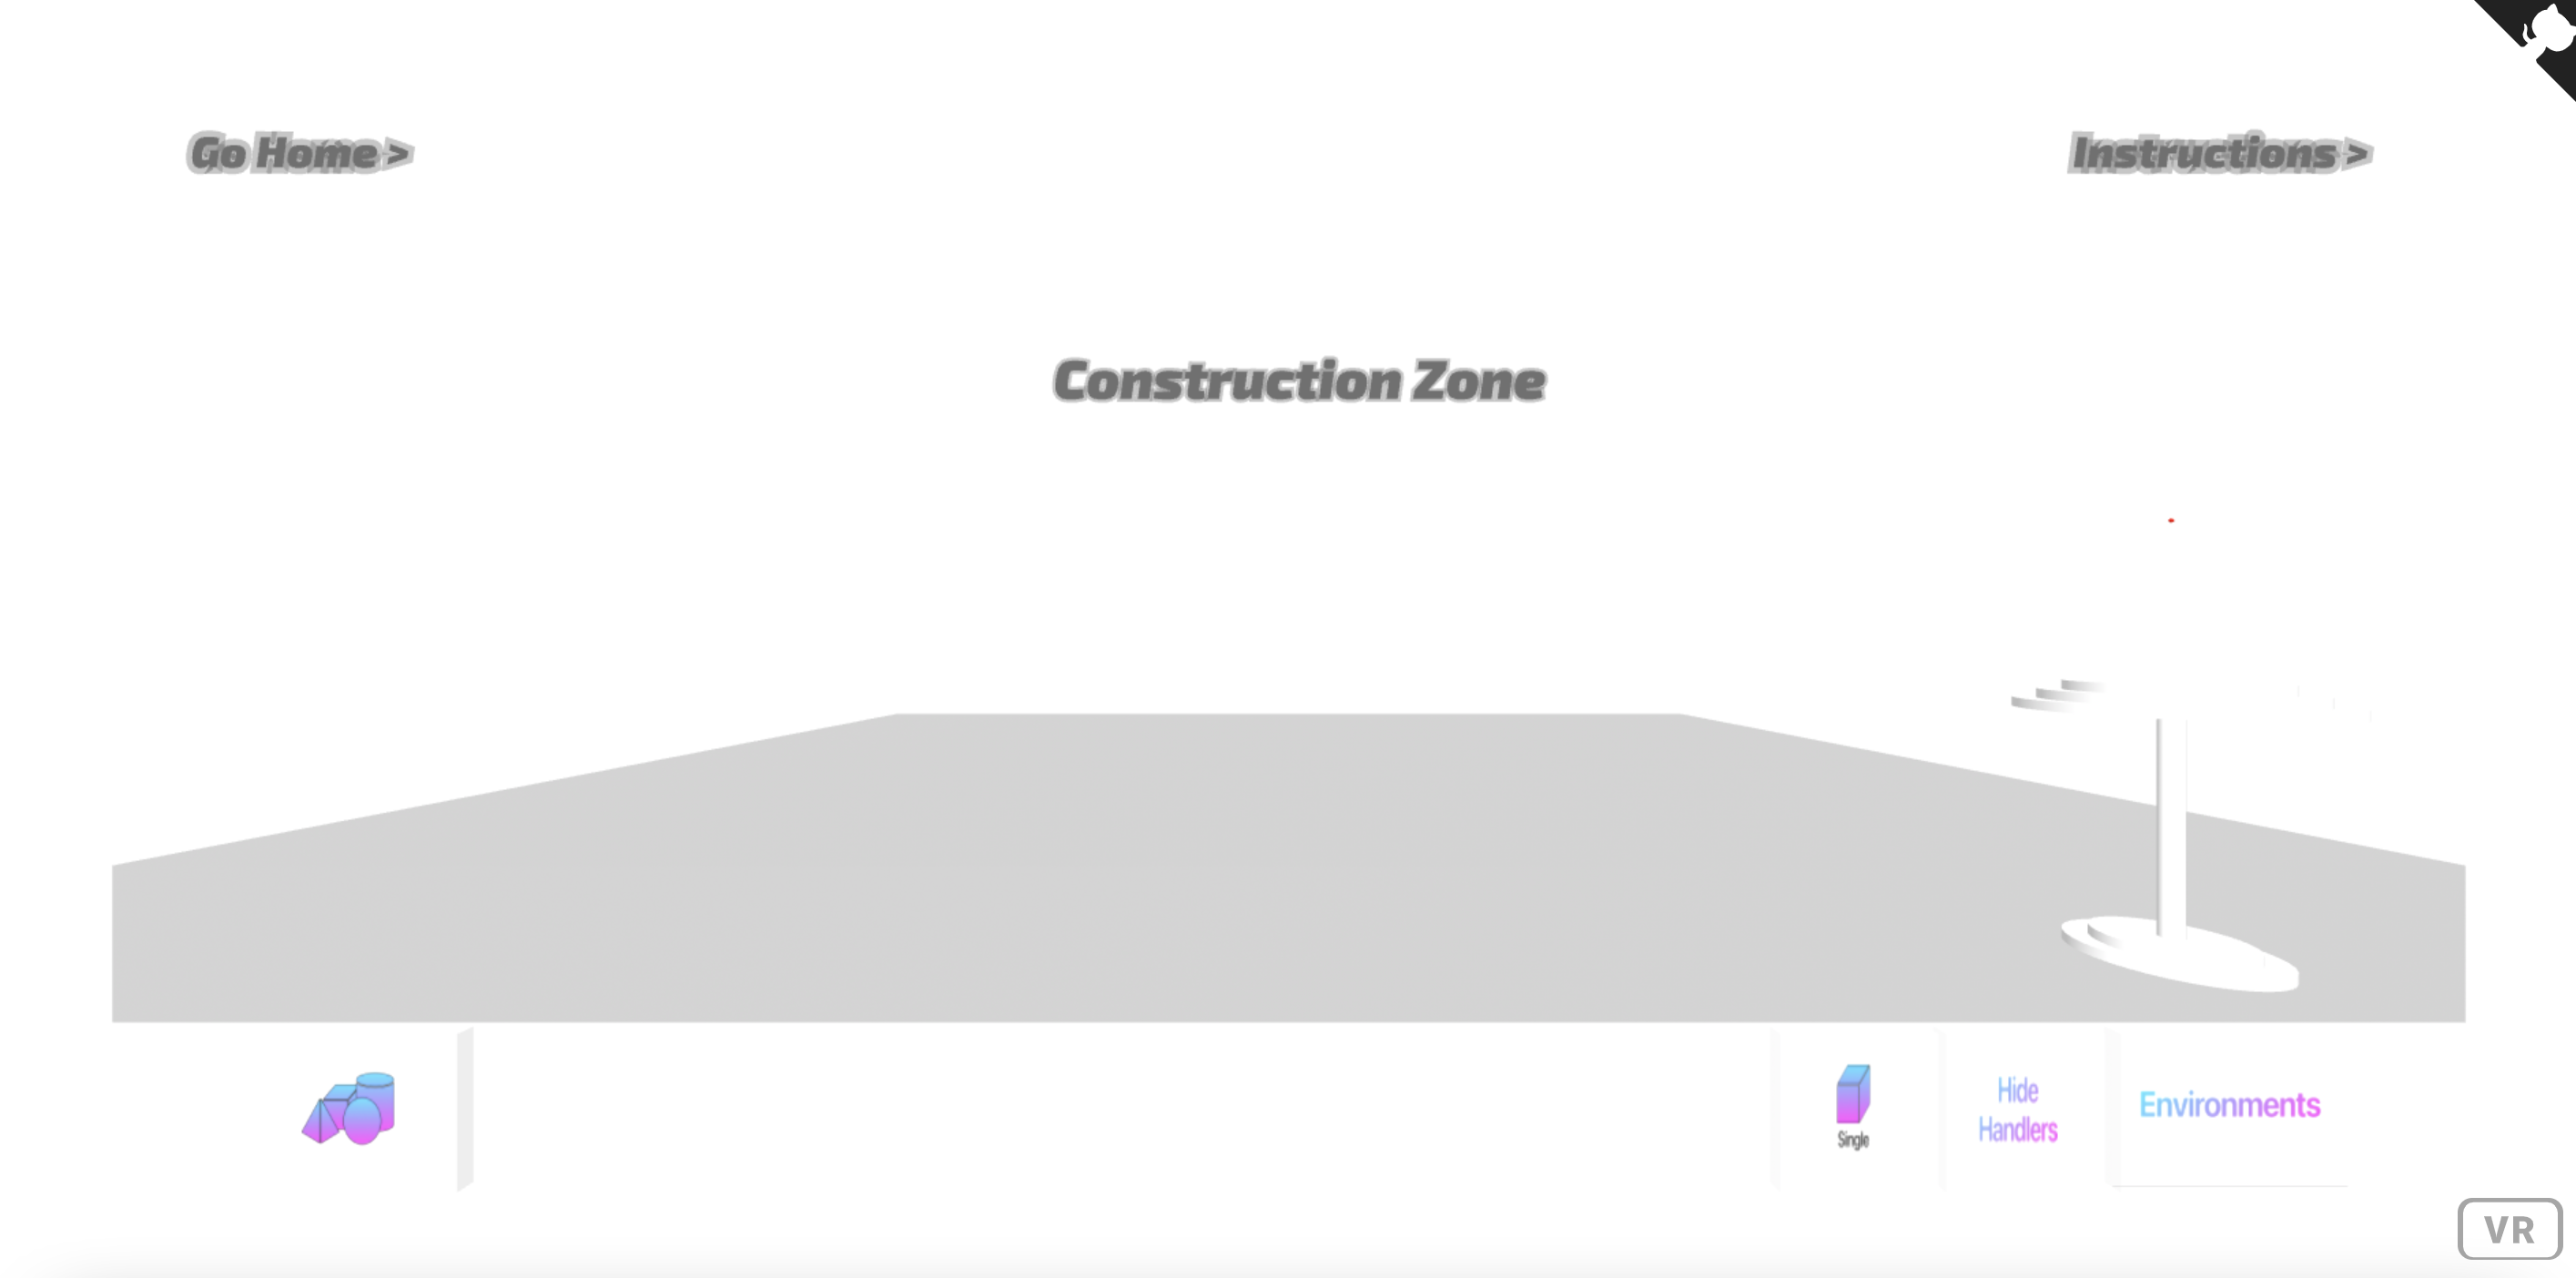
\includegraphics[width=10cm, keepaspectratio]{MemoriaTFG-JulianPerez/img/Captura de pantalla 2021-06-08 a las 19.06.47.png}
  \caption{Página Básica }\label{home}
\end{figure}

Por lo que observamos en el código, con dos elementos principales, como son el usuario y el podium, ya se tendría acceso a todas las funcionalidades de la aplicación.

Destacaré que mi aplicación no es un simple editor, si no que contiene diferentes componentes que pueden ser usados bien por separado, bien juntos en cualquier otra aplicación de este campo u otro.

\section{Implementación} 
\label{sec:Arquitectura resultante}
En esta sección más técnica explicaré la arquitectura de la aplicación y los componentes creados para la construcción de este proyecto y explicaré la función que ejercen cada uno de estos.

Comenzando con la arquitectura de la aplicación, partiré del esqueleto principal de esta.

\begin{verbatim}
<!DOCTYPE html>
<html>
 <head>
 </head>
<body>
<a-scene id="scn" overlay-visibility>
  <a-assets></a-assets>
  <!-- enviroment-->
  <a-entity id="env" environment="preset:forest"></a-entity>
  <!-- Podium -->
  <a-entity class="podium" podium></a-entity> 
  <!--User Camera-->
  <a-entity>
  <a-box id="showeditor" showeditor></a-box>
  <a-entity id="menu" menu></a-entity>
  <a-entity id="menuenv"></a-entity>
  <a-entity id="editor"></a-entity>
  <a-box id="showhandler" handlereditor></a-box>
  <a-box id="deletehandler" deletehandler></a-box>
  <a-box id="selectenviroments" selectenv></a-box>
  <a-entity gotohome ></a-entity>
  <a-entity gotoinstructiondesktop ></a-entity>
  </a-entity>
</a-scene>
 </body>
</html> 
\end{verbatim}

Como se puede ver en esta versión simplificada del código, este esta formado por diferentes elementos que contienen los distintos componentes creados.

Lo primero que nos encontramos es el elemento head, en el cual  se introduce todo lo necesario para que A-Frame y los distintos componentes, funcionen correctamente.

En el siguiente elemento, assets, se introducen todas las imagenes, modelos 3D y también un elemento llamado mixin que es un plantilla de creación de las figuras básicas para no repetir código en la creación de estas.

Tras el elemento assets, nos encontramos con el elemento que crea el ambiente de la escena y que será modificado dinámicamente mediante un componente que explicaré más adelante.

Tras este, nos encontramos con el elemento pódium en el cual generaré la figuras que vayamos creando.

Por último nos encontramos con el elemento usuario, el  padre de los elementos de menú de interacción de la escena.

Como ya he comentado, a cada uno de estos elementos se le añadirán los componentes, a continuación pasaré a explicarlos.

Clasificaré los componentes según el elemento al que afecte.

\begin{itemize}
    \item \textbf{Pódium}, Este componente se encarga de crear todas las figuras que componen el podium y su posición en la escena. Este es activado al generar el escenario y su función no es otra que tener una posición de referencia en la cual crear las figuras.
\end{itemize}

Los componentes que modifican el comportamiento del selector de figuras son:
\begin{itemize}
    \item \textbf{showeditor}, Es el encargado de generar las figuras disponibles para su creación y edición, a su vez genera el botón de acceso a los modelos 3D disponibles mediante la creación de otro componente. Este componente hace el uso de un evento encargado de escuchar si el elemento es pulsado, de este modo se activa el componente.
    
    \item \textbf{showmorefigure}, Componente generado a partir del anterior, encargado de crear cuatro botones con sus respectivos componentes, estos separan los modelos 3D en cuatro categorías distintas. Este componente reacciona al evento clicar, por lo que se activa al pulsar el botón.

    \item \textbf{show(vehicles/plants/animals/gadgets)}, Este componente acompaña a los cuatro botones generados mediante el componente anterior, si pulsamos cada uno de estos botones, te mostrará los diferentes modelos 3D. Por lo que este componente reacciona al mismo evento que los anteriores.

\end{itemize}

Los componentes que modifican los atributos de las figuras que vamos creando son:
\begin{itemize}
    \item \textbf{editentity}, La función de este componente es crear los elementos del menú modificación de la figura, cada uno con sus respectivos componentes, como se muestra en la figura 3.16. Este componente se activa al pulsar cualquiera de las 3 figuras básicas al abrir el menú de selector de figuras. 
    
    \item \textbf{changeattribute}, Este componente es creado por el anterior, y acompaña a las figuras de diferente color que se pueden ver en la parte del menú dedicada al cambio de color. El objetivo de este componente trata de extraer el atributo que contiene el color de las figuras del menú clicando en ellas y aplicárselo a la figura que he creado. 
    
    \item \textbf{(metalness/roughness/opacity)(up/down)}, Estos componentes se encuentran en los botones + y - de la parte del menú que te permite modificar los atributos de metalizado, rugosidad y opacidad de la figura, este es creado al pulsar una de las tres figuras principales. Accediendo a dichos atributos de la figura y modificándolos ya sea aumentándolos o disminuyéndolos, su objetivo es modificar dichos atributos.
    
    \item \textbf{size(up/down)(x/y/z)}, Estos componentes tienen el mismo comportamiento que los anteriores y son creados del mismo modo, pero su objetivo es modificar el atributo de escala de la figura, aumentándolo o disminuyéndolo pulsando los botones + o -.
    
    \item \textbf{rotation(up/down)(x/y/z)}, Igual al anterior con la diferencia que este se centra en el atributo de la rotación.
    
    \item \textbf{dotransparent}, La activación de este componente se genera al pulsar en el botón del menú dedicado para ello. El fin principal de este es modificar el atributo de transparencia  activándolo cuando se pulsa dicho botón.
    
    Los dos componentes siguientes no voy a desarrollarlos ya que tienen el mismo comportamiento que los anteriores pero dirigidos a los modelos 3D. No comparto componentes que realizan la mismo función pero sobre figuras básicas debido a que la escala de los modelos en 3D actúa de manera diferente que sobre las figuras básicas de A-Frame.
    \item \textbf{editorglts}
    \item \textbf{size(up/down)gltf(x/y/z)}
\end{itemize}

    
Sobre la funcionalidad modo grupo podemos distinguir los distintos componentes:
\begin{itemize}
    \item \textbf{handlereditor}, Este componente se genera al cargar el escenario y acompaña al botón que permite acceder a la funcionalidad del modo grupo. Este componente reacciona al evento clicar por lo que su activación y desactivación se realiza mediante la pulsación del botón. Cuando el componente esté activado y así lo mostrará la imagen del botón, creará un figura básica en el pódium que tomaré como manejador,a todas las figuras de la escena que sean clicadas en este momento se les añadirá un nuevo componente que permitirá unir dichas figuras.
    
    \item \textbf{posibilityofgroup}, Este componente se genera al pulsar una figura con el modo grupo activado, se encarga de crear una figura idéntica a la que hay en el escenario y en la misma posición, pero esta vez siendo hija del manejador, de esta manera, cuando el manejador sea desplazado estas se moverán del mismo modo.
    
    \item \textbf{deletehandler}, Componente generado al cargar el escenario acompañando en el botón que nos permite ocultar y mostrar los manejadores. Este componente se activa pulsando dicho botón y su objetivo es modificar el atributo encargado de la opacidad modificándolo para así poder mostrar los manejadores cuando este esté desactivado u ocultándolos cuando se encuentre activo.
\end{itemize}

Los componentes que se relacionan con el menú de ambientes son:
\begin{itemize}
    \item \textbf{selectenv}, Este componente es generado al cargar el escenario y acompaña al botón que permite acceder a los diferentes ambientes que añadir a la escena. Al pulsar el botón que contiene el componente crea distintos botones con previsualizaciones de la escena con los respectivos ambientes y con sus respectivos componentes.
    \item \textbf{env(1/2/3/4/5)}, Componente generados por el anterior cuya función es modificar el ambiente de la escena y añadir el ambiente elegido por el usuario según el botón pulsado.
    
\end{itemize}

Por último, los componentes que añaden comportamiento a los botones para ir a la pantalla de incio y a la de instrucciones son:

\begin{itemize}
    \item \textbf{gotoeditor(glasses)} Este componente se localiza en la parte superior de la escena y es creado al generar la escena. Su función es la de llevar al usuario a la escena de creación del editor. La activación de este componente se realiza pulsando el propio texto. Este componente solo es generado en la página principal y en la de instrucciones.
    
    \item \textbf{gotohome(glasses)}, mismo comportamiento que el anterior, pero en este caso solo se generará en la pagina de creación y en la de instrucciones.
    
    \item \textbf{otoinstructions(glasses)}, mismo comportamiento que los anteriores, pero generado en la página principal y en la página de creación.
\end{itemize}

Para finalizar, cabe desatacar los componentes que nos ofrece A-frame y hacemos uso en nuestra aplicación:
\begin{itemize}
    \item \textbf{clickable}, Este componente nos aporta, al elemento que lo contiene, la cualidad de poder ser clicado para futuros eventos, este componente es utilizando en casi todos nuestros elementos de la aplicación.
    \item \textbf{grabbable}, Este componente nos permite arrastrar a cualquier parte de la escena los elementos que lo contengan. 
\end{itemize}


%%%%%%%%%%%%%%%%%%%%%%%%%%%%%%%%%%%%%%%%%%%%%%%%%%%%%%%%%%%%%%%%%%%%%%%%%%%%%%%%
%%%%%%%%%%%%%%%%%%%%%%%%%%%%%%%%%%%%%%%%%%%%%%%%%%%%%%%%%%%%%%%%%%%%%%%%%%%%%%%%
% CONCLUSIONES %
%%%%%%%%%%%%%%%%%%%%%%%%%%%%%%%%%%%%%%%%%%%%%%%%%%%%%%%%%%%%%%%%%%%%%%%%%%%%%%%%
\cleardoublepage
\chapter{Conclusiones}
\label{chap:conclusiones}
En este punto de la memoria, echaré la vista atrás y visualizaré si se lograron los objetivos presentados en el capítulo~\ref{sec:intro}, también comentaremos los problemas surgidos durante la realización del mismo.

De manera general, se puede decir que he conseguido todos los objetivos propuestos al inicio del proyecto.

Respecto de los objetivos generales realizados, 

\begin{itemize}
    \item La creación de un editor de escena en realidad virtual.
    \item Este editor está basado en las tecnologías tanto de A-Frame como de WebGL
    \item El funcionamiento tanto en un entorno de escritorio mediante el navegador web como en modo realidad virtual mediante las Oculus Quest.
\end{itemize}

Sobre los objetivos específicos conseguidos nos encontramos. 
\begin{itemize}
    \item La creación tanto de la página principal y página de usuario.
    \item En cuanto a las funcionalidades propuestas
    \begin{itemize}
        \item La creación de un menú desde el cual crear y modificar distintos atributos de las figuras.
        \item La creación del modo grupo, gracias a él podremos construir una figura mediante la unión de varias.
        \item La posibilidad de ocultamiento de los manejadores del escenario.
        \item La oportunidad de modificar el ambiente del escenario.
    \end{itemize}
    \item Añadidura de movimiento al usuario en ambas versiones.
    \item El uso de la plataforma GitHub para el alojo del proyecto, tanto de la aplicación como de la memoria como la Web. Esto se puede ver reflejado en los links adjuntos en el capitulo tres de esta memoria.
\end{itemize}

\section{Aplicación de lo aprendido}
\label{sec:aplicacion}

Durante la realización del grado, he obtenido conocimiento sobre distintos temas, una de ellas la programación, en distintas asignaturas, la cual me ha permitido desarrollar este proyecto, tanto a la hora de aplicar lo aprendido como la manera de aprender lo necesario para el desarrollo de este.

Algunas asignaturas de las que hablo son:
\begin{enumerate}  
\item Servicio y Aplicaciones Telemáticas, Esta asignatura me ayudo con el uso del navegador, tanto de la consola, como el tratamiento de errores, el conocimiento de la estructura del DOM en el cual poder añadir elementos y eventos y en menor medida el lenguaje HTML.
  \item Desarrollo de Aplicaciones Telemáticas, en la cual aprendí el lenguaje HTML y en menos medida el lenguaje JavaScript.
  \item Ingeniería en Sistemas de la Información, esta asignatura fue muy importante para el manejo de la plataforma GitHub y el tratamiento de control de versiones.
\end{enumerate}
En resumen, todas las asignaturas relacionadas con la programación me han aportado distintos conocimientos, ya sea los distintos lenguajes de programación o aprender a resolver los distintos problemas que han ido surgiendo a lo largo de la creación del proyecto.

\section{Lecciones aprendidas}
\label{sec:lecciones_aprendidas}

Gracias a la creación de este trabajo de fin de grado he adquirido diversos conocimientos y he aprendido muchas lecciones que pasaré a desarrollar a continuación.
\begin{enumerate}
  \item Uno de los principales y más usados en este proyecto, A-Frame. Dentro de este framework incluimos:
  \begin{itemize}
      \item Creación de escenas
      \item Creación de componentes, los cuales reaccionan con los elementos de la escena.
      \item Construcción de distintos elementos de este framework como puede ser, la cámara, la iluminación, el ambiente, las figuras etc.
  \end{itemize}
  \item El lenguaje JavaScript, ya que este no se enseña en profundidad en la carrera y este trabajo me ha permitido aumentar el conocimientos sobre este. la creación de eventos y la modificación en tiempo real de los elementos de la escena es un de las funciones de este lenguaje que se incluyen en el proyecto.
  \item El uso de los entornos de realidad virtual ya sea tanto en el navegador como con las gafas de realidad virtual.
  \item El aumento del conocimiento de las herramientas de desarrollo de este proyecto, en las que se incluyen:
  \begin{itemize}
      \item LaTeX para la creación de textos técnicos como este.
      \item PyCharm para el desarrollo del código de la aplicación
      \item GitHub, como ya he contado anteriormente para el alojo del código y el tratamiento de control de versiones.
  \end{itemize}
\end{enumerate}


\section{Trabajos futuros y esfuerzo dedicado}
\label{sec:trabajos_futuros}

Como se suele decir en un proyecto de este tipo, ningún proyecto se termina, siempre se pueden añadir nuevas funcionalidades que amplíen y mejoren este, por lo que a continuación enumeraré una seria de ideas para poder incluir en un futuro.

\begin{itemize}
    \item La posibilidad de poder guardar el escenario creado, ya sea una figura o todo el escario, de este modo poder añadir versatilidad al proyecto y podernos llevar las figuras creadas a otros tipos de escenarios.
    \item La posibilidad de poder modificar los atributos de las figuras, directamente en estas, y no mediante un menú. En el caso del navegador, con el uso del ratón y en el caso de la realidad virtual, directamente con los mando o con las manos.
    \item Poder modificar las figuras de una manera más especifica, por ejemplo poder eliminar una parte de la figura.
    \item Añadir más posibles ambientes al escenario.
    \item Añadir más modelos 3D al escenario.
    \item Añadir más físicas a las figuras del escenario, como pueden ser, gravedad.
\end{itemize}

Sobre el tiempo dedicado a este proyecto han sido unos 10 meses. He ido realizando el trabajo mientras realizaba mis prácticas en empresa. Un gran porcentaje de este, fue realizado los fines de semana y entre semana tras salir del trabajo.
%%%%%%%%%%%%%%%%%%%%%%%%%%%%%%%%%%%%%%%%%%%%%%%%%%%%%%%%%%%%%%%%%%%%%%%%%%%%%%%%
%%%%%%%%%%%%%%%%%%%%%%%%%%%%%%%%%%%%%%%%%%%%%%%%%%%%%%%%%%%%%%%%%%%%%%%%%%%%%%%%
% BIBLIOGRAFIA %
%%%%%%%%%%%%%%%%%%%%%%%%%%%%%%%%%%%%%%%%%%%%%%%%%%%%%%%%%%%%%%%%%%%%%%%%%%%%%%%%

\cleardoublepage

% Las siguientes dos instrucciones es todo lo que necesitas
% para incluir las citas en la memoria
\bibliographystyle{abbrv}
\bibliography{memoria}  % memoria.bib es el nombre del fichero que contiene
% las referencias bibliográficas. Abre ese fichero y mira el formato que tiene,
% que se conoce como BibTeX. Hay muchos sitios que exportan referencias en
% formato BibTeX. Prueba a buscar en http://scholar.google.com por referencias
% y verás que lo puedes hacer de manera sencilla.
% Más información: 
% http://texblog.org/2014/04/22/using-google-scholar-to-download-bibtex-citations/

\end{document}
